\documentclass[reprint,amsmath,amssymb,aps,pre,showkeys,showpacs,nofootinbib]{revtex4-1}
% Latex
\usepackage[english]{babel}
\usepackage[utf8]{inputenc}
\usepackage[T1]{fontenc}
% Xelatex
%\usepackage{polyglossia}
%\usepackage{fontspec}
%\setdefaultlanguage{english}
%\setmainfont{DejaVu Sans}
%\setsansfont{DejaVu Sans}
%\setmonofont{DejaVu Sans Mono}
\usepackage{bm}
\usepackage{cleveref}
\usepackage{xcolor}
\usepackage{algpseudocode}
\usepackage{graphicx}
\usepackage{subfigure}

\newtheorem{definition}{Definition}

\definecolor{light-gray}{gray}{0.95}
\newcommand{\code}[1]{\colorbox{light-gray}{\texttt{#1}}}
% When cleveref fails to do its job
\newcommand{\apref}[1]{Appendix \ref{#1}}

\begin{document}
\preprint{APS/123-QED}

\author{Aleksei Samarin\textsuperscript{1,2}}
\author{Vasily Postnicov\textsuperscript{1}}
\author{Marina Karsanina\textsuperscript{1}}
\author{Efim Lavrukhin\textsuperscript{1,2}}
\author{Dina Gafurova\textsuperscript{3}}
\author{Aleksey Khlyupin\textsuperscript{1}}
\author{Kirill Gerke\textsuperscript{1}}
\email{kg@ifz.ru}

\affiliation{\textsuperscript{1}Schmidt Institute of Physics of the Earth of
  Russian Academy of Sciences, Moscow, 107031, Russia}
\affiliation{\textsuperscript{2}Computational Mathematics and Cybernetics,
  Lomonosov Moscow State University, Moscow, 119991, Russia}
\affiliation{\textsuperscript{3}Oil and Gas Research Institute Russian Academy
  of Sciences (OGRI RAS) 3, Gubkina st., Moscow, 119333, Russian Federation}

\title{Evaluation of classical correlation functions from 2/3D images on CPU and
  GPU architectures: introducing CorrelationFunctions.jl}

\begin{abstract}
  What have we done?
\end{abstract}

\maketitle

\section{Background and motivation}
\label{sec:background}
Materials are ubiquitous both in nature and in industrial human activities, and
their physical properties are interconnected to
structure\cite{Torquato_book}\cite{Sahimi_book}\cite{Adler_recon}. The information
about the structure usually comes in the way of 2D and 3D images obtained by
microscopy, tomography and other related methodologies. This structural
information can be used for numerous types of analysis, including simulations of
different processes within studied materials or evaluation of their properties
using so-called pore-scale modelling. Unlike computational modelling techniques
a whole class of approximate methods exists including (rigorous) bounds that
allows very fast estimations of physical properties albeit the bounds themselves
are too wide to be applicable in majority of practical problems. Nonetheless, it
is noteworthy that such bounds are originally based on structural descriptors in
the form of correlation functions.

Two ways exist to obtain correlation functions for a given structure at hand:
measure them either experimentally with the help of scattering intensity or
from digital images. None is perfect, as the first approach suffers from the
limitation of CFs that can be obtained this way, while the second one provides
information with limited resolution or/and resolution to field-of-view ratio. In
addition to the resolution conundrum, the most useful imaging methods such as
X-ray computed tomography (XCT) and scanning electron microscopy (SEM) provide
gray-scale images (e.g., X-ray attenuation or electron back-scattering
distributions) due to their underlying physical principles and require labeling
of constituent phases (this is called segmentation) before computation of
CFs. If properly segmented, high-resolution digital images do provide a
possibility to compute any correlation function and, thus, possibility to
address numerous fundamental and practical research problems.

Correlation functions (CFs) as invaluable universal descriptors of structure are
utilized in a multitude of scientific disciplines: material sciences, rock
physics, soil physics and hydrology, cosmology and food engineering, biology and
many others. Computed from 2D and 3D images, CFs can be applied to:
\begin{enumerate}
  \item to characterize the morphology and representativeness via correlation
    lengths;
  \item to perform stochastic reconstructions from experimentally measured CFs
    or 2D to 3D reconstructions based on CFs that can be extracted from less
    dimensions or through penetrable sphere model;
  \item compare different structures to each other, including verification of
    stochastic reconstructions;
  \item compress structural information in the form of raw or parameterized CFs
    with the possibility to recover the structure using stochastic
    reconstruction
  \item describe structural dynamics under different boundary conditions;
  \item extract structural features for deep learning;
  \item fuse multi-scale images and structural information as obtained by
    different methods into a single digital model;
  \item quantify spatial heterogeneity.
\end{enumerate}

Stochastic reconstruction is a separate huge topic, as this approach allows to
solve an inverse problem and recover structure from known set of correlation
functions. This ability for recovery serves as the basis for majority of usages
in the list above. While it is necessary to compute CFs from digital images as a
target set for stochastic reconstructions, they rely more on efficient
recomputations or optimizations, e.g., re-evaluation during simulated
annealing. Such optimizations are not the part of the computational package and
are not considered in this work.

There are different types of correlation functions that in general describe some
probabilities. The main parameter of any correlation function is the number of
points that are utilized to evaluate such a probability. While so-called
$n$-point probability function\cite{Torquato_book} will totally describe any
structure in the limit of $n \rightarrow$ number of voxels/pixels on the image,
computing or storing such a function is not practical. Based on information
content, it was shown that increasing the number of point $n > 2$ only
marginally improves the quality of the structure quantification and these
improvements decay with increasing $n$. For stochastic reconstruction purposes
computation of higher-order statistics will, arguably, not be balanced by
increased number of points, but this is the topic of active research. For
aforementioned reasons, we mainly focus on 2-point statistics, leaving the
possibility to include higher order CFs in the future work. The simplest 2-point
probability function ($S_2$ or autocorrelation) actually arise from small angle
scattering experiments and measures the probability that both ends of line
segment with a given length fall into the same phase. Other types include the
probability of a whole line segment to fall into the phase ($L_2$ function) or
to lie on the interface between phases ($F_{ss}$ function), and mainly originate
from aforementioned bounds on physical properties such as permeability and
elasticity. The general idea of computation of different 2-point CFs is shown in
\cref{fig:functions}. All major details and numerous analytical cases can be
found in seminal work of Torquato \cite{Torquato_book}. To all CFs described in this
book and applicable to digital images we shall refer as to classical correlation
functions.

\begin{figure}[ht]
  \centering
  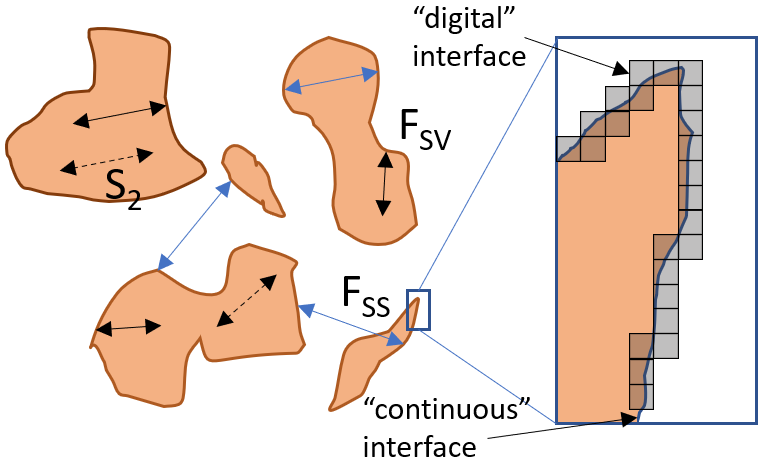
\includegraphics[width=0.9\linewidth]{images/corr.png}
  \caption[]{A schematic depiction of a binary porous media (pores are shown in
    color) with examples of positive events for surface $F_{ss}$, $F_{sv}$ and
    two-point probability $S_2$ correlation functions. The zoomed in area
    represents the difference between the true ``continuous'' interface in
    between pore and solid phases with pixelized ``digital'' interface emerging
    due to limited resolution of digital images.}
  \label{fig:functions}
\end{figure}

While evaluation of correlation functions from 2D and 3D images was a topic of
numerous research papers, the information is highly fragmented, especially in
terms of algorithms and their implementation in the code. Some snippets of code
are available for some functions, but they lack general API and are usually
implemented in proprietary interpreted languages such as Matlab. Due to a recent
leap forward in GPU-based computations, some papers describe computations on
this architecture, but the code is usually not provided. All in all, the
efficient and open-source single API solution utilizing both CPU and GPU
architectures is currently absent.

The aim of this paper is to establish a general open-source solution allowing to
compute all classical correlation functions. This solution should be well
documented with all computational algorithms explained, it should also leverage
on recent advances in programming high-intensity computations and utilize both
CPU and GPU power. Our answer in the form of \code{CorrelationFunctions.jl}
package allows to compute numerous CFs easily on any operating system. The
manuscript describing the package is organized as follows: in \cref{sec:math} we
introduce a reader to the most common and useful correlation functions,
\cref{sec:map} presents all algorithmic details for computing full CFs maps (map
method, full 2-point statistics for a given image). In \cref{sec:scan} we
provide all algorithmic details for CFs computation in directions (scanning
method). In \cref{sec:verification} we verify the all computations based on
known analytical solutions. \cref{sec:efficiency} deals with computational
efficiency of our code, we compare computational times for 2D and 3D images of
different sizes for scanning and map methods as evaluated using either CPU or
GPU. In \cref{sec:examples} some application examples are provided, including
CFs evaluation for multi-phase materials. Finally, \cref{sec:summary} summarizes
all results and outlines possible future improvements.

\section{Introduction to the correlation functions}
\label{sec:math}
In practice porous media are often described with special descriptors called
``correlation functions''. In this section we provide a brief introduction to
these functions which can also be found in \cite{Torquato_book}. The functions
supported by our package are:
\begin{itemize}
\item Lineal-path function $L_2$.
\item Two-point function $S_2$.
\item Cluster function $C_2$.
\item Surface-surface function $F_{ss}$.
\item Surface-void function $F_{sv}$.
\item Pore size function $P$.
\item Chord length function $p$.
\item Phase cross-correlation function $\rho_{ij}$
\end{itemize}

One of basic correlation functions is a lineal path function which is defined as
follows for homogenous media:
\begin{definition}
  Lineal path function $L_2^{(i)}(\mathbf{r})$ equals to probability that a
  vector $\mathbf{r}$ lies wholly in phase $i$ when randomly thrown into the
  sample.
\end{definition}
If a sample is isotropic a vector $\mathbf{r}$ can be replaced with its length
$r$ and the definition becomes:
\begin{definition}
  Lineal path function (for isotropic media) $L_2^{(i)}(r)$ equals to
  probability that a line segment of length $r$ lies wholly in phase $i$ when
  randomly thrown into the sample.
\end{definition}

Another function of big importance is a two-point correlation function $S_2$. A
definition for homogenous media is as follows:
\begin{definition}
  Two point function $S_2^{(i)}(\mathbf{r})$ equals to probability that both ends
  of a vector $\mathbf{r}$ lie in phase $i$ when the vector is randomly thrown
  into the sample.
\end{definition}
For isotopic media a vector $\mathbf{r}$ can be again reduced to a scalar value
$r$ (i.e. a correlation function depends only on length of a vector and not on
its direction.) Mathematically this definition can be expressed with the
following equation:
\begin{equation}
  S_2^{(i)}(\mathbf{r}) = \langle I^{(i)}(\mathbf{x}) I^{(i)}(\mathbf{x} +
  \mathbf{r}) \rangle
  \label{eq:s2-def}
\end{equation}
where $I^{(i)}$ is an indicator function for a set of all points belonging to
the phase $i$ and $\langle \cdots \rangle$ is an average over all xs.

A function closely related to $S_2$ is phase cross-correlation function
$\rho_{ij}$ which is defined with the following equation:
\begin{equation}
  \rho_{ij}(\mathbf{r}) = \langle I^{(i)}(\mathbf{x}) I^{(j)}(\mathbf{x} +
  \mathbf{r}) \rangle
  \label{eq:cross-def}
\end{equation}

The next function is a cluster function $C_2$.
\begin{definition}
  Cluster function $C_2^{(i)}(\mathbf{r})$ equals to probability that both
  ends of a vector $\mathbf{r}$ lie in the same cluster when the vector is
  randomly thrown into the sample. A cluster is a set of points of the same
  phase $i$ where any to points can be connected by a path lying entirely in
  that phase.
\end{definition}

The next two functions describe surface of a sample. These functions are
surface-surface and surface-void functions. For homogenous media their
definitions are:
\begin{definition}
  Surface-surface function $F_{ss}^{(i)}(\mathbf{r})$ equals to probability that
  both ends of a vector $\mathbf{r}$ touch the interface of phase $i$ when the
  vector is randomly thrown into the sample.
\end{definition}
and
\begin{definition}
  Surface-void function $F_{sv}^{(i)}(\mathbf{r})$ equals to probability that
  one end of a vector $\mathbf{r}$ touches the interface of phase $i$ and the
  other end touches the void phase when the vector is randomly thrown into the
  sample.
\end{definition}
If we introduce an interface indicator function
\begin{equation*}
  M^{(i)}(\mathbf{r}) = | \nabla I^{(i)}(\mathbf{r}) |
\end{equation*}
we can define these functions mathematically as
\begin{align}
  F_{ss}^{(i)}(\mathbf{r}) &= \langle M^{(i)}(\mathbf{x}) M^{(i)}(\mathbf{x} +
  \mathbf{r}) \rangle \label{eq:fss-def} \\ 
  F_{sv}^{(i)}(\mathbf{r}) &= \langle M^{(i)}(\mathbf{x}) I^{(void)}(\mathbf{x}
  + \mathbf{r}) \rangle \label{eq:fsv-def}
\end{align}
As always, there are versions of these functions applicable to scalar argument
for isotropic media.

Pore size function $P(\delta)$ is a probability density function defined as
follows:
\begin{definition}
  $P(\delta)d\delta$ = Probability that a randomly chosen point in a set of points
  belonging to the void phase lies at a distance between $\delta$ and $\delta + d\delta$
  from the nearest point on the pore-solid interface.
\end{definition}

Finally, a chord length function $p^{(i)}(r)$ is defined as follows:
\begin{definition}
$p^{(i)}(r)dz$ = Probability of finding a chord of length between $r$ and $r+dr$
in phase $i$. Chords are all of the line segments between intersections of an
infinitely long line with the two-phase interface.
\end{definition}

\verb+CorrelationFunctions.jl+ is capable to compute all these
functions. Usually there are two implementations for a function. The first
implementation computes a correlation function in specific predefined directions
(i.e. orientation of test vectors thrown into a sample is fixed). There are one
predefined direction in 1D case, four directions in 2D case and thirteen
directions in 3D case. This implementation is somewhat slow but requires much
less memory than the second one. The second implementation computes a
correlation function in all directions and is faster but requires much memory.
These implementations are contained in \code{Directional} and \code{Map} modules
of the package correspondingly.

These functions can work in periodic and non-periodic modes. Periodic mode
assumes that an input sample is periodically continued to the whole Euclidean
space. Non-periodic mode assumes zero-padded input.

\section{The map approach.}
\label{sec:map}
Definition \cref{eq:s2-def} can be rewritten as follows:
\begin{equation}
  S_2^{(i)}(r) = \frac{F^{-1} [|F [A^{(i)}](z)|] (r)}{N(r)} \label{eq:s2-ft}
\end{equation}
where $A^{(i)} \xleftarrow{I^{(i)}} A$ is a binary array obtained by element-wise
application of interface indicator $I^{(i)}$ to an input $A$, $F$ is a discrete
Fourier transform operator and $N(r)$ is a total number of trials (vectors
thrown into sample).












In this approach we actively use fast Fourier transform (FFT)
to compute some correlation function ($S_2, F_{ss}, F_{sv}, C_2$)
in all directions.
The FFT algorithm let us compute auto and cross-correlation fast,
especially on GPU.

Lineal-path function doesn't have FFT realization,
therefore, we use different approach.

\subsection{Lineal-path function}

Since the method for calculating $l_2$ using the FFT is unknown,
we use the direct approach:
scan the image in each selected direction.
\textcolor{red}{[czech paper]} uses this method,
but our approach saves porosity when rotating the image.
The top-level algorithm is described below, 
and the details are placed in the appendix.

\begin{algorithmic}[1]
  \Procedure{l2\_map}{$a, periodic, directions$}
    \ForAll{$direction \in directions$}
      \State $rotated \gets rotate(a, direction, periodic)$
      \State $l2[direction] \gets scan\_l2(aligned, periodic)$
    \EndFor
    \State \textbf{return} $l2$
  \EndProcedure
\end{algorithmic}

Align and rotate --- simple operations with linear computational complexity.
Therefore, the complexity of the entire algorithm depends linearly 
on the number of directions and on the size of the image.

\subsection{Correlation map}

\subsubsection{Auto- and cross-correlation using FFT}

All subsequent functions are auto- or cross-correlations.
Therefore, here we describe a method to compute them using FFT.

\begin{algorithmic}[1]
  \Procedure{cross\_correlation}{$a, b$}
    \State $A \gets rfft(a)$\Comment{Real fast Fourie transform}
    \State $B \gets rfft(b)$
    \ForAll{$i \in CartesianIndices(A)$}
      \State $C[i] \gets conj(A[i]) \cdot B[i]$
    \EndFor
    \State $c = irfft(C)$ 
    \Comment{inverse rfft}
    \State \textbf{return} $c$
  \EndProcedure
\end{algorithmic}

One can use cross-correlation to compute auto-correlation,
but special function would permorm better.

\begin{algorithmic}[1]
  \Procedure{auto\_correlation}{$a$}
    \State $A \gets rfft(a)$
    \ForAll{$i \in CartesianIndices(A)$}
      \State $C[i] \gets |A[i]|^2$
    \EndFor
    \State $c = irfft(C)$ 
    \State \textbf{return} $c$
  \EndProcedure
\end{algorithmic}

CartesianIndices --- all indices of multidimensional array,
therefore, the for loop describe elementwise operations
and have linear computational complexity $O(n)$.
For both functions computational complexity is $O(n\ log(n))$.

It is worth noting, that the FFT approach imply
periodic boundary conditions by design.

\subsubsection{Total number of trials}

$auto\_correlation$ and $cross\_correlation$ return non-negative number
of success trials \cref{eq:probability}.
To compute probability we need to count total number of trials.
This value depends on boundary conditions.
We realize two types: periodic and non-periodic (flat).

\begin{algorithmic}[1]
  \Procedure{total}{$a, periodic$}
    \State $m, n \gets size(a)$
    \If{periodic}
      \ForAll{$i \in range(0, m - 1)$}
        \ForAll{$j \in range(0, n - 1)$}
          \State $total[i, j] \gets m \cdot n$
        \EndFor
      \EndFor
    \Else
      \ForAll{$i \in range(-m + 1, m - 1)$}
        \ForAll{$j \in range(-n + 1, n - 1)$}
          \State $i' \gets mod(i, 2m - 1)$
          \State $j' \gets mod(j, 2n - 1)$
          \State $total[i', j'] \gets |m - i| \cdot |n - j|$
        \EndFor
      \EndFor
    \EndIf
    \State \textbf{return} $total$
  \EndProcedure
\end{algorithmic}

Described function is for 2D images,
for 1D and 3D images realization is similar.

if n is the number of pixels, then computational complexity
of this funciton is $O(n)$.

\subsubsection{Two-point funciton}

We realize two boundary conditions: periodic and non-periodic (flat).
For non-periodic boundary conditions one need to double image size
by padding new values with zeros.
Thus, if original image is $(m \times n)$,
then expanded image will have size $(2m - 1 \times 2n - 1)$.

\begin{algorithmic}[1]
  \Procedure{s2\_map}{$a, phase, periodic$}
    \State $a_1 \gets a = phase$
    \If{periodic}
      \State $a_2 \gets a_1$
    \Else
      \State $a_2 \gets expand(a_1)$\Comment{double image size by padding new values with zeros}
    \EndIf
    
    \State $success \gets AUTO\_CORRELATION(a_2)$

    \State $total \gets TOTAL(a, periodic)$

    \ForAll{$i \in CartesianIndices(success)$}
      \State $s2[i] \gets success[i]\ /\ total[i]$
    \EndFor
    
    \State \textbf{return} $s2$
  \EndProcedure
\end{algorithmic} 

if n is the number of pixels, then computational complexity
of this funciton is $O(n\ log(n))$.

\subsubsection{Phase cross-correlation funciton}

\begin{algorithmic}[1]
  \Procedure{cc\_map}{$a, b, periodic$}
    \If{periodic}
      \State $a_1 \gets a$
      \State $b_1 \gets b$
    \Else
      \State $a_1 \gets expand(a)$
      \State $b_1 \gets expand(b)$
    \EndIf
    
    \State $success \gets CROSS\_CORRELATION(a_1, b_1)$

    \State $total \gets TOTAL(a, periodic)$

    \ForAll{$i \in CartesianIndices(success)$}
      \State $cc[i] \gets success[i]\ /\ total[i]$
    \EndFor

    \State \textbf{return} $cc$
  \EndProcedure
\end{algorithmic}

if n is the number of pixels, then computational complexity
of this funciton is $O(n\ log(n))$.

\subsection{Surface-surface function}

Computation of surface-surface function consists of two steps 
\textcolor{red}{[link to surface paper]}:
\begin{enumerate}
  \item extracting surface $M = \nabla I(a)$
  \item computing $F_{ss} = S_2(M)$
\end{enumerate}

For surface extraction we use `imgradient' function
and Sobel kernel as default kernel, 
both defined in ImageFiltering.jl package \textcolor{red}{[add link]}.

\begin{algorithmic}[1]
  \Procedure{surf\_surf}{$a, phase, periodic, kernel$}
    \State $a_1 \gets a = phase$
    \State $M \gets imgradient(a_1, kernel)$
    \State $Fss = S2\_MAP(M, periodic)$
    \State \textbf{return} $Fss$
  \EndProcedure
\end{algorithmic}

if n is the number of pixels, then computational complexity
of this funciton is $O(n\ log(n))$.

\subsection{Surface-void function}
Computation of surface-void function consists of three steps 
\textcolor{red}{[link to surface paper]}:
\begin{enumerate}
  \item extracting surface $M = \nabla I(a)$
  \item extracting void phase $V = I_v(a)$
  \item computing $F_{sv} = cross\_correlation(M, V)$
\end{enumerate}

\begin{algorithmic}[1]
  \Procedure{surf\_void}{$a, phase, periodic, kernel$}
    \State $a_1 \gets a = phase$
    \State $M \gets imgradient(a_1, kernel)$
    \State $V \gets a = 0$
    \State $Fsv = CC\_MAP(M, V, periodic)$
    \State \textbf{return} $Fsv$
  \EndProcedure
\end{algorithmic}

if n is the number of pixels, then computational complexity
of this funciton is $O(n\ log(n))$.

\subsection{Cluster funciton}

Computation of cluster function consists of three steps
\begin{enumerate}
  \item label different clusters with distinct integers
  \item compute $S_2$ map for every cluster
  \item add up all maps
\end{enumerate}

For labeling we use `label\_components' function from
Images.jl package \textcolor{red}{[add link]}.

\begin{algorithmic}[1]
  \Procedure{cluster\_map}{$a, phase, periodic$}
    \State $a_1 \gets a = phase$
    \State $labeled\_a \gets label\_components(a_1, periodic)$
    \State $number\_of\_labels = maximum(labeled\_a)$
    \ForAll{$label \in range(1, number\_of\_labels)$}
      \State $b \gets labeled\_a = label$
      \If{label = 1}
        \State $c2 \gets S2\_MAP(b, periodic)$
      \Else
        \State $c2 \gets c2 + S2\_MAP(b, periodic)$
      \EndIf
    \EndFor
    \State \textbf{return} $c2$
  \EndProcedure
\end{algorithmic}

if n is the number of pixels and N is the number of clusters, then computational complexity
of this funciton is $O(N\ n\ log(n))$.

\section{The scan approach.}
\label{sec:scan}
In this approach, the input array is cut in parallel slices (``scanned'') along
each requested direction. Each slice is then analyzed independently as
one-dimensional system and the result is accumulated into \code{CorrelationData}
structure. In the following sections we provide the algorithms for computation
of the functions given in \cref{sec:math}.

Generally a correlation function $F(\bm{r})$ is defined as a probability
$p(\bm{r})$ of event $A$ which can occur when a line segment of length
$|\bm{r}|$ and parallel to $\bm{r}$ is randomly dropped into the input
array. Examples of $A$ include an event that the whole segment lies in some
phase $i$ or that it touches an interface between phases with both of its ends
and so on.

The probability $p(\bm{r})$ can be expressed as
\begin{equation}\label{eq:probability}
  p(\bm{r}) = \frac{\text{Number of successful trials $S(\bm{r})$}}
  {\text{Total number of trials $N(\bm{r})$}}
\end{equation}

In the scan approach we fix one direction $\bm{e}$ and accumulate the values of
$S(\bm{r})$ and $N(\bm{r})$ so that $\bm{r} \parallel \bm{e}$ into two arrays
\code{success} and \code{total} respectively. We then calculate \code{success}
and \code{total} for all directions and construct a \code{CorrelationData}
structure which holds two dictionaries with key-value pairs
\code{(direction, success)} and \code{(direction, total)}. With this information
it's easy to calculate a correlation function for each combination of
correlation length and direction.

\subsection{Lineal-path function}
Lineal-path function $L_2^{(i)}(\bm{r})$ is defined as the probability that a
line segment with the length $|\bm{r}|$ and paralel to $\bm{r}$ lies wholly in
the phase $i$ when randomly thrown into the input array. This function for a
one-dimensional array is computed using the algorithm described in
\apref{linpathalg}. A multidimensional arrays is firstly cut in slices and
\code{l2} function is calculated for each slice returning \code{success} and
\code{total} arrays. These arrays are then accumulated as described in
\cref{sec:scan} for final calculation of $L_2^{(i)}(\bm{r})$ function.

\subsection{Two-point function}
\label{sec:s2}
Two-point correlation function $S_2^{(i)}(\bm{r})$ is defined as the probability
that both ends of a line segment with the length $|\bm{r}|$ and paralel to
$\bm{r}$ lie in the phase $i$ when the segment is randomly thrown into the input
array. This can be expressed using the following formula:
\begin{equation*}
  S_2^{(i)}(\bm{r}) = \langle I^{(i)}(\bm{x}) I^{(i)}(\bm{x} + \bm{r}) \rangle
\end{equation*}
where $I^{(i)}(\bm{x})$ is an indicator function for the phase $i$:
\begin{equation*}
I^{(i)}(\bm{x}) = \left\{
\begin{array}{ll}
  1 & \quad \bm{x} \in \text{phase $i$} \\
  0 & \quad \text{otherwise}
\end{array}
\right.
\end{equation*}

Two-point function is so heaviliy used internally in the package so we propose a
bit more general definition for it:
\begin{equation}
  S_2^{\chi}(\bm{r}) = \langle \chi(\bm{x}, \bm{x} + \bm{r}) \rangle
  \label{eq:s2gen}
\end{equation}
where $\chi(\bm{x_1}, \bm{x_2})$ can be understood as some arbitrary indicator
(or membership) function on $\mathbb{R}^{2n}$ where $n$ is dimensionality of the
input array. Vectors $\bm{x_1}$ and $\bm{x_2}$ are the coordinates of the both
ends of a line segment thrown into the input array.

If $\chi(\bm{x_1}, \bm{x_2})$ can be expressed as
$\chi(\bm{x_1}, \bm{x_2}) = \chi_1(\bm{x_1})\chi_2(\bm{x_2})$ (what we call
\code{SeparableIndicator} in our package) we use the following algorithm to
calculate the array \code{success} for one-dimensional slice $a$: \footnote{From
here on $\odot$ denotes concatenation and $:$ denotes consing (joining an
element in front of a list).}
\begin{algorithmic}[1]
  \Procedure{s2sep}{$a, \chi_1, \chi_2, periodic$}
  \If{$!periodic$}
    \State $a \gets a \odot [0 \dots 0]$ \Comment{Pad with zeros to twice the
      length of $a$.}
  \EndIf
  \State $a_1 \gets \chi_1(a)$ \Comment{apply $\chi_1$ element-wise to $a$}
  \State $a_2 \gets \chi_2(a)$ \Comment{apply $\chi_2$ element-wise to $a$}
  \State $f_1 \gets rfft(a_1)$ \Comment{$rfft$ is fast Fourier transform for
    real-valued data}
  \State $f_2 \gets rfft(a_2)$
  \State $f_{S_2} \gets f_1 \cdot \overline{f_2}$ \Comment{multiply element-wise}
  \State $success \gets irfft(f_{S_2})$ \Comment{$irfft$ is inverse of $rfft$}
  \State \textbf{return} $success$
  \EndProcedure
\end{algorithmic}

If $\chi(\bm{x})$ cannot be expressed in this way (what we call
\code{InseparableIndicator}) the algorithm is slightly different:
\begin{algorithmic}[1]
  \Procedure{s2insep}{$a, \chi, periodic$}
    \State $len \gets length(a)$
    \If{$periodic$}
      \State $a \gets a \odot a$
    \EndIf
    \State $success \gets zeros(len)$
    \For{$shift \gets 0,len-1$}
      \State $a_2 \gets a[shift \dots]$
      \Comment{Take elements with index bigger than $shift$.}
      \State $success[shift] \gets sum(\chi(a, a_2))$
      \Comment{Apply $\chi$ element-wise and take a sum.}
    \EndFor
    \State \textbf{return} $success$
  \EndProcedure
\end{algorithmic}

The array \code{total} is obtained in the same way as in $L_2$ function because
it depends only on correlation lengths and the length of the input array.

The efficiency of \code{s2sep} is $O(n\log n)$ and efficiency of
\code{s2insep} is $O(n^2)$ where $n$ is the length of the array.

\subsection{Cluster function}
The cluster correlation function $C_2^{(i)}(\bm{r})$ is defined as the
probability that both ends of a line segment with the length $|\bm{r}|$ and
paralel to $\bm{r}$ lie in the same cluster of the phase $i$ when the segment is
randomly thrown into the input array.

For computation of cluster function we use \code{label\_components} function
from \code{Image.jl} package which extracts connected comonents (clusters) from the
binary array. Each cluster gets its own unique integer identificator. The
identificator $0$ is reserved for the void phase.

The algorithm for calculation of the array \code{success} for
$C_2^{(i)}(\bm{r})$ for one-dimensional slice $a$ is straightforward:
\begin{algorithmic}[1]
  \Procedure{c2}{$a, phase, periodic$}
  \State $a_1 \gets x = phase$ \Comment{$a$ is compared with $phase$
    element-wise}
  \State $c \gets label\_components(a_1)$
  \State $\chi(x,y) \gets (x = y \ne 0)$
  \State \textbf{return} $s2insep(c, \chi, periodic)$
  \EndProcedure
\end{algorithmic}

\subsection{Surface-surface and surface-void functions}
The surface-surface correlation function $F_{ss}^{(i)}(\bm{r})$ is defined as
the probability that both ends of a line segment with the length $|\bm{r}|$ and
paralel to $\bm{r}$ touch the interface of the phase $i$ when the segment is
randomly thrown into the input array. This can be expressed using the following
formula:
\begin{equation*}
  F_{ss}^{(i)}(\bm{r}) = \langle |\nabla I^{(i)}(\bm{x})| |\nabla I^{(i)}(\bm{x}
  + \bm{r})| \rangle
\end{equation*}
where $I^{(i)}(\bm{x})$ is an indicator function for the phase $i$.

The algorithm for calculation of the array \code{success} for
$F_{ss}^{(i)}(\bm{r})$ for one-dimensional slice $a$is also straightforward:
\begin{algorithmic}[1]
  \Procedure{surfsurf}{$a, phase, periodic$}
    \State $a_1 \gets a = phase$
    \State $edge \gets \text{Detect edges in $a_1$}$
    \State \textbf{return} $s2sep(edge, E, E, periodic)$
    \Comment{$E(x) = x$}
  \EndProcedure
\end{algorithmic}

The surface-void correlation function $F_{sv}^{(i)}(\bm{r})$is defined as
follows:
\begin{equation*}
  F_{sv}^{(i)}(\bm{r}) = \langle |\nabla I^{(i)}(\bm{x})| I^{(void)}(\bm{x}
  + \bm{r}) \rangle
\end{equation*}

The algorithm for calculation of the array \code{success} for
$F_{sv}^{(i)}(\bm{r})$ for one-dimensional slice $a$ is very similar to the
previous one:
\begin{algorithmic}[1]
  \Procedure{surfvoid}{$a, phase, periodic$}
    \State $a_1 \gets a = phase$
    \State $edge \gets \text{Detect edges in $a_1$}$
    \State $indices \gets \text{Array of all indices in $a$}$
    \State $\chi_1(x) \gets edge[x]$
    \State $\chi_2(x) \gets a[x] = 0$ \Comment{$0$ is a value reserved for the
      void phase}
    \State \textbf{return} $s2sep(indices, \chi_1, \chi_2, periodic)$
  \EndProcedure
\end{algorithmic}

The edges are extracted by calculating $|S(a)|$ where $S$ is the Sobel
operator. \textbf{TODO: Cite our first paper}. Algorithmic efficiency of these
algorithms are $O(n\log n)$ because it's implemented using \code{s2sep} and
filtering to extract edges is $O(n)$.

\subsection{Pore size function}
The pore size correlation function $P(r)dr$ is defined as the probability that a
randomly chosen point in the input array lies at a distance between
$r$ and $r + dr$ from the nearest point on the pore-solid interface.

As you can see this function cannot be obtained from one-dimensional slices. We
calculate it using distance transform. For each point $\bm{x}$ distance
transform $\mathcal{D}(\bm{x})$ is defined as
\begin{equation*}
  \mathcal{D}(\bm{x})= \left\{
  \begin{array}{ll}
    0 & \quad \bm{x} \in \text{solid phase} \\
    \min\limits_{y \in \text{solid phase}} \rho(\bm{x},\bm{y}) & \quad \text{otherwise}
  \end{array}
\right.
\end{equation*}

Our algorithm for calculating $P(r)$ for a two-phase system $a$ is the
following:
\begin{algorithmic}[1]
  \Procedure{poresize}{$a, nbins$}
    \State $d \gets dist(a)$ \Comment{$dist(a)$ calculates
      $\mathcal{D}(\bm{x})$ for each element of $a$}
    \State $f(x) \gets x \ne 0$
    \State $d' \gets filter(f, d)$
    \State Bin values in $d'$ to $nbins$ bins to compute a histogram $H$
    \State \textbf{return} $H$
  \EndProcedure
\end{algorithmic}
Algorithmic efficiency is $O(n)$ where $n$ is the number of elements in the
input array.

\subsection{Chord length function}
The chord length function $p^{(i)}(\bm{r})d\bm{r}$ is defined as the probability of
finding a chord of length between $|\bm{r}|$ and $|\bm{r} + d\bm{r}|$ and
paralled to $\bm{r}$ in phase $i$. A chord is a line segment between
intersections of an infinitely long line with the interface of the phase
$i$. This function, again, can be calculated by cutting slices from a
multidimensional array. The algorithm which works in $O(n)$ time where $n$ is
the number of elements in the input is as follows:
\begin{algorithmic}[1]
  \Procedure{chordlength}{$a, phase, nbins$}
    \State $lengths \gets [\quad]$
    \State $a_1 \gets a = phase$
    \State $p' \gets maximum(a) + 1$ \Comment{``bogus'' phase for the
      interface of the phase $phase$}
    \State $edge \gets p' \cdot [\text{Detect edges in $a_1$}]$ \Comment{We
      use distance transform here}
    \State $a_2 = min(edge + a, p')$ \Comment{Combine the original
      array and the interface for the phase $phase$}
    \ForAll{$dir \in \{\text{Requested directions}\}$}
      \ForAll{$s \in \{\text{Slices of $a_2$ parallel to $dir$}\}$}
        \State $len \gets 0$
        \State $startonedge \gets false$
        \ForAll{$x \in s$}
          \If{$x = p'$}
            \Comment{Edge found}
            \If{$len > 1 \land startonedge$}
              \State $lengths \gets (len-1):lengths$
            \EndIf
            \State $len \gets 0$
            \State $startonedge \gets true$
          \ElsIf{$x \ne phase$}
            \State $startonedge \gets false$
          \EndIf
          \State $len \gets len + 1$
        \EndFor
      \EndFor
    \EndFor
    \State Bin elements in $lengths$ to $nbins$ bins to compute a histogram $H$
    \State \textbf{return} $H$
  \EndProcedure
\end{algorithmic}

\subsection{Phase cross-corellation function}

Phase cross-correlation function $\rho_{ij}(\bm{r})$ can be defined as
\begin{equation*}
  \rho_{ij}(\bm{r}) = \langle I^{(i)}(\bm{x}) I^{(j)}(\bm{x} + \bm{r}) \rangle
\end{equation*}
which can be rewritten as \cref{eq:s2gen} with $\chi(\bm{x_1}, \bm{x_2})$
defined as follows:
\begin{equation*}
  \chi(\bm{x_1}, \bm{x_2}) = I^{(i)}(\bm{x}) I^{(j)}(\bm{x})
\end{equation*}
Now to calculate cross-correlation function we can use \code{s2sep} function
described in \cref{sec:s2}.

\section{Verifying our algorithms}
\label{sec:verification}
To verify our package we use random datasets of overlapping disks (the number of
dimensions $n = 2$) or balls ($n = 3$) with radii $R$ and centers placed in
points generated by Poisson point process with a parameter $\lambda$. For these
datasets correlation functions can be given in closed-form expressions for one-,
two- and three-dimensional cases. For the sake of testing we obtain a collection
of disks (resp. balls) in a square (resp. cube) with the side $s$ using the
following algorithm:
\begin{algorithmic}[1]
  \label{testdata}
  \Procedure{testdata}{$s, n, R, \lambda$}
    \State $nballs \gets poisson(\lambda s^n)$ \Comment{$poisson(\lambda)$
      generates random numbers with Poisson distribution with parameter
      $\lambda$.}
    \State Generate $nballs$ random points which are uniformly distributes in
    a cube ($n = 3$) or square ($n = 2$) with a side $s$
    \State Draw balls (disks) of radius $R$ in those points. Store the result in
    an array $output$.
    \State \textbf{return} $output$
  \EndProcedure
\end{algorithmic}

In two-dimensional case we test functions $L_2(r)$, $S_2(r)$, $F_{ss}(r)$ and
$F_{sv}(r)$ using parameters $R = 100$, $\lambda = 4\cdot10^{-5}$ and
$s = 5000$. The correlation functions are calculated in two axial directions
with periodic boundary conditions and the result is averaged across the
directions. Instead of taking one realization of Poisson process we take 15
realizations and average results over them. The result can be seen on
\cref{fig:2d}.

For pore size function $P(r)$ and chord length function $p(\bm{r})$ a slightly
different approach is required. We take a single realization of Poisson point
process with the same parameters $R$ and $\lambda$ in a square with the side
$s = 20000$ (resp. $s = 12000$) and calculate histograms for Pore size
(resp. Chord length) function. Chord length function is calculated in two axial
directions. The theoretical values are integrated over bin ranges and compared
with the number of elements in those bins. The results are presented on
\cref{fig:pscl}.

In three-dimensional case the approach for testing is still the same but with
different parameters to speed up calculations. We choose $R = 20$,
$\lambda = 3\cdot10^{-5}$ and $s = 500$. The correlation functions are
calculated in three axial directions with periodic boundary conditions and the
result is also averaged across the directions as in two-dimensional
case. We take six realizations of Poisson process for averaging the results
which are presented on \cref{fig:3d}.

Pore size and chord length functions are calculated using the side of a cube
$s = 700$. The results are presented on \cref{fig:pscl}.

The results for three-dimensional case are seemingly worse than for
two-dimensional case. This can be explained by a reduced number of realizations
of Poisson process and smaller value of $s$.

\begin{figure*}[t]
  \centering
  \subfigure[Lineal-path correlation function]{
    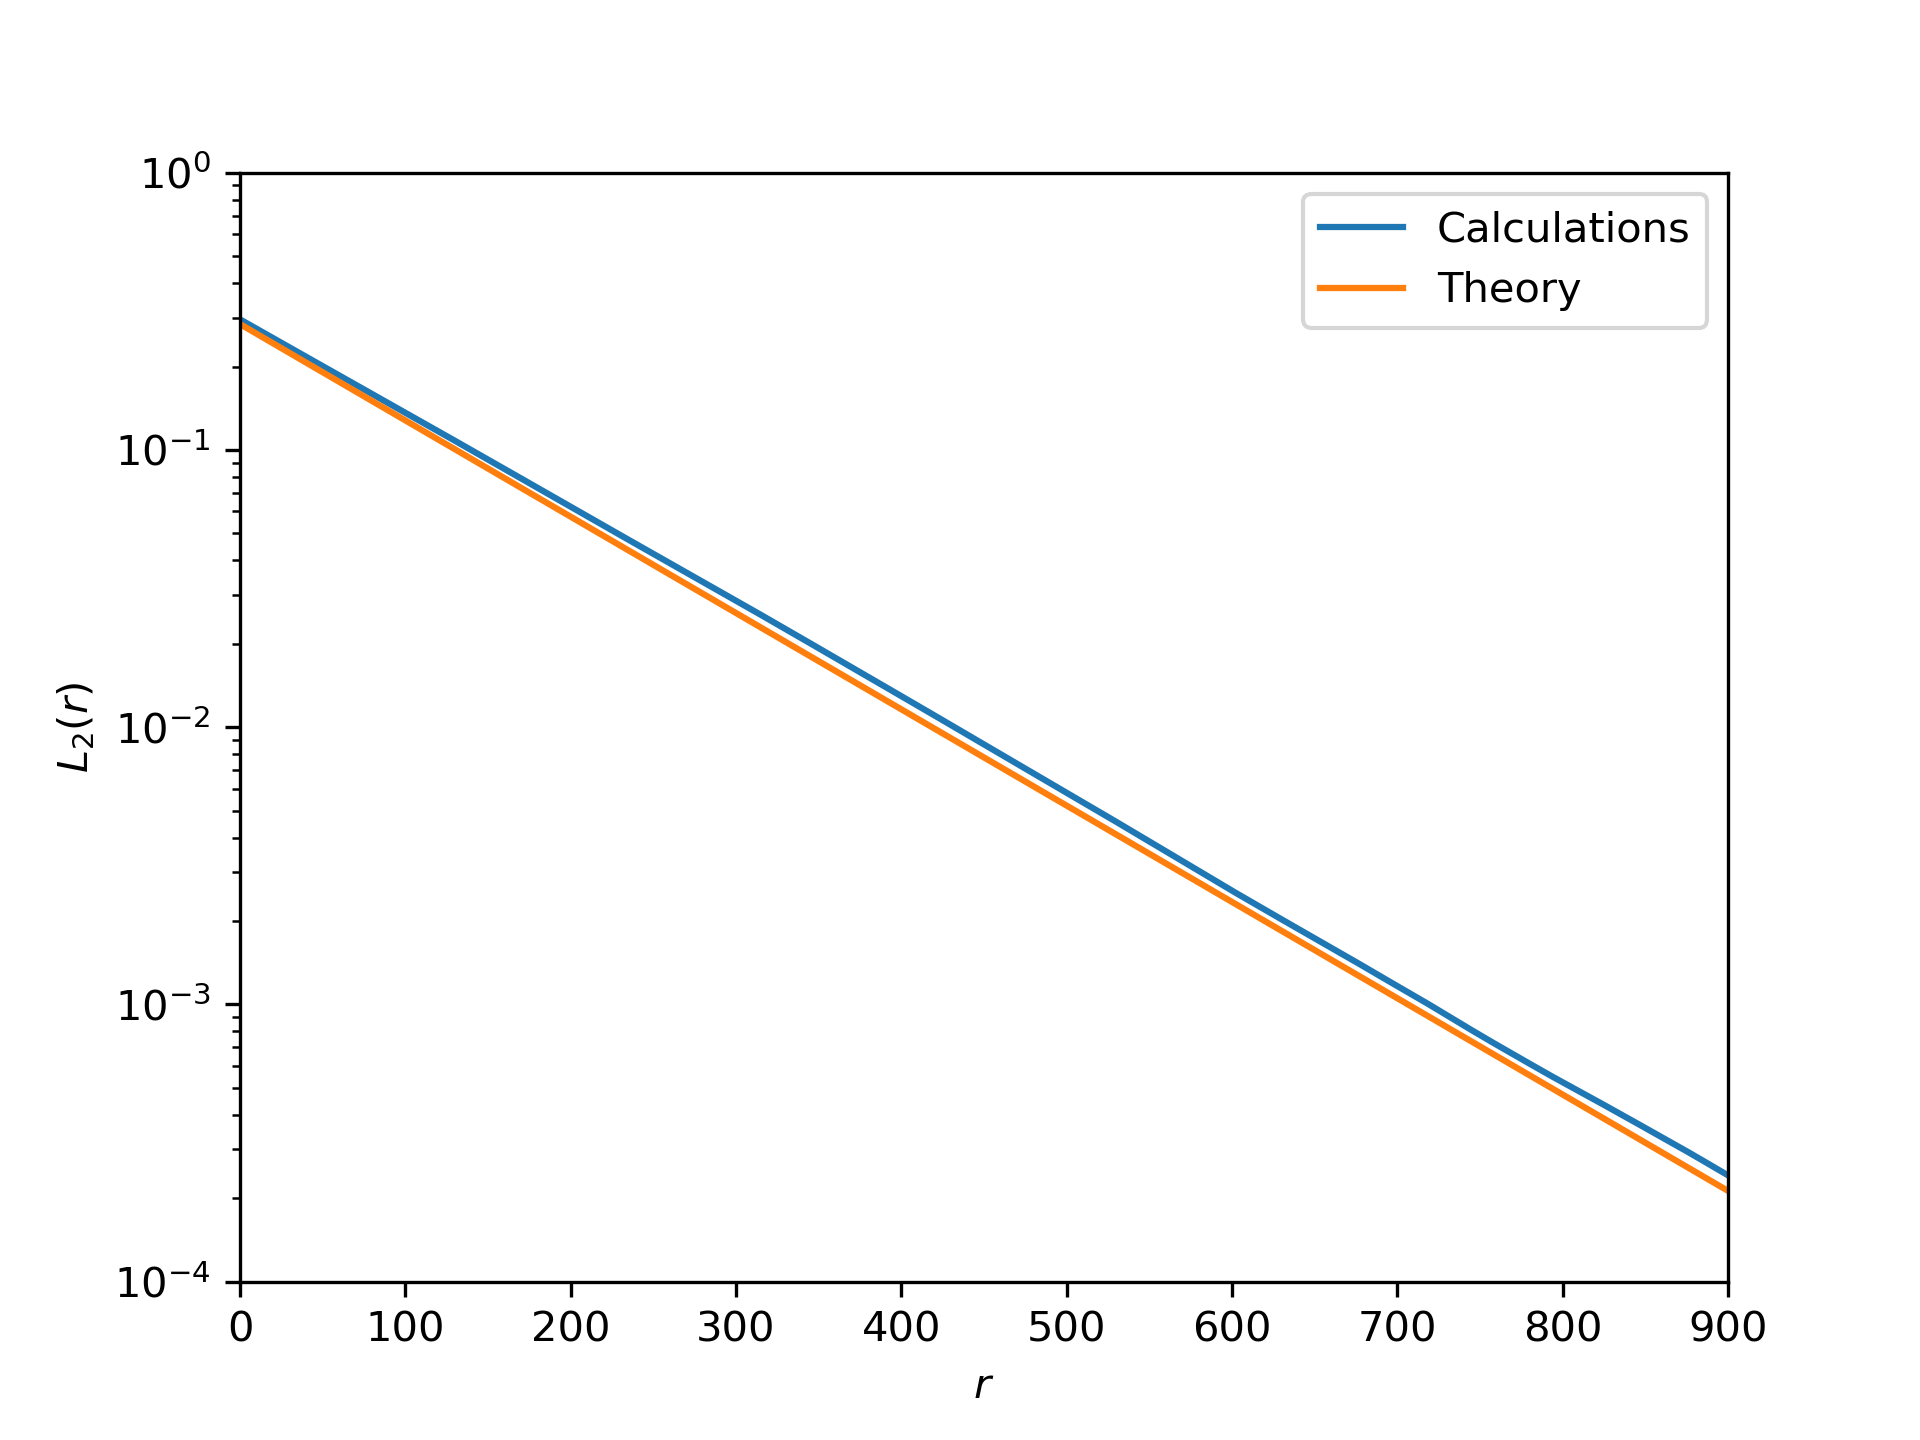
\includegraphics[width=0.475\linewidth]{images/l2-2d.png}
    \label{fig:l2-2d}}
  \hfill
  \subfigure[Two-point correlation function]{
    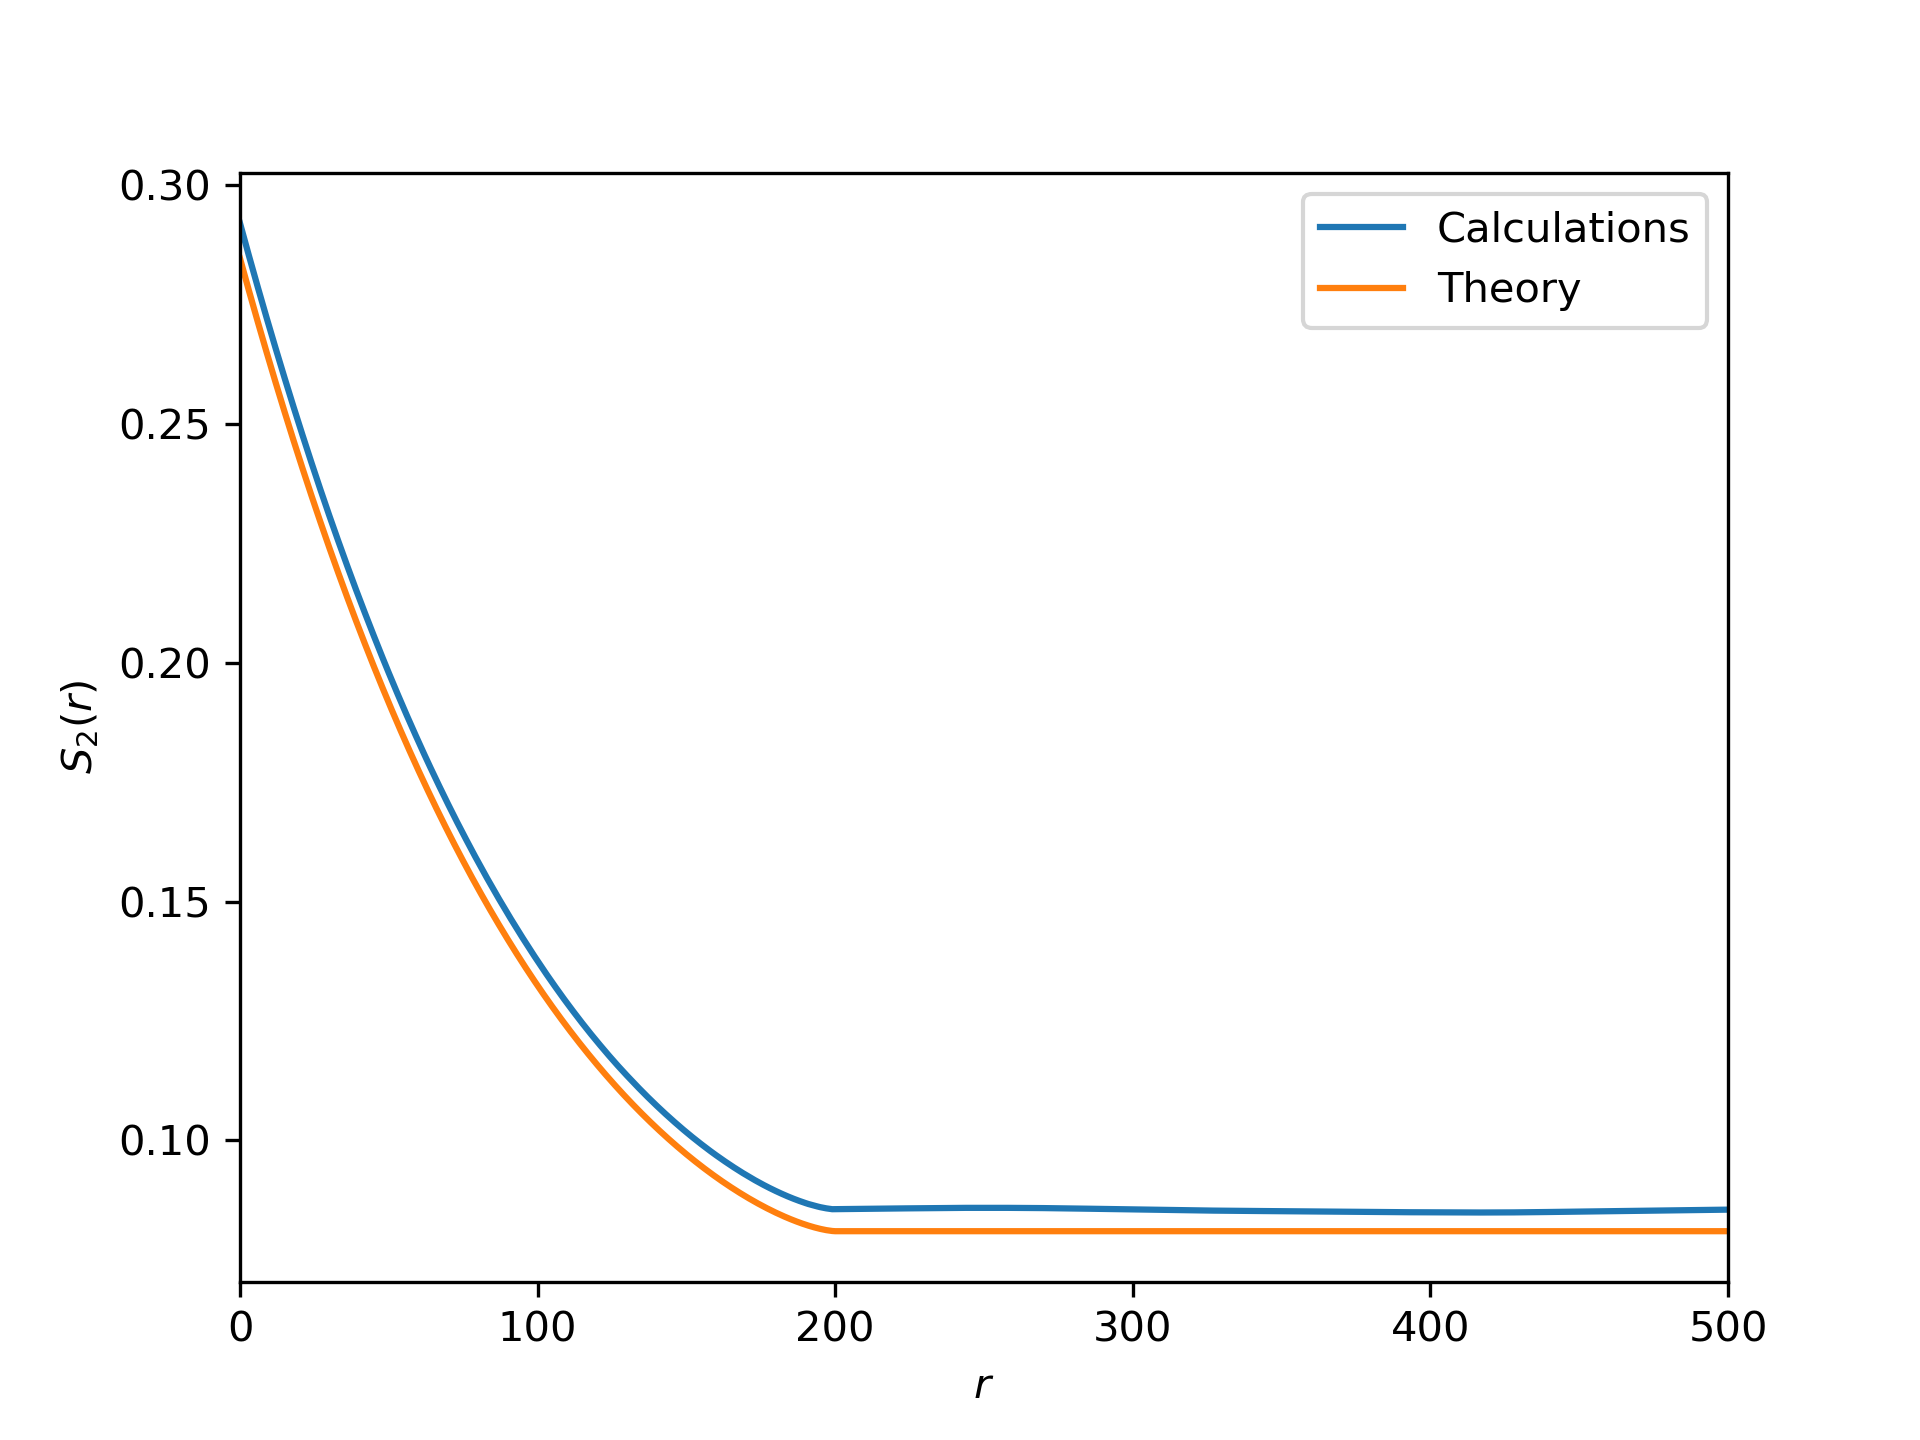
\includegraphics[width=0.475\linewidth]{images/s2-2d.png}
    \label{fig:s2-2d}}
  \vskip\baselineskip
  \subfigure[Surface-surface correlation function]{
    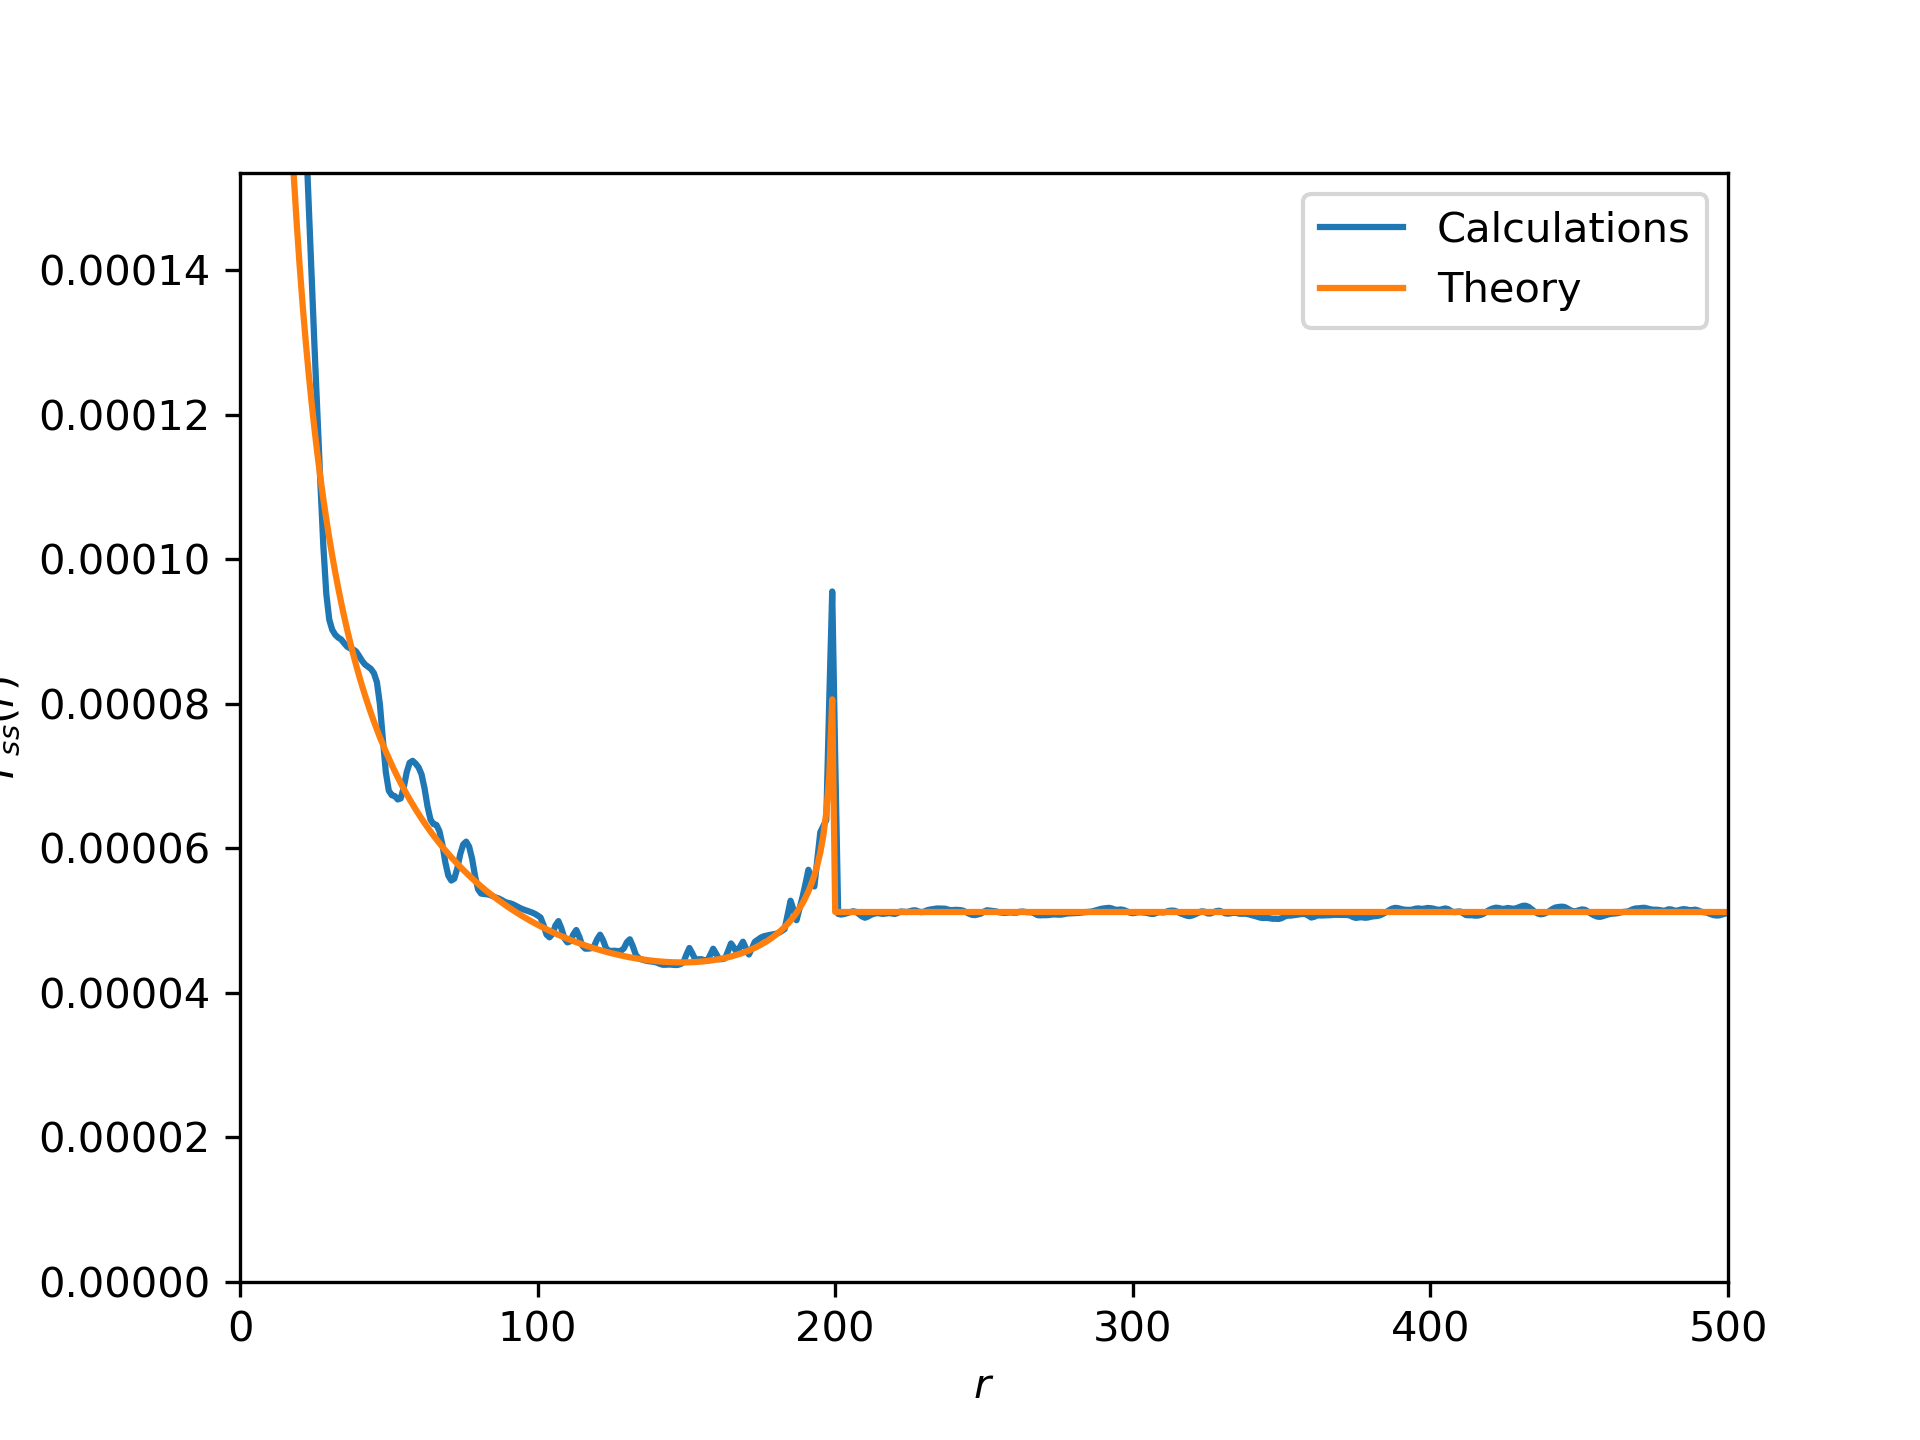
\includegraphics[width=0.475\linewidth]{images/ss-2d.png}
    \label{fig:ss-2d}}
  \hfill
  \subfigure[Surface-void correlation function]{
    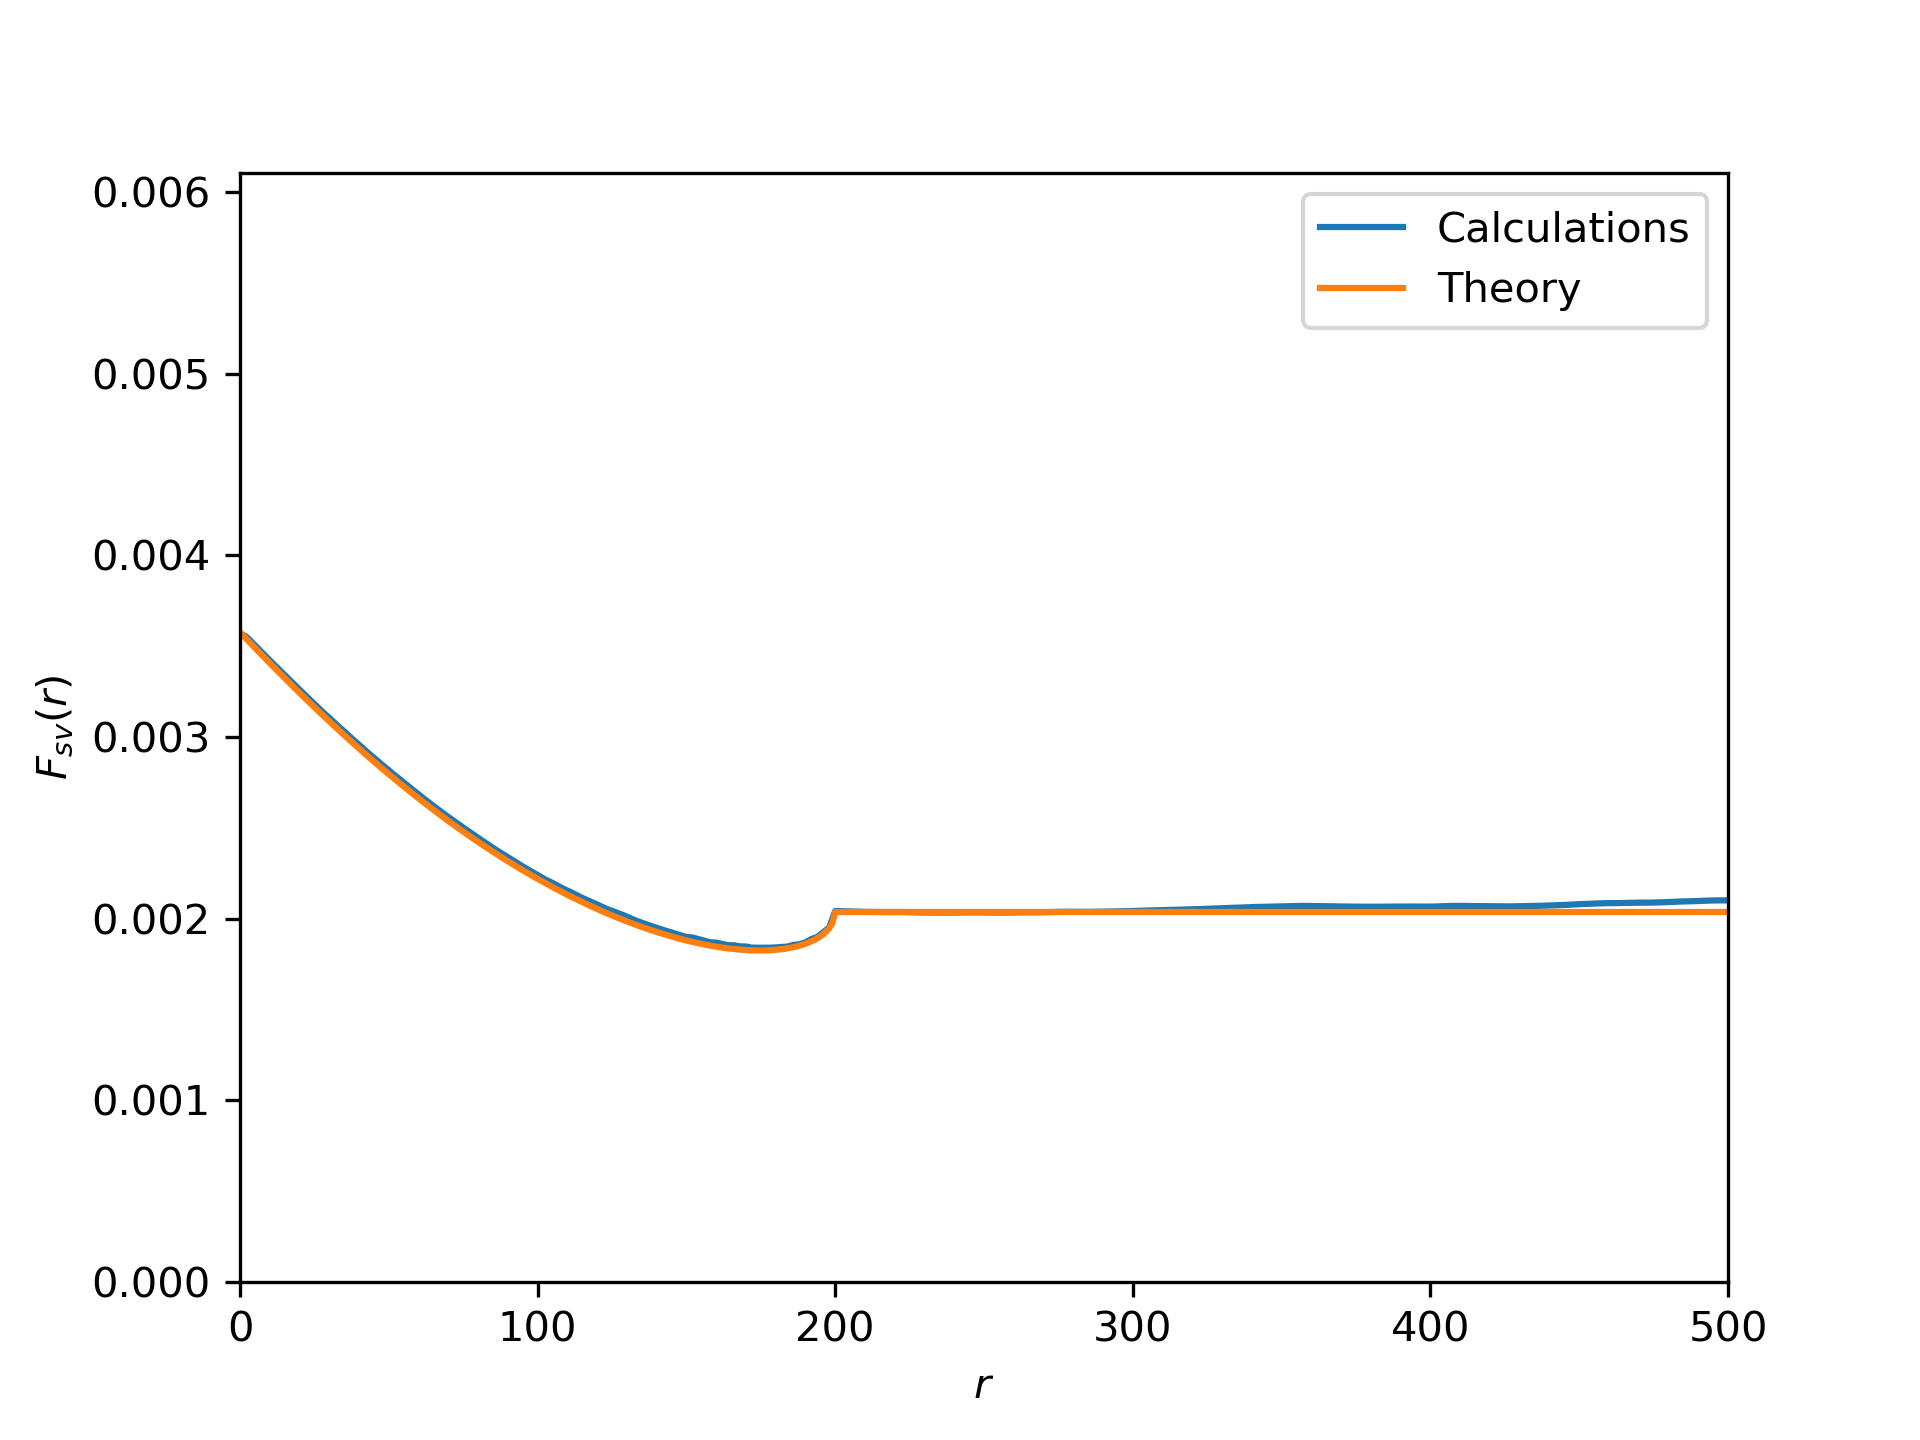
\includegraphics[width=0.475\linewidth]{images/sv-2d.png}
    \label{fig:sv-2d}}
  \caption[]{A comparison of calculated values of $L_2(r)$, $S_2(r)$,
    $F_{ss}(r)$ and $F_{sv}(r)$ with theoretical values for overlapping disks.}
  \label{fig:2d}
\end{figure*}

\begin{figure*}[t]
  \centering
  \subfigure[Lineal-path correlation function]{
    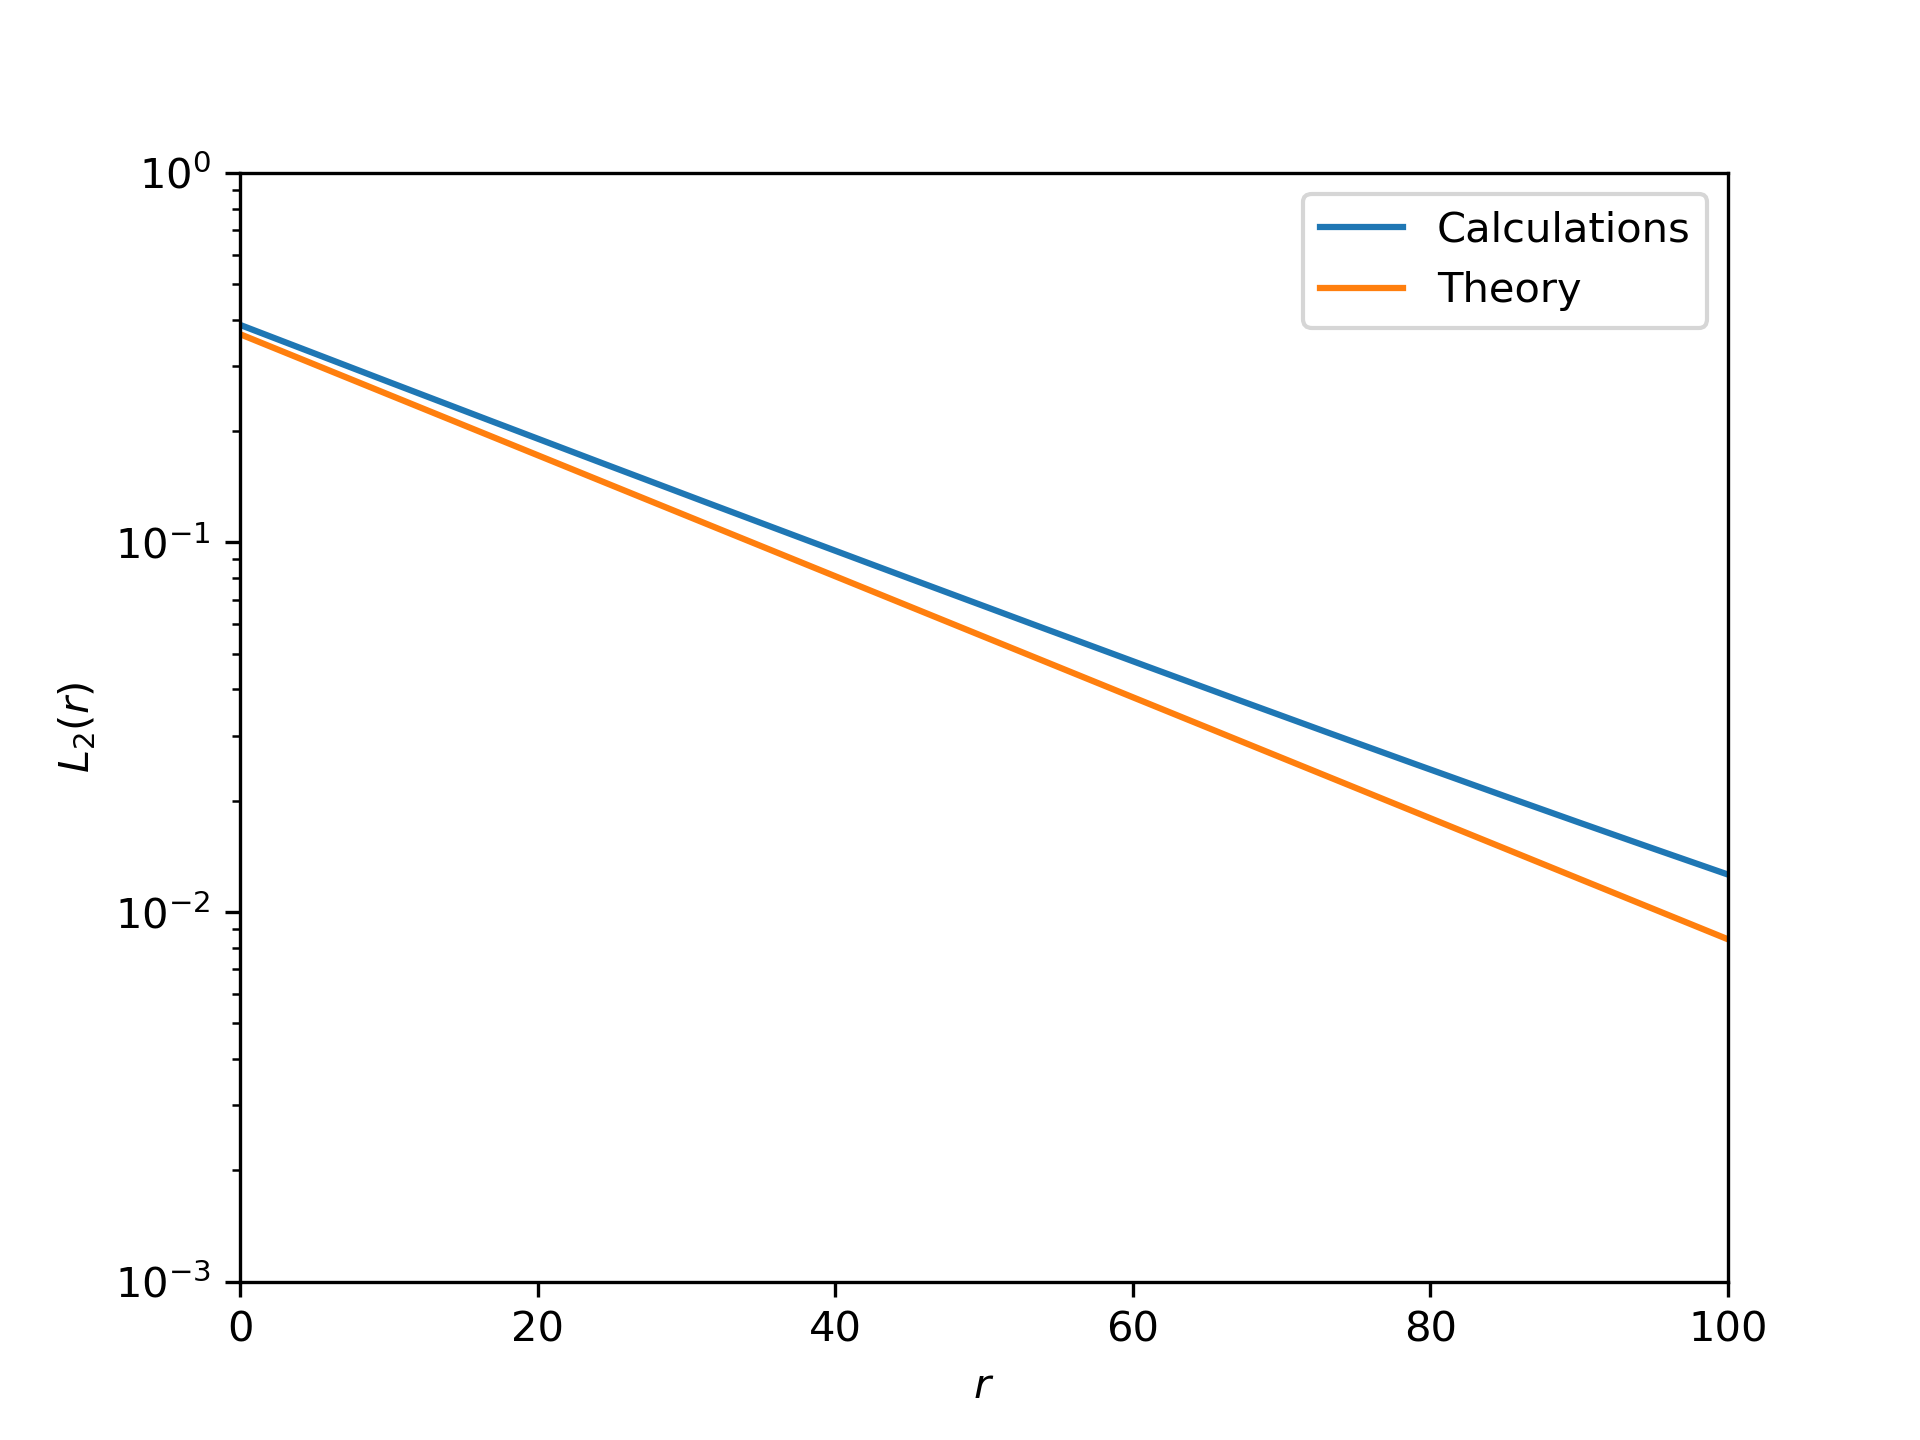
\includegraphics[width=0.475\linewidth]{images/l2-3d.png}
    \label{fig:l2-3d}}
  \hfill
  \subfigure[Two-point correlation function]{
    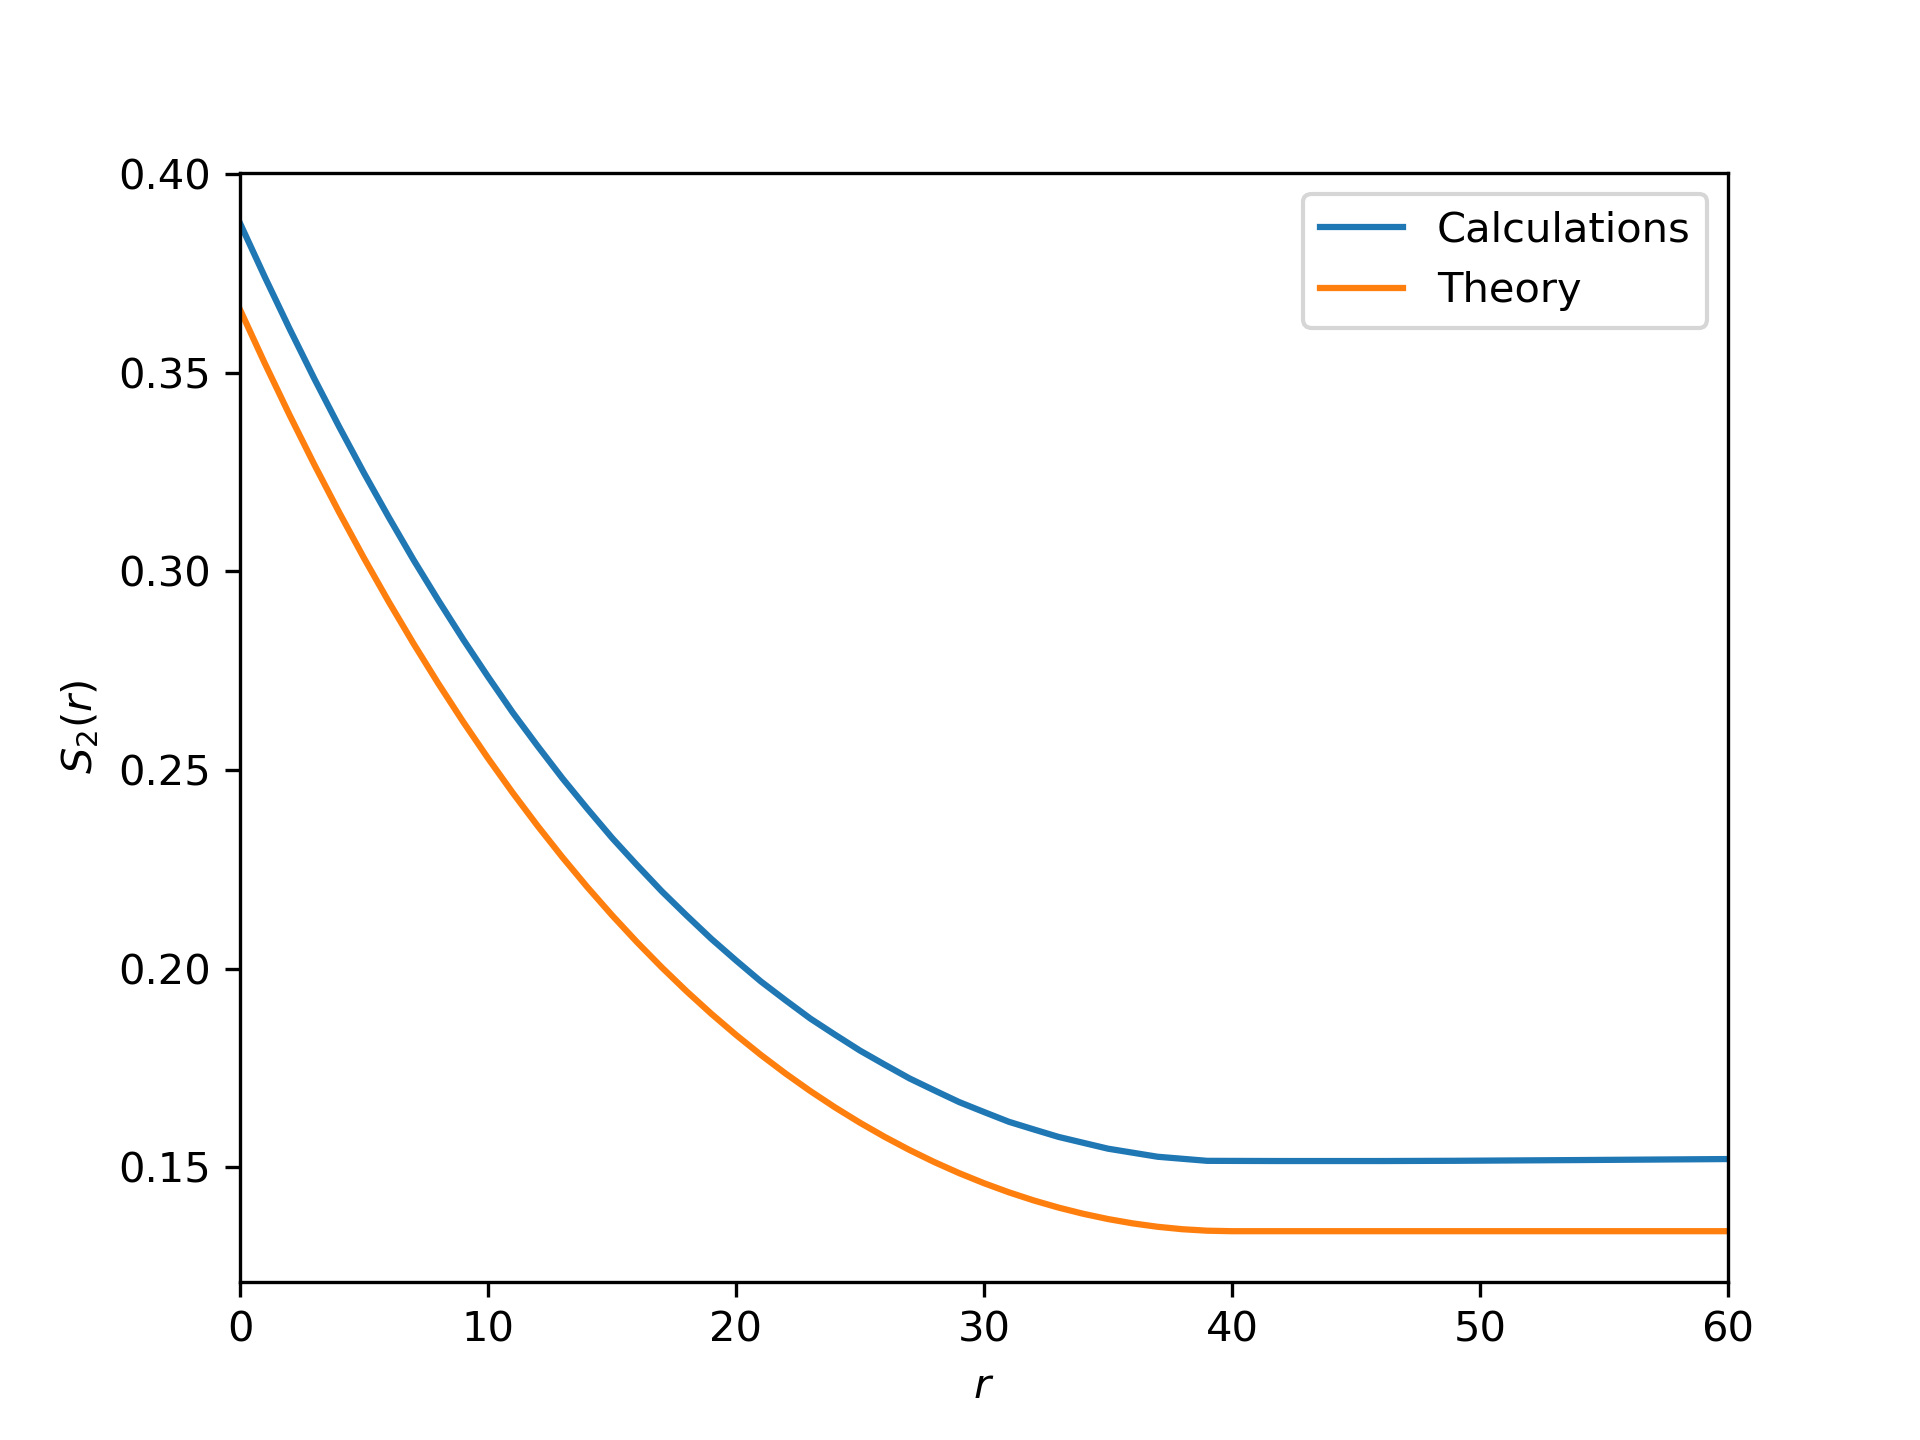
\includegraphics[width=0.475\linewidth]{images/s2-3d.png}
    \label{fig:s3-3d}}
  \vskip\baselineskip
  \subfigure[Surface-surface correlation function]{
    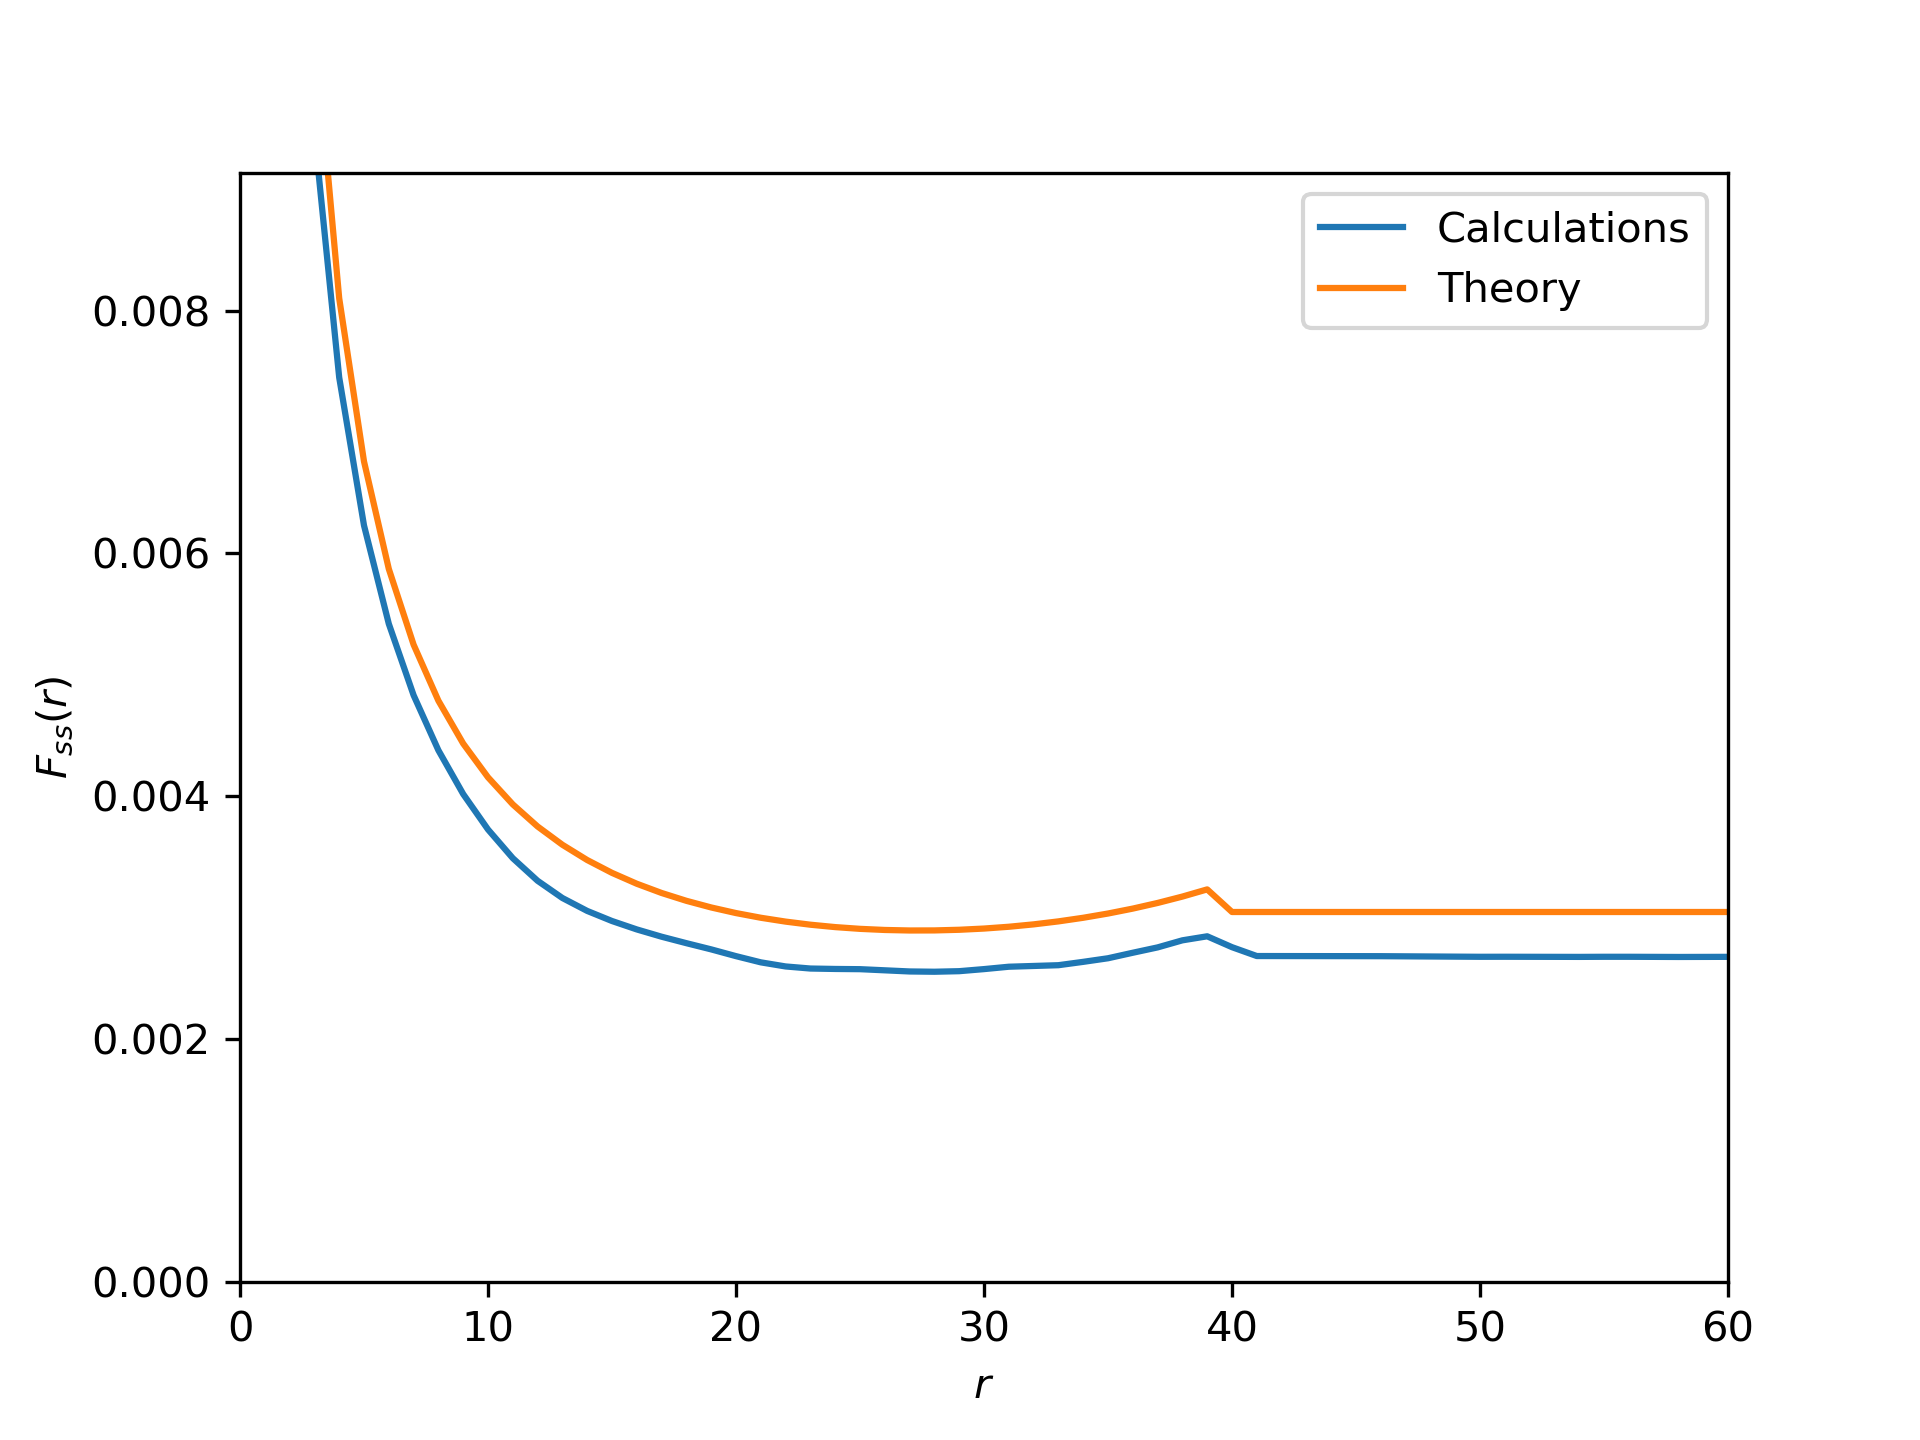
\includegraphics[width=0.475\linewidth]{images/ss-3d.png}
    \label{fig:ss-3d}}
  \hfill
  \subfigure[Surface-void correlation function]{
    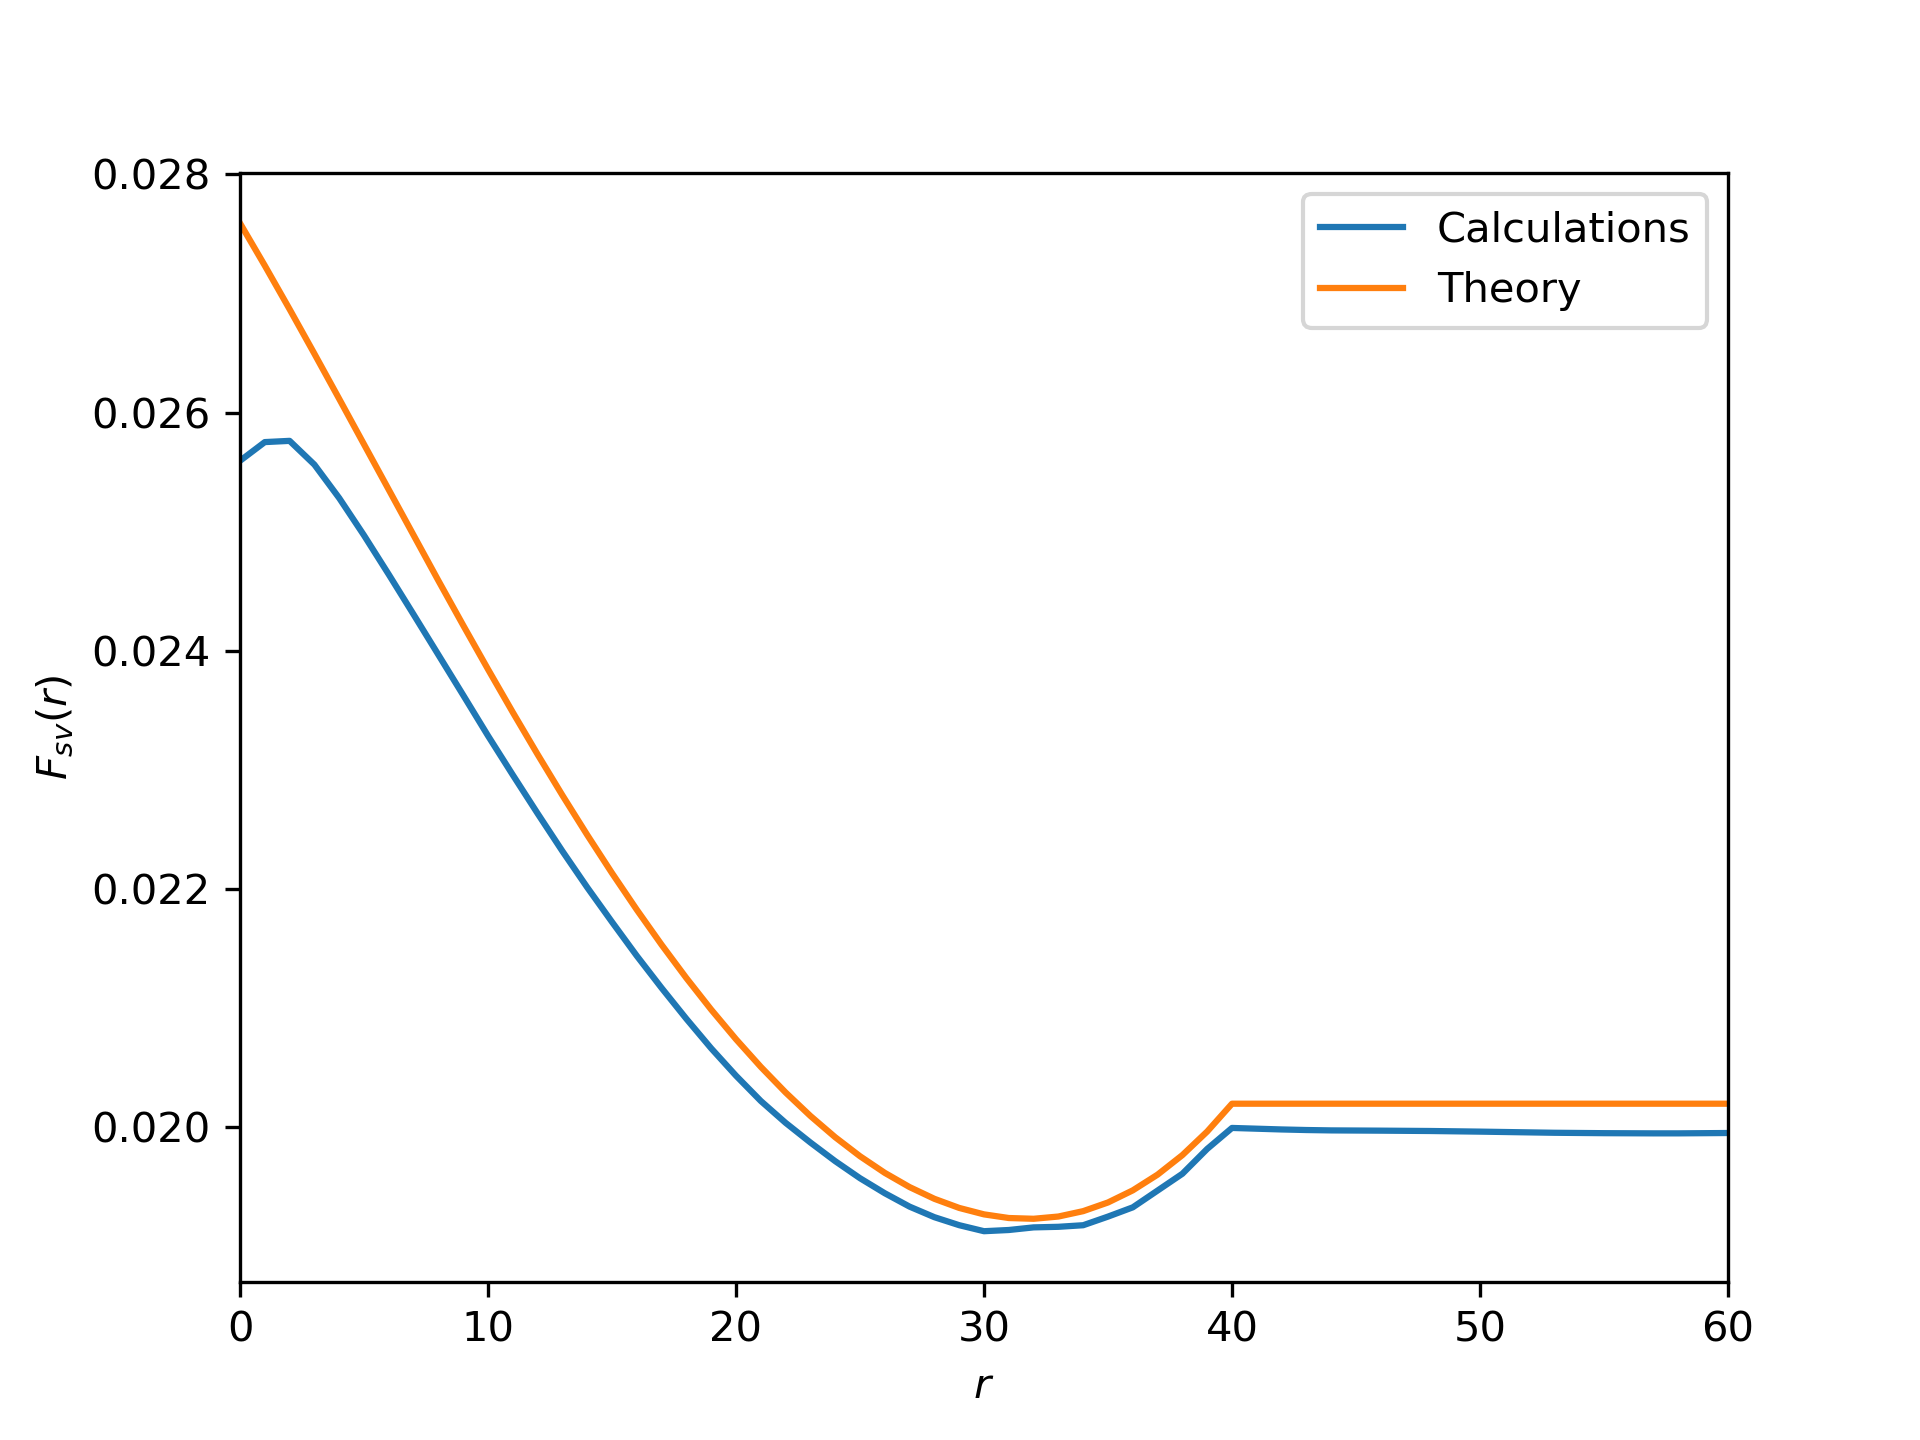
\includegraphics[width=0.475\linewidth]{images/sv-3d.png}
    \label{fig:sv-3d}}
  \caption[]{A comparison of calculated values of $L_2(r)$, $S_2(r)$,
    $F_{ss}(r)$ and $F_{sv}(r)$ with theoretical values for overlapping balls.}
  \label{fig:3d}
\end{figure*}

\begin{figure*}[t]
  \centering
  \subfigure[Pore size correlation function (2D)]{
    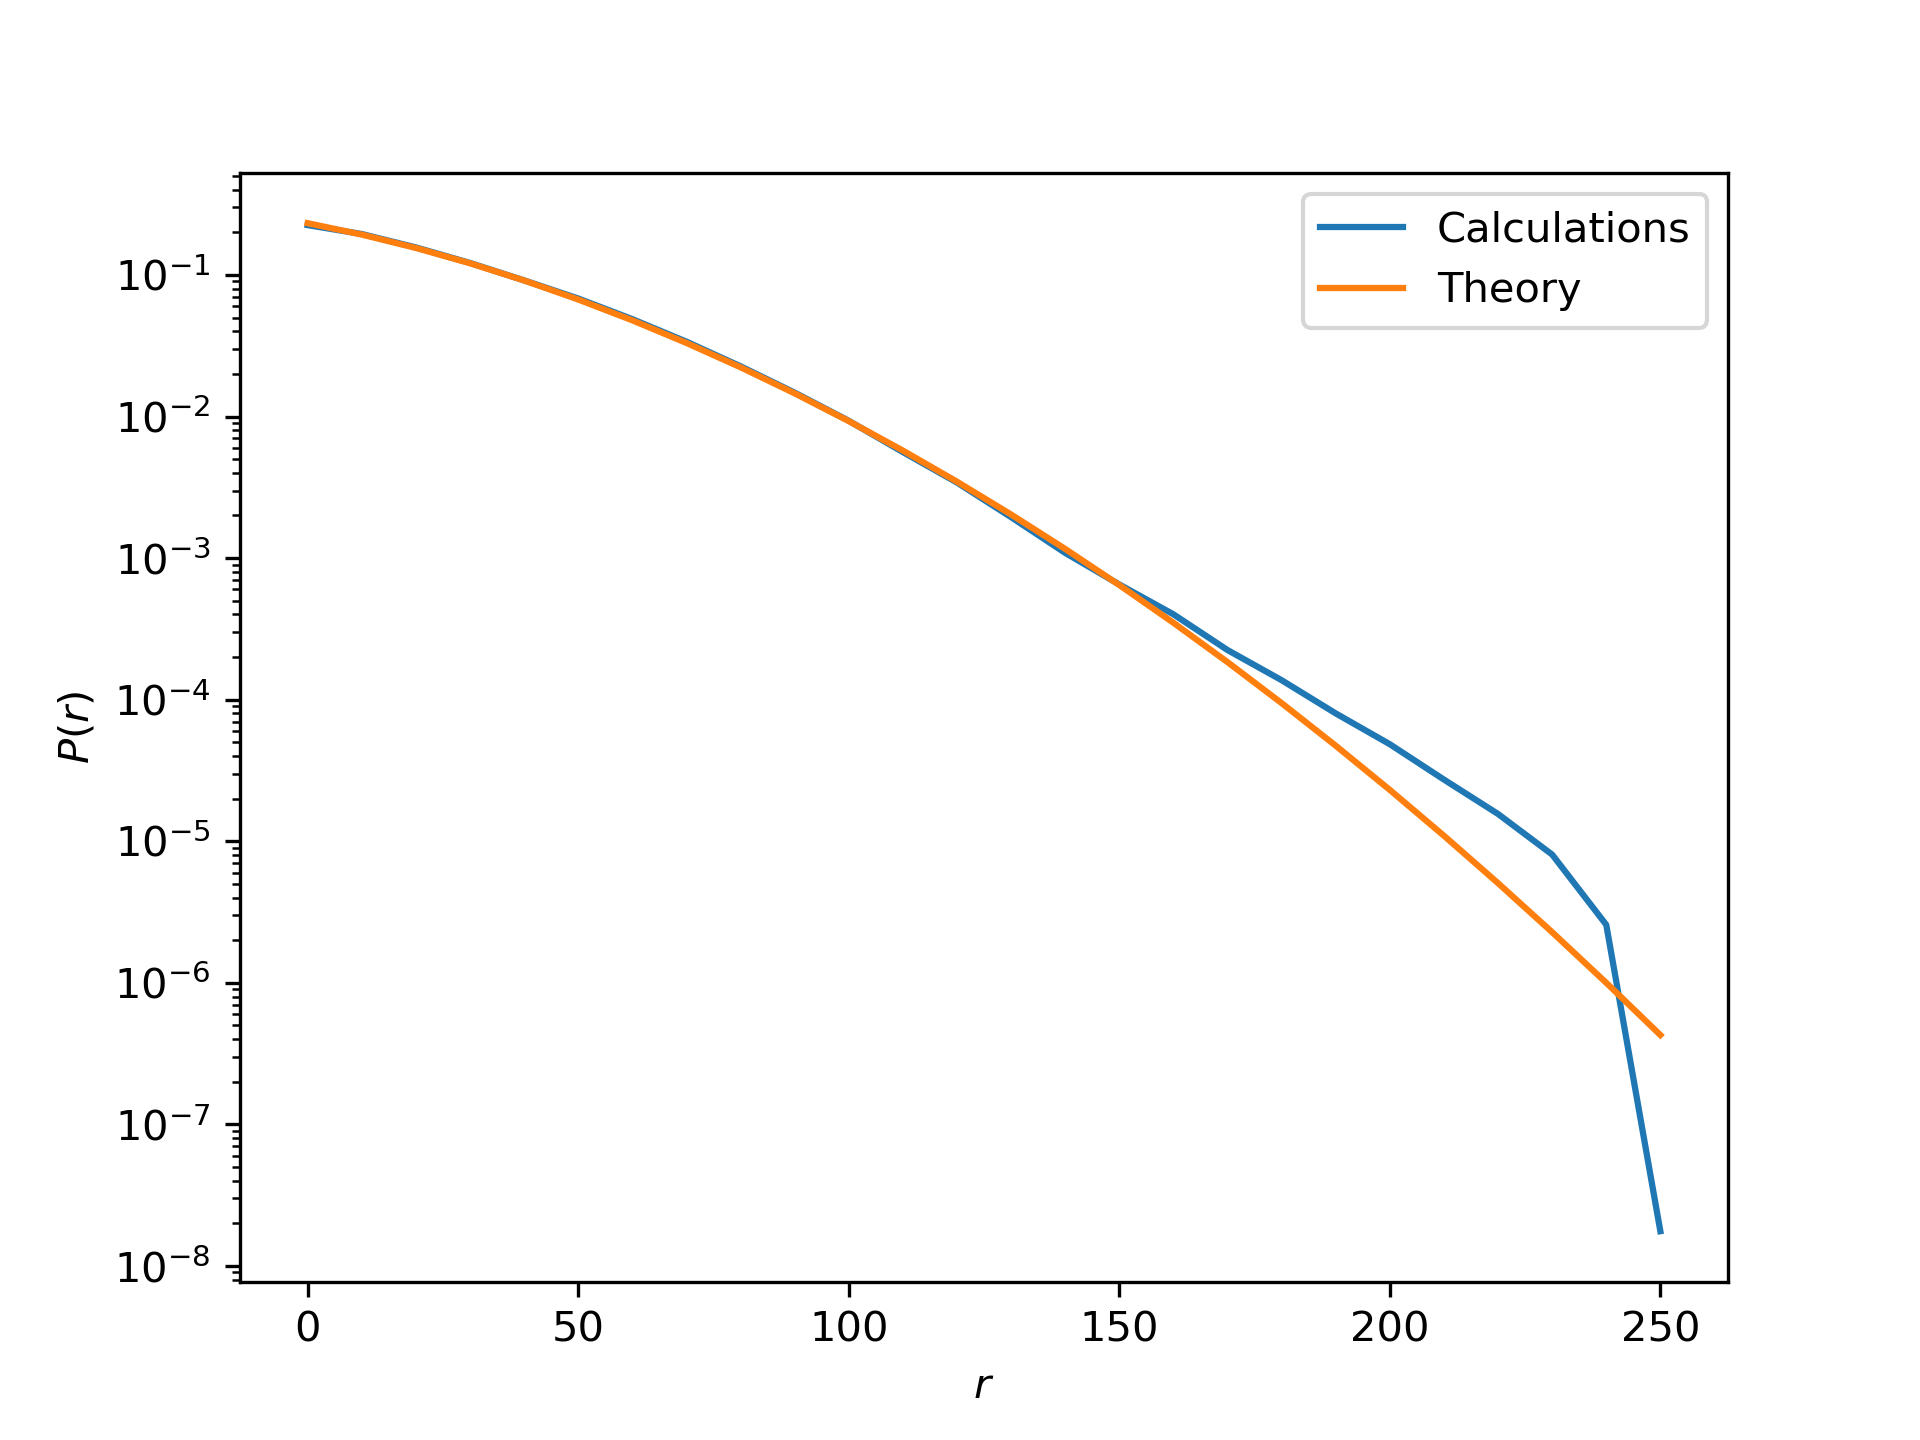
\includegraphics[width=0.475\linewidth]{images/ps-2d.png}
    \label{fig:ps-2d}}
  \hfill
  \subfigure[Chord length correlation function (2D)]{
    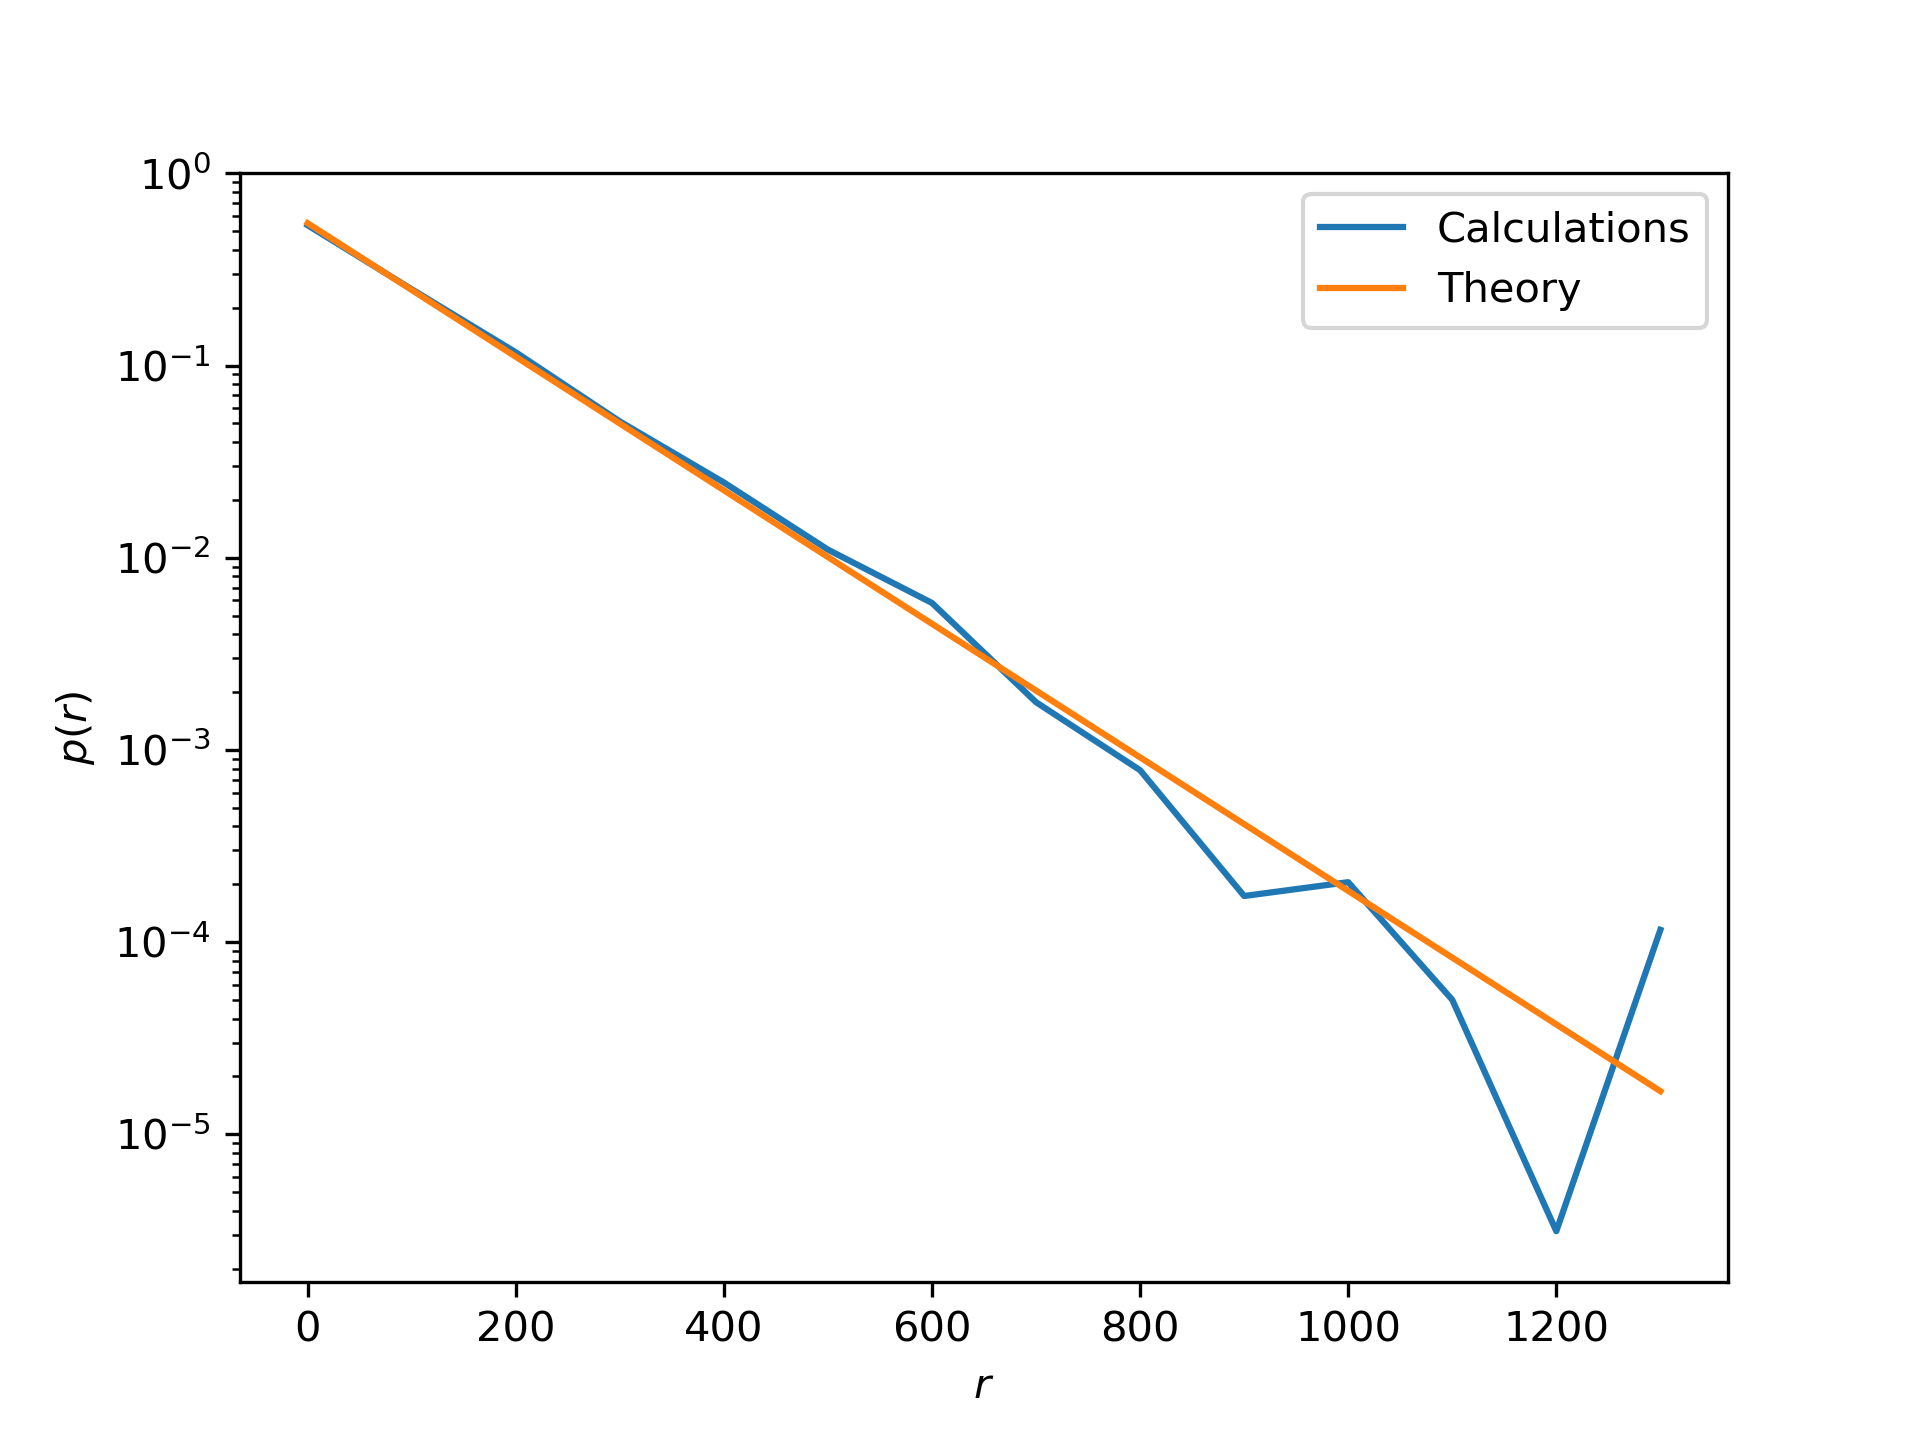
\includegraphics[width=0.475\linewidth]{images/cl-2d.png}
    \label{fig:cl-2d}}
  \vskip\baselineskip
  \subfigure[Pore size correlation function (3D)]{
    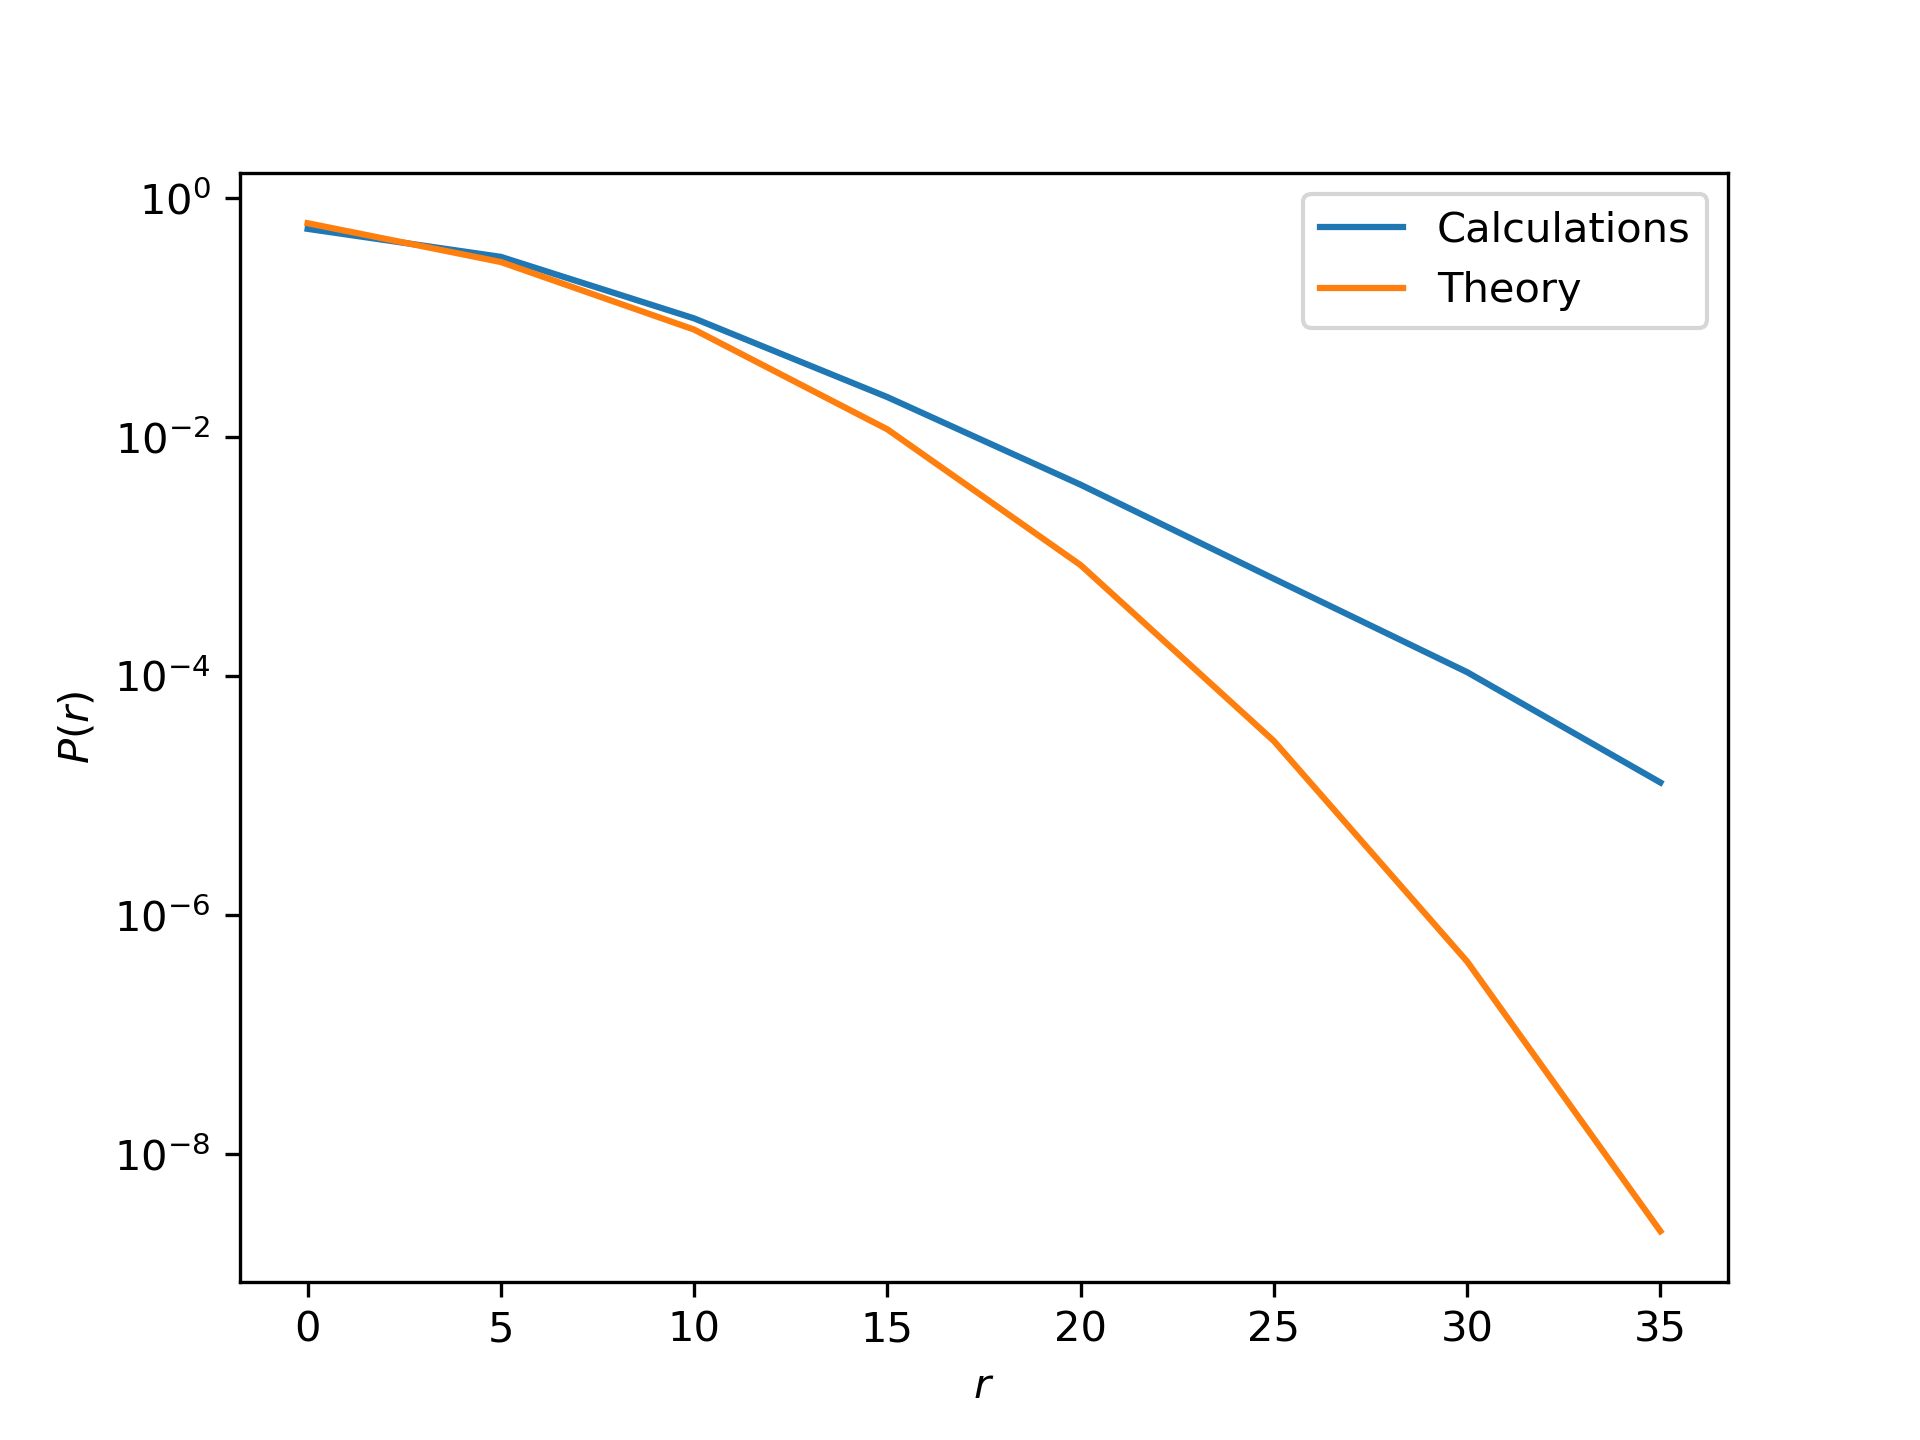
\includegraphics[width=0.475\linewidth]{images/ps-3d.png}
    \label{fig:ps-3d}}
  \hfill
  \subfigure[Chord length correlation function (3D)]{
    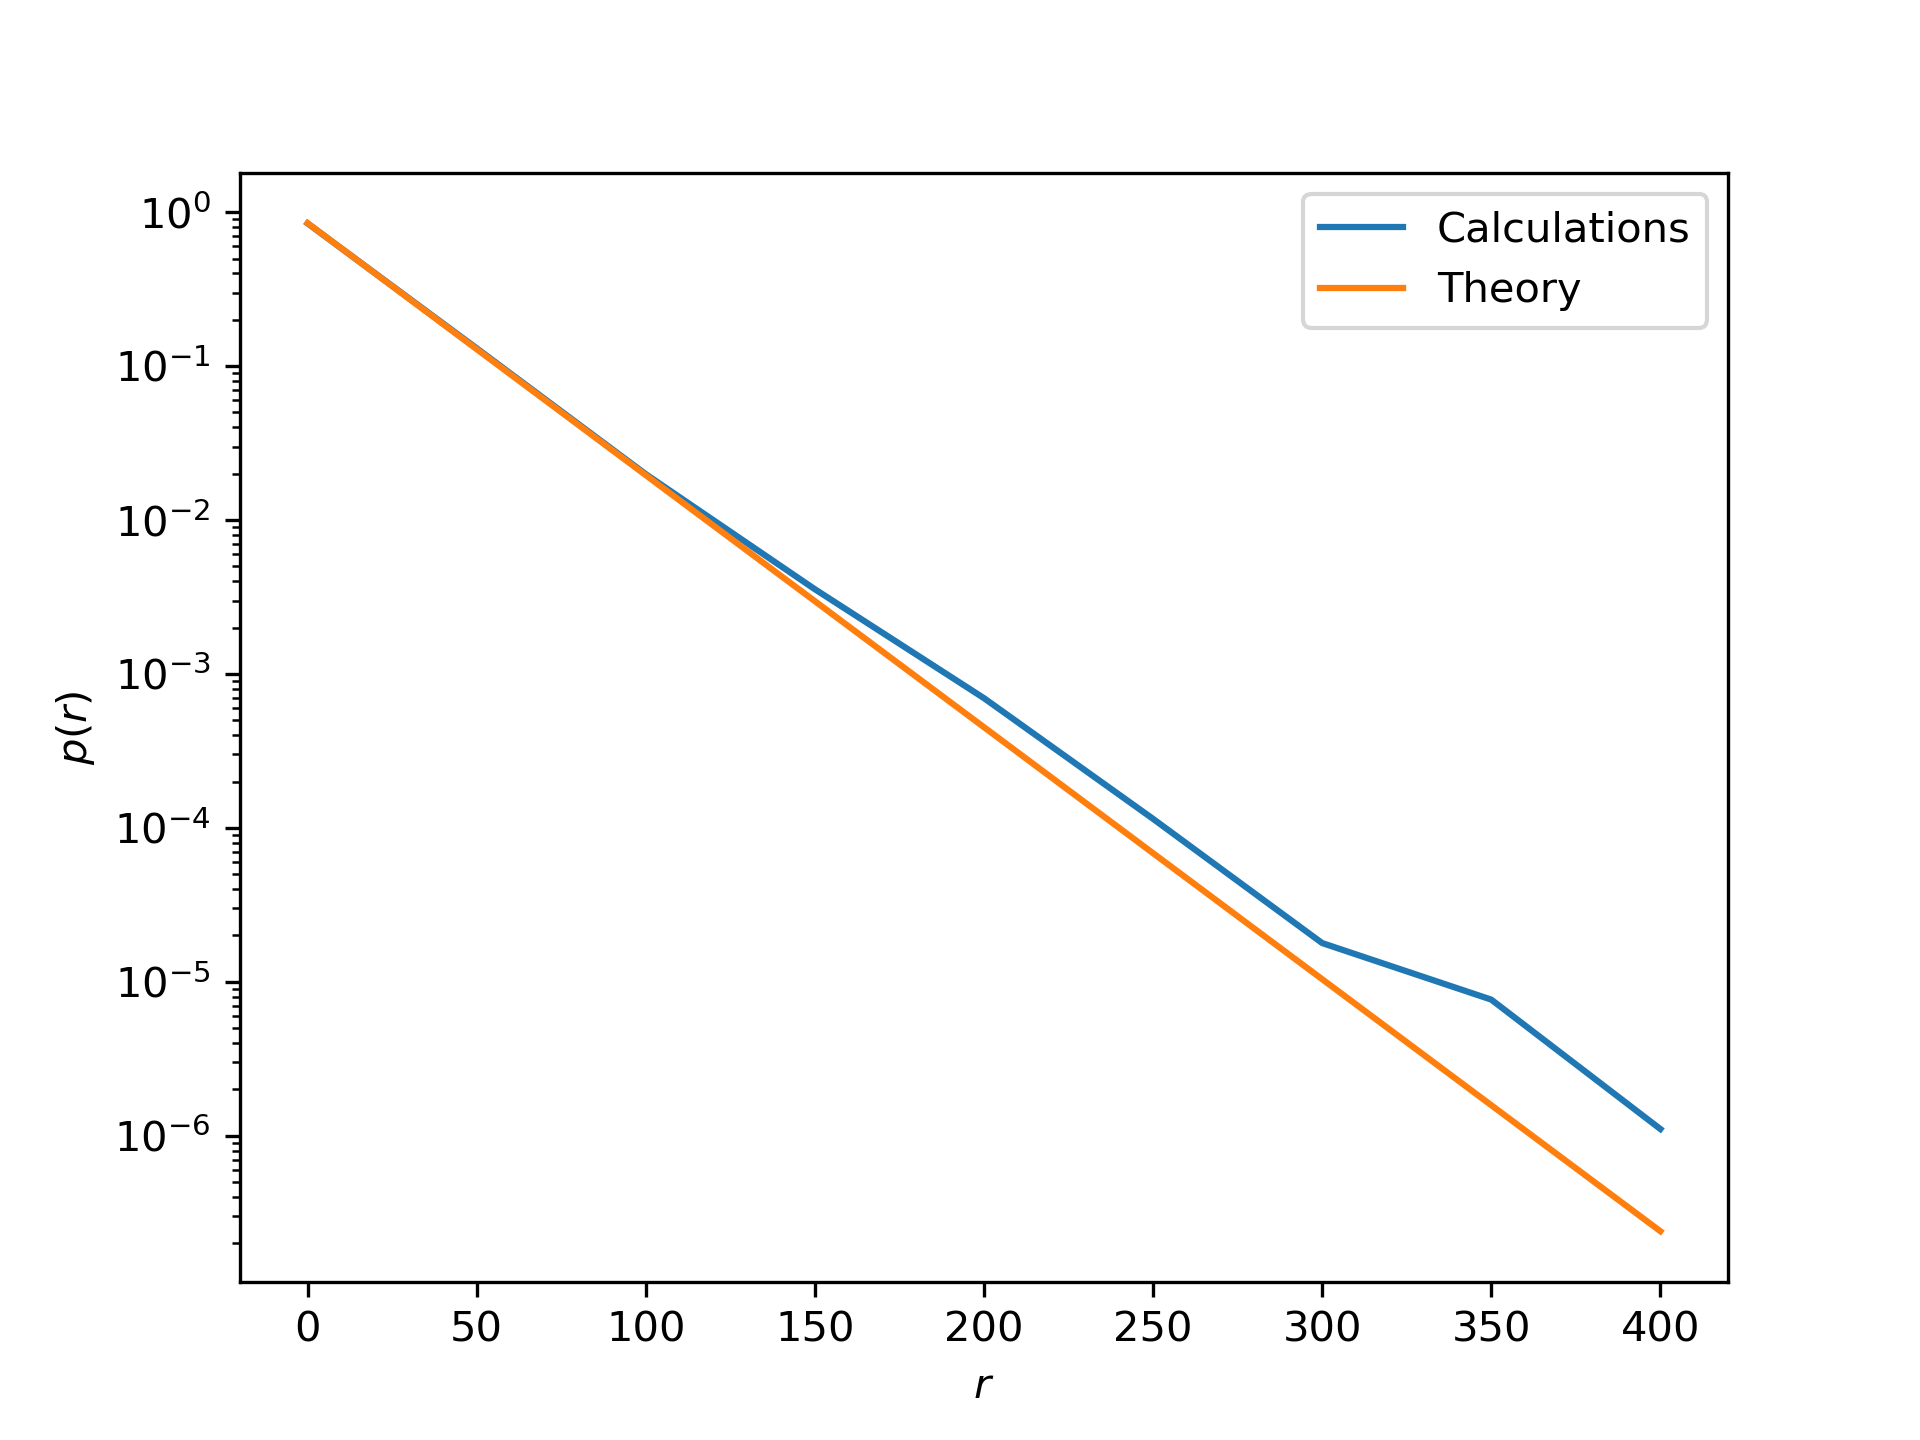
\includegraphics[width=0.475\linewidth]{images/cl-3d.png}
    \label{fig:cl-3d}}
  \caption[]{A comparison of calculated values of $P(r)$ and $p(r)$
    with theoretical values for overlapping disks (\cref{fig:ps-2d} and
    \cref{fig:cl-2d}) and balls(\cref{fig:ps-3d} and \cref{fig:cl-3d}).}
  \label{fig:pscl}
\end{figure*}

\section{Efficiency of our algorithms}
\label{sec:efficiency}
To measure efficiecy of our algorithms we use a machine with the following
configuration:
\begin{itemize}
\item \textbf{CPU}: AMD Ryzen 5 1600X
\item \textbf{Memory}: 32~Gb DDR4-2400 memory
\item \textbf{GPU}: Nvidia Tesla V100 with 32~Gb video memory
\end{itemize}

We generate two (resp. three) dimensional square (resp. cubic) binary arrays
with different number of elements. Each element $a_{ij}$ (resp. $a_{ijk}$) of a
two-dimensional (resp. three-dimensional) array is calculated as follows:
\begin{align*}
  a_{ij} & = \left\{
  \begin{array}{ll}
    0 & \quad vn(5i/s, 5j/s, 0, 5, 34365) < 0.5 \\
    1 & \quad \text{otherwise}
  \end{array}
  \right. \\
  a_{ijk} & = \left\{
  \begin{array}{ll}
    0 & \quad vn(5i/s, 5j/s, 5k/s, 5, 34365) < 0.5 \\
    1 & \quad \text{otherwise}
  \end{array}
  \right.
\end{align*}
Here $vn(x,y,z,o,s)$ is a value noise function. We fix a number of
octaves $o = 5$ and a random seed $s = 34365$. The particular implementation of
value noise for our measurements was taken from \code{ValueNoise.jl} package. An
example of a two-dimensional image generated in this way is on
\cref{fig:valuenoise}.

To measure efficiency of \code{Directional} module we generate ten arrays with
a side of a square $s = 1000, 2000, \dots, 10000$ pixels for two-dimensional
case and ten arrays with a side of a cube $s = 50, 100, \dots, 500$ voxels for
three-dimensional case and calculate execution time for each function. All
functions are calculated with default values of optional arguments (that is:
closed walls boundary conditions and computation along axial directions).

With the \code{Map} module we follow the same procedure. Many functions in
\code{Map} can utilize Nvidia's GPUs using the CUDA library. For example,
two-point correlation function uses FFT transform optimized for Nvidia GPUs and
provided in \code{CUDA.FFT} package. We provide execution times for both CPU and
GPU. The choice between CPU or GPU version is made depending on type of input
array. If it's \code{CuArray} rather than generic \code{AbstractArray} then CUDA
implementation is chosen. Please note, that CPU versions are much slower, so we
choose a different sides of squares ($s = 700, 1350, \dots, 7000$) and cubes
($s = 10, 45, \dots, 350$) for evaluation of the performance.

The measurements of execution time is on \cref{fig:timings}. As you can see, GPU
versions (when available) are faster than CPU versions and limited only by
amount of video memory. Functions in \code{Directional} are slower (with
exception of the lineal-path function) but are also useful in medium
reconstruction algorithms which utilize simulated annealing.

\begin{figure}[ht]
  \centering
  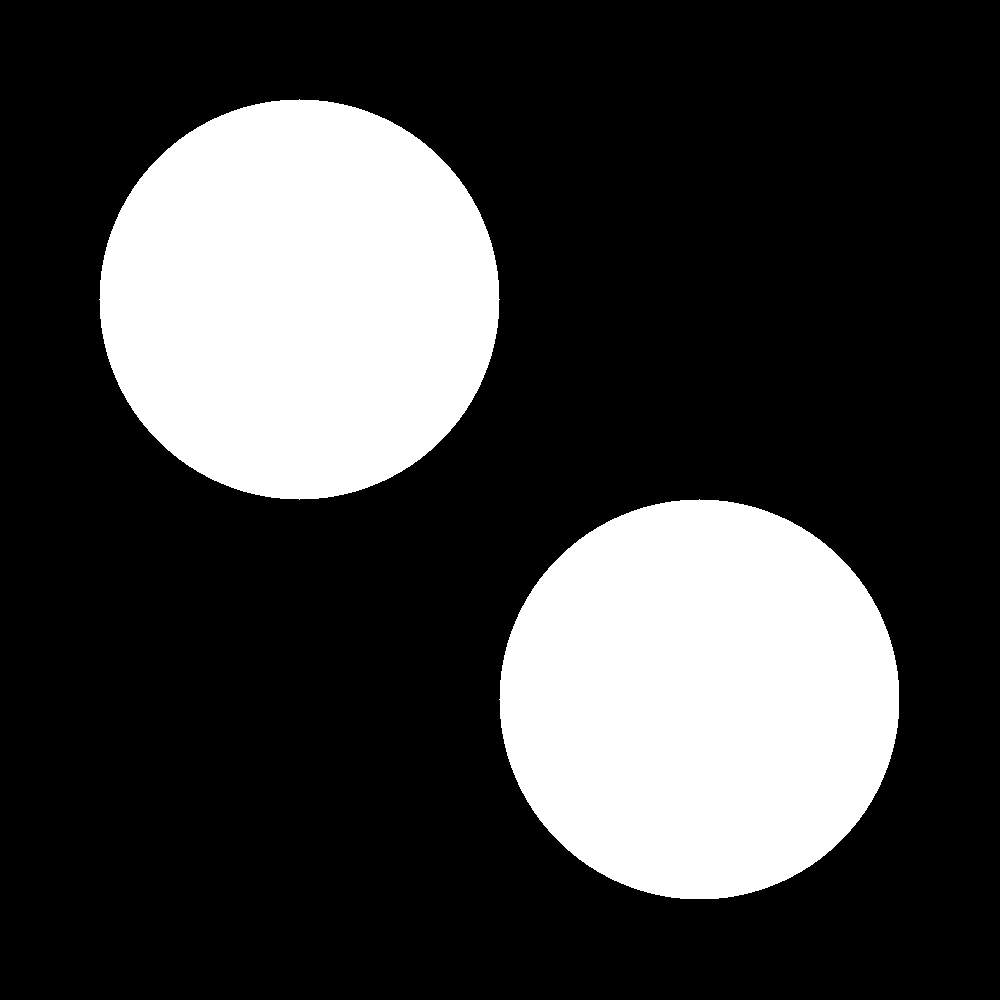
\includegraphics[width=0.9\linewidth]{images/timing-image.png}
  \caption[]{An example of 2D image used in timing measurements.}
  \label{fig:valuenoise}
\end{figure}

\begin{figure*}[t]
  \centering
  \subfigure[Two-dimensional case, module \code{Directional}]{
    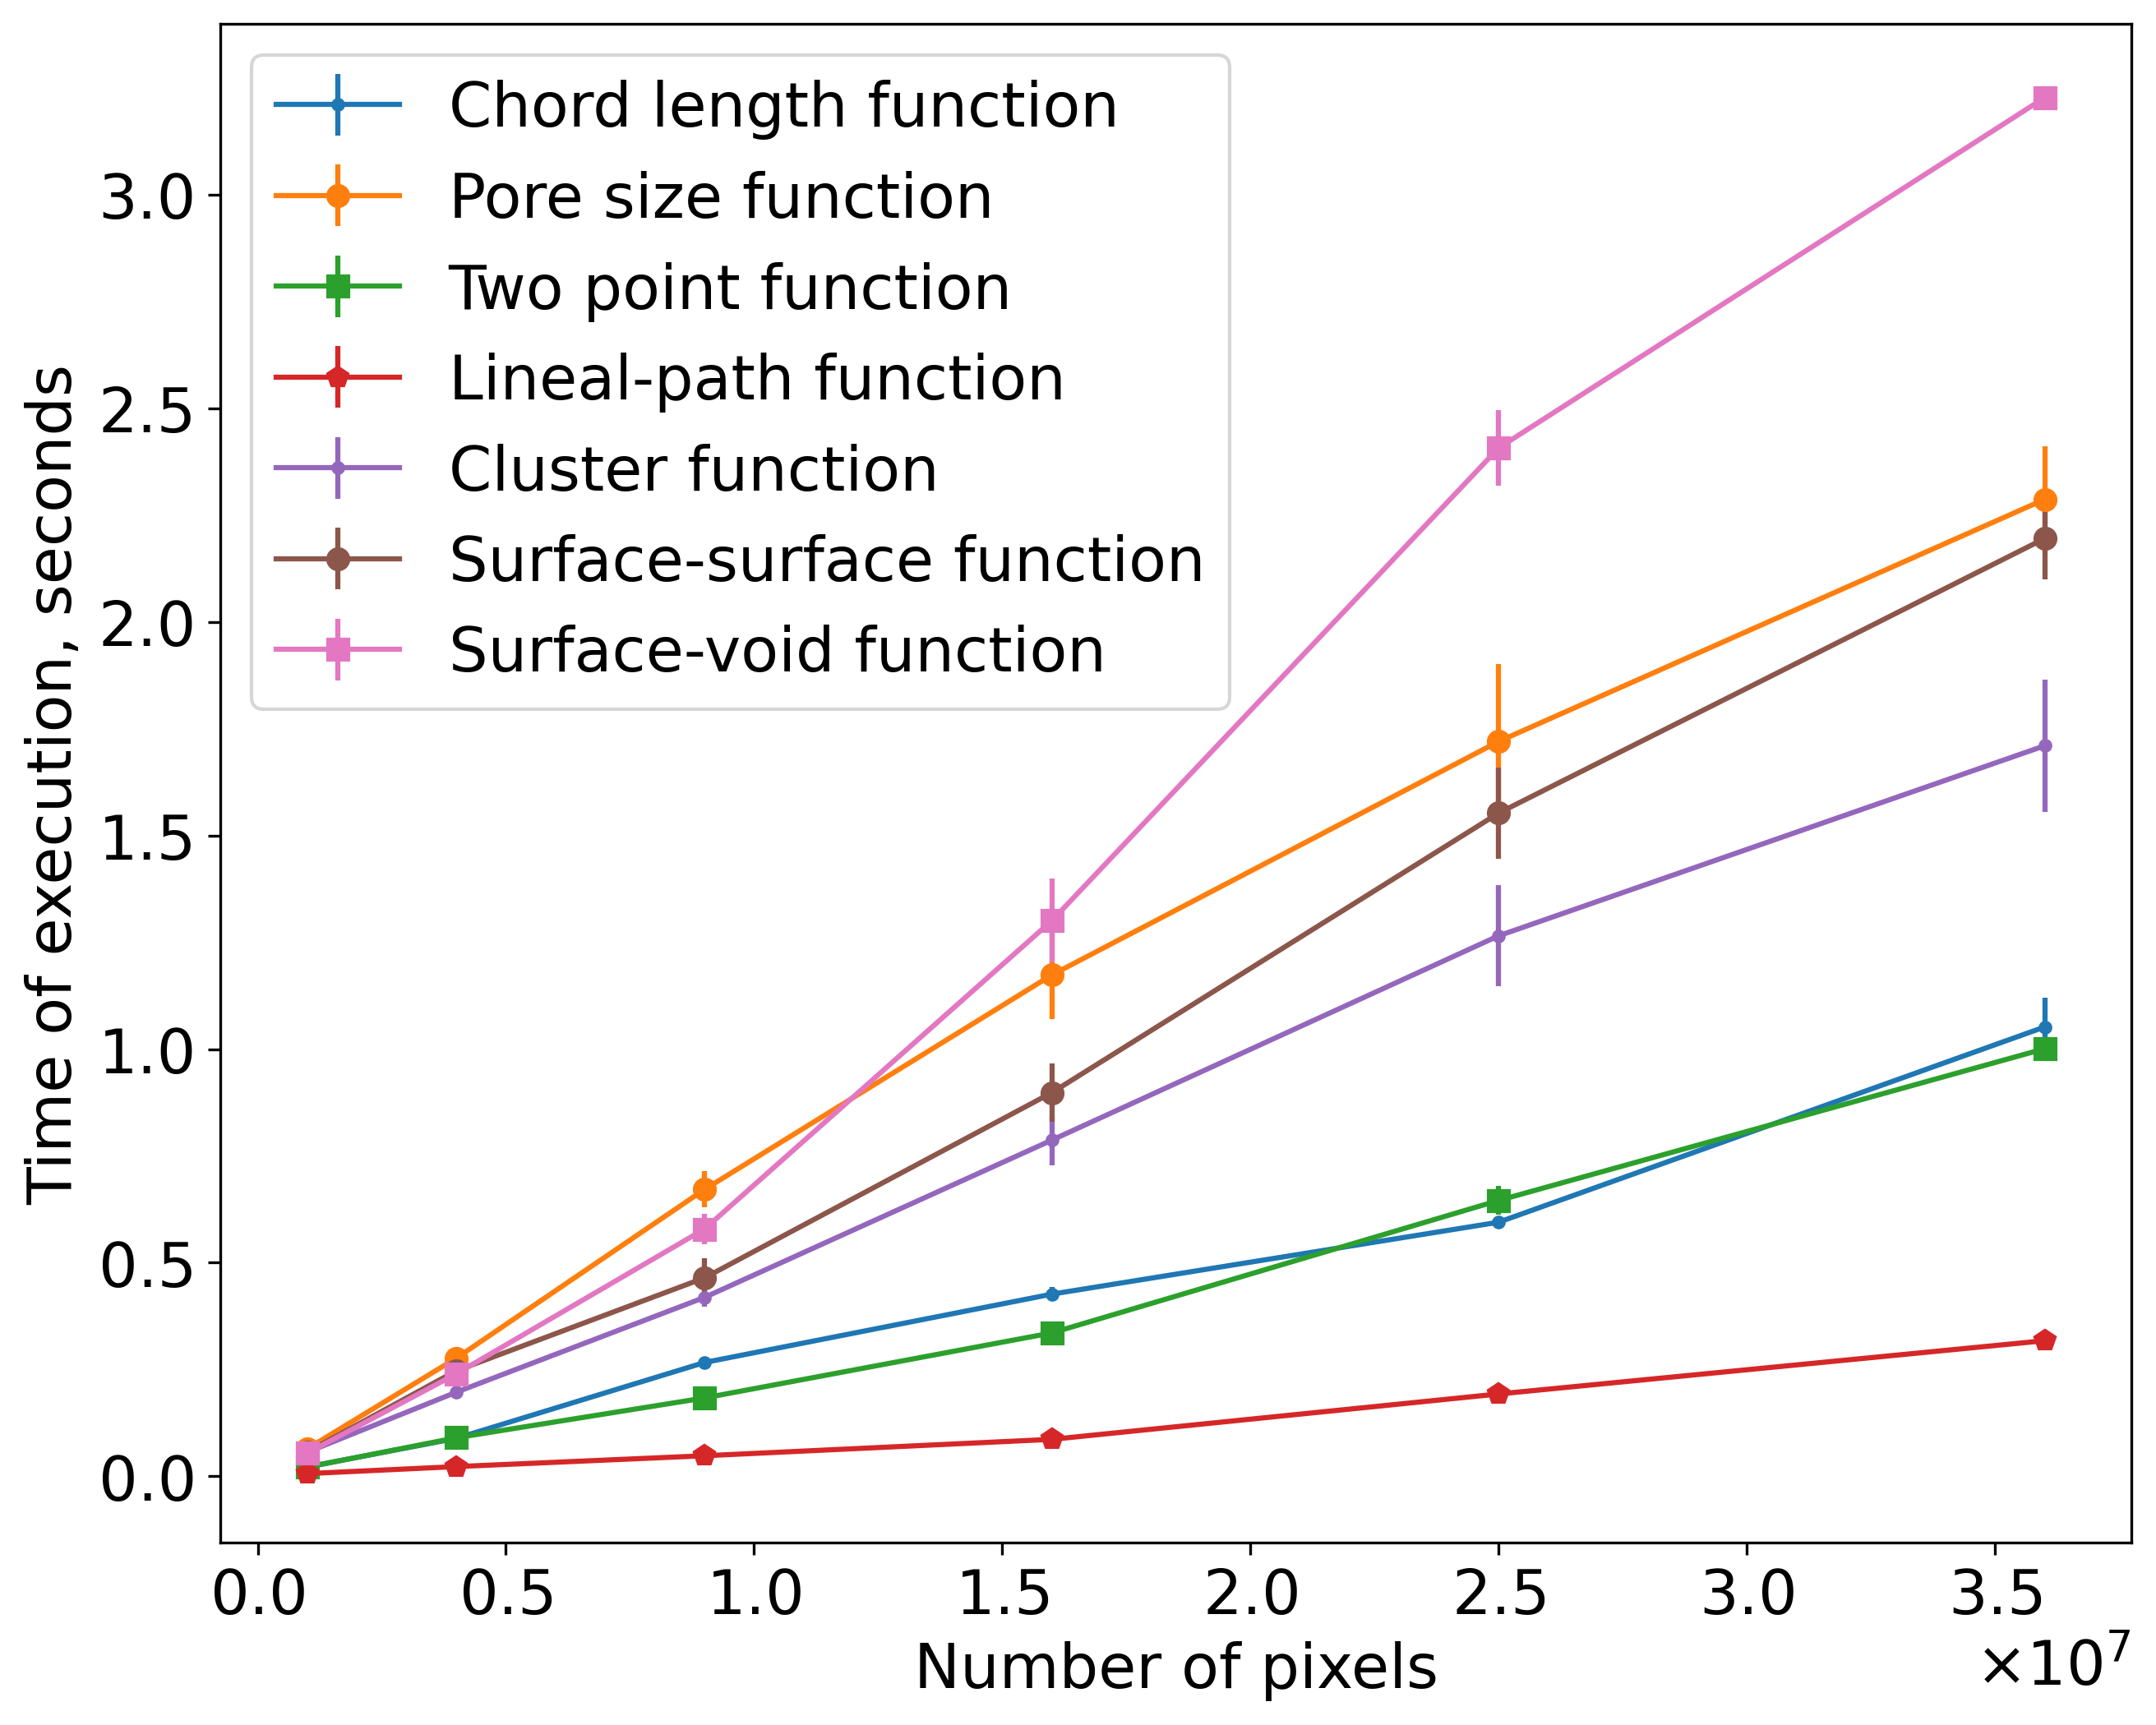
\includegraphics[width=0.475\linewidth]{images/time-2d.png}
    \label{fig:timings-2d}}
  \hfill
  \subfigure[Three-dimensional case, module \code{Directional}]{
    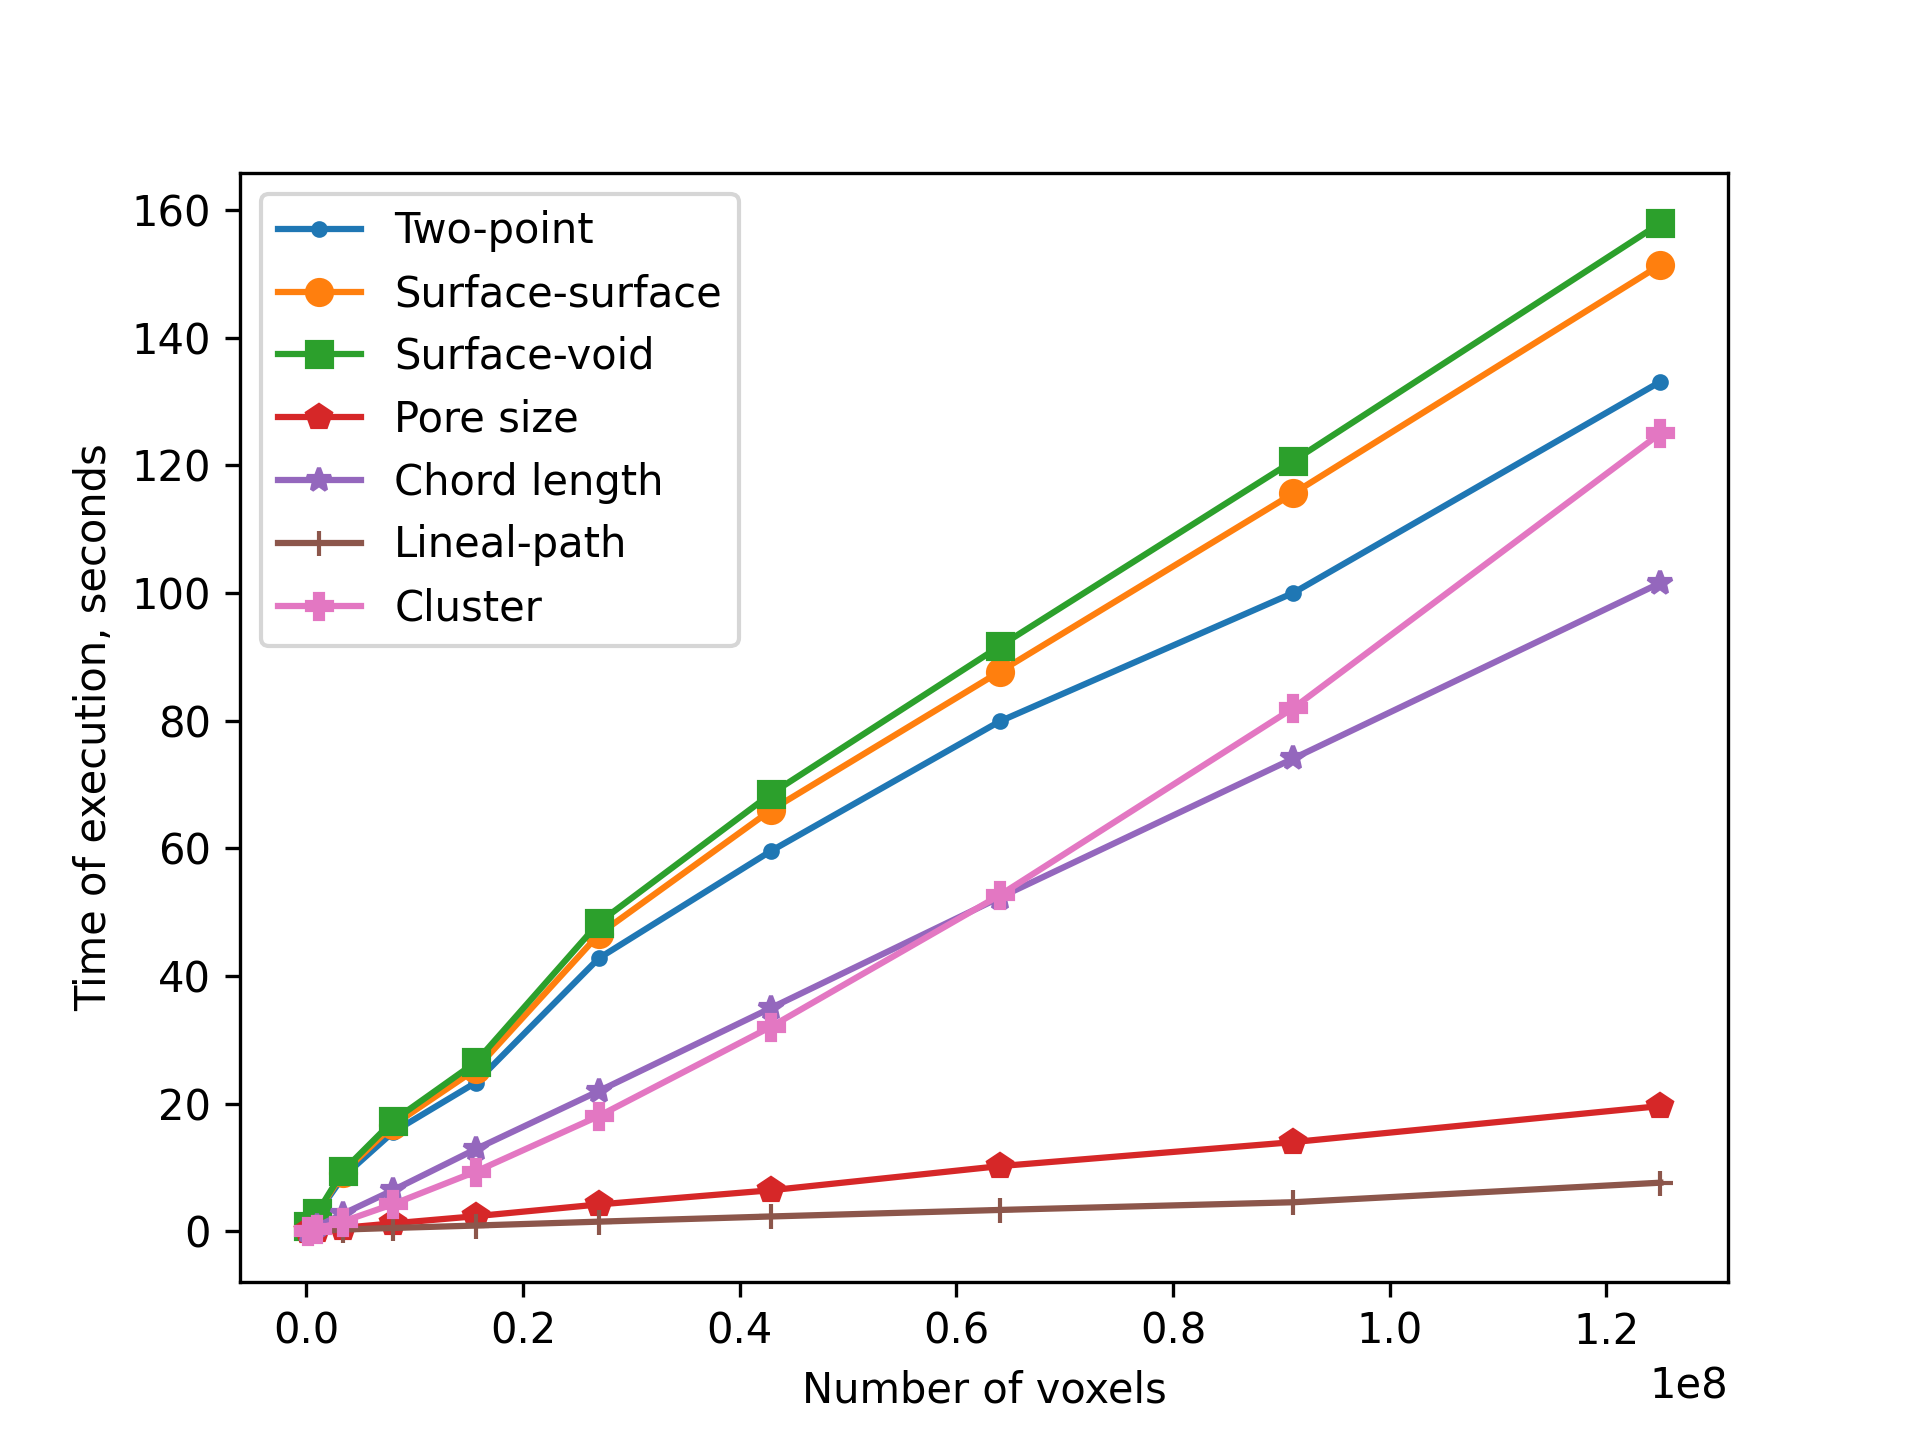
\includegraphics[width=0.475\linewidth]{images/time-3d.png}
    \label{fig:timings-3d}}
  \vskip\baselineskip
  \subfigure[Two-dimensional case, module \code{Map}, CPU]{
    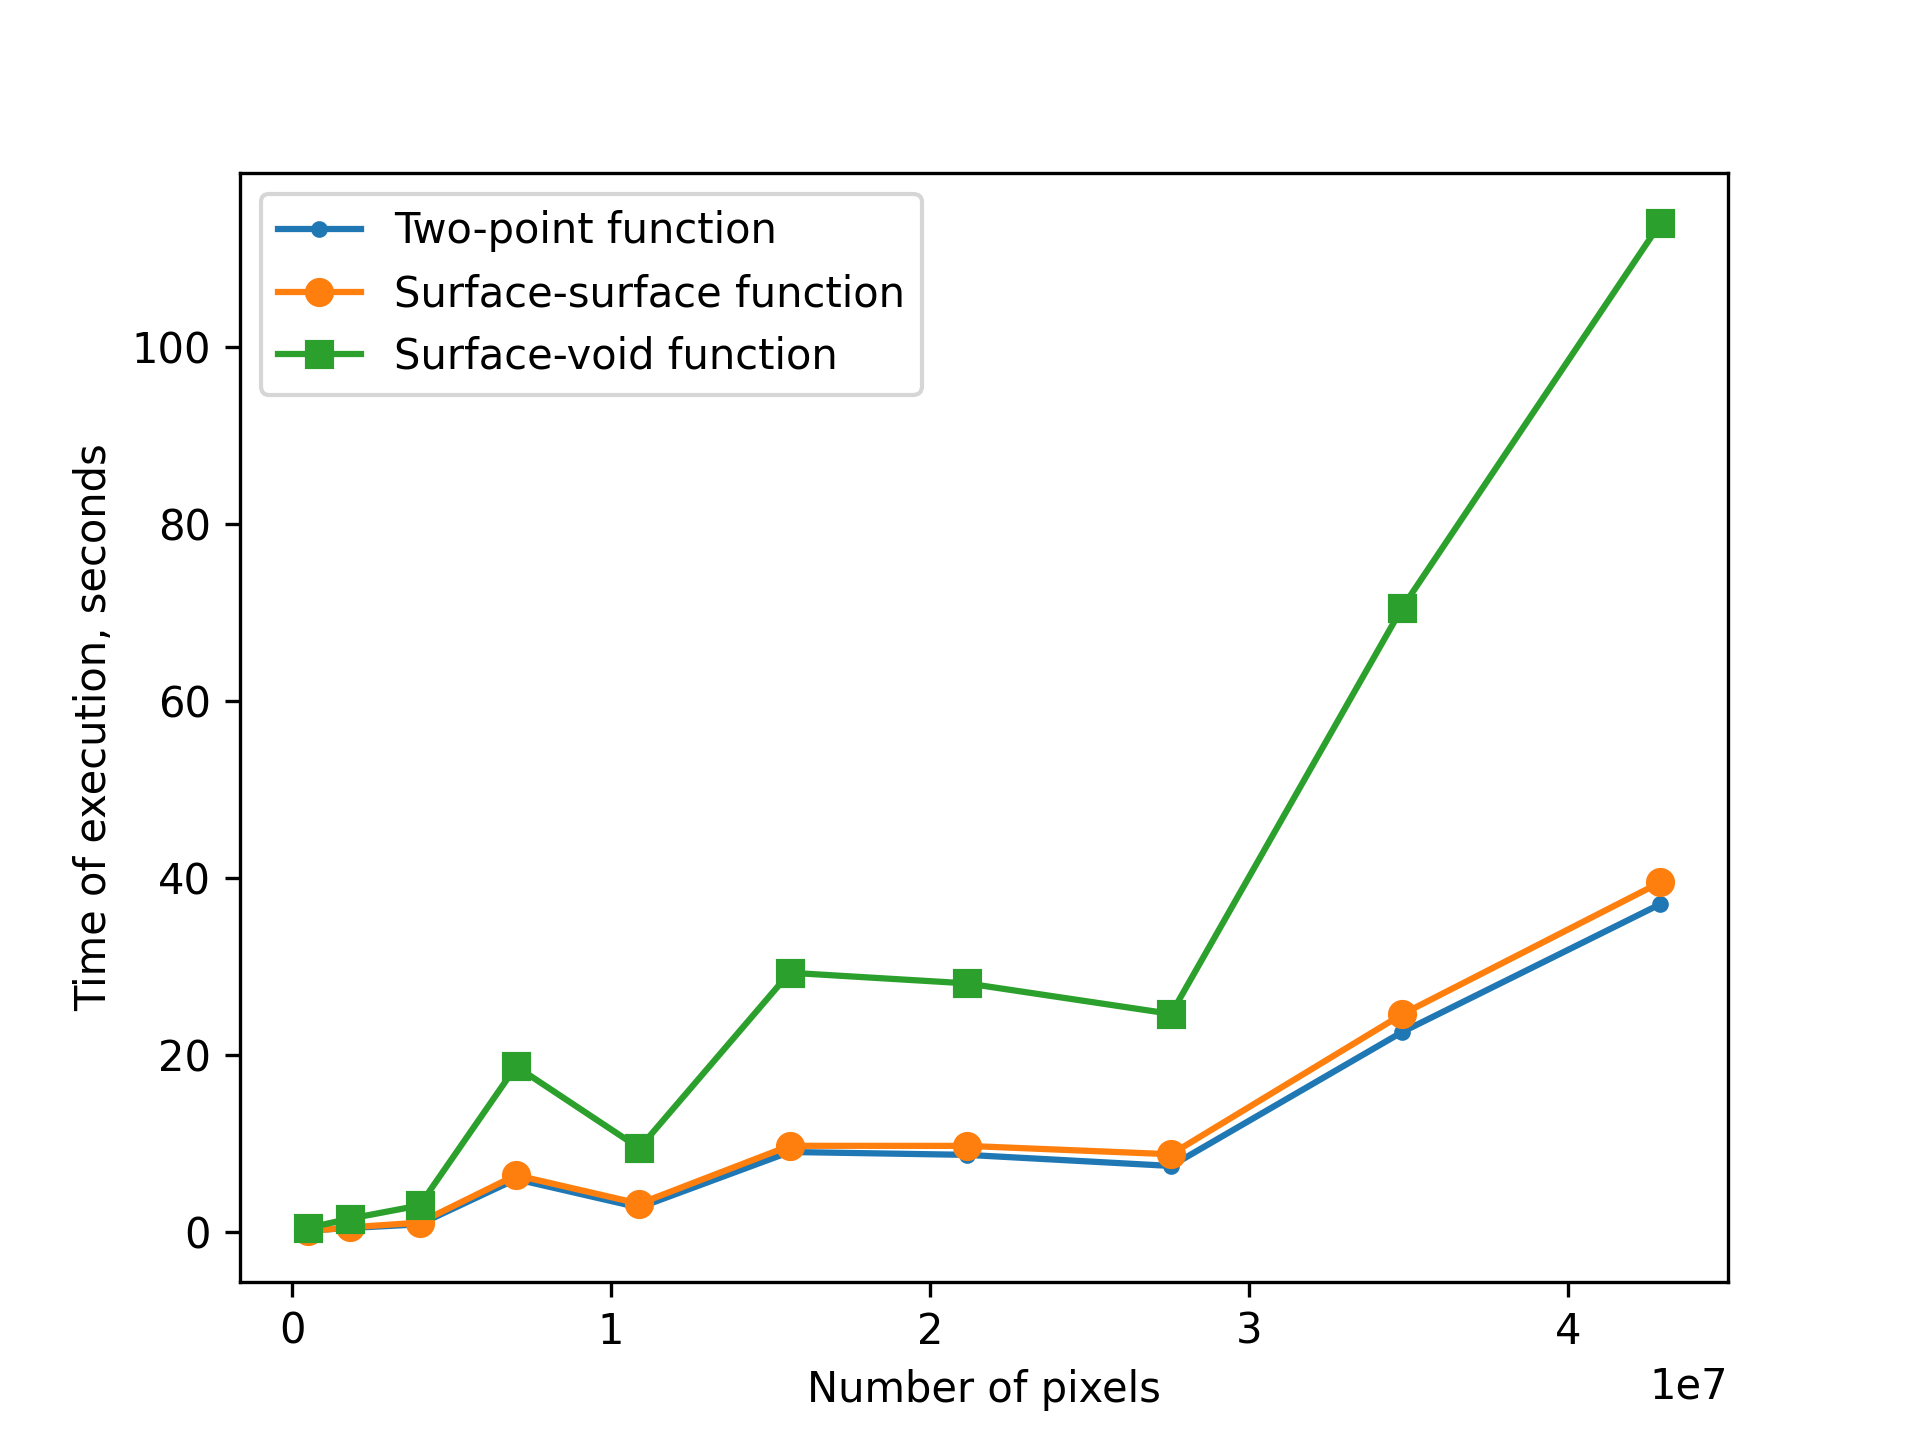
\includegraphics[width=0.475\linewidth]{images/time-2d-map.png}
    \label{fig:timings-2d-map}}
  \hfill
  \subfigure[Three-dimensional case, module \code{Map}, CPU]{
    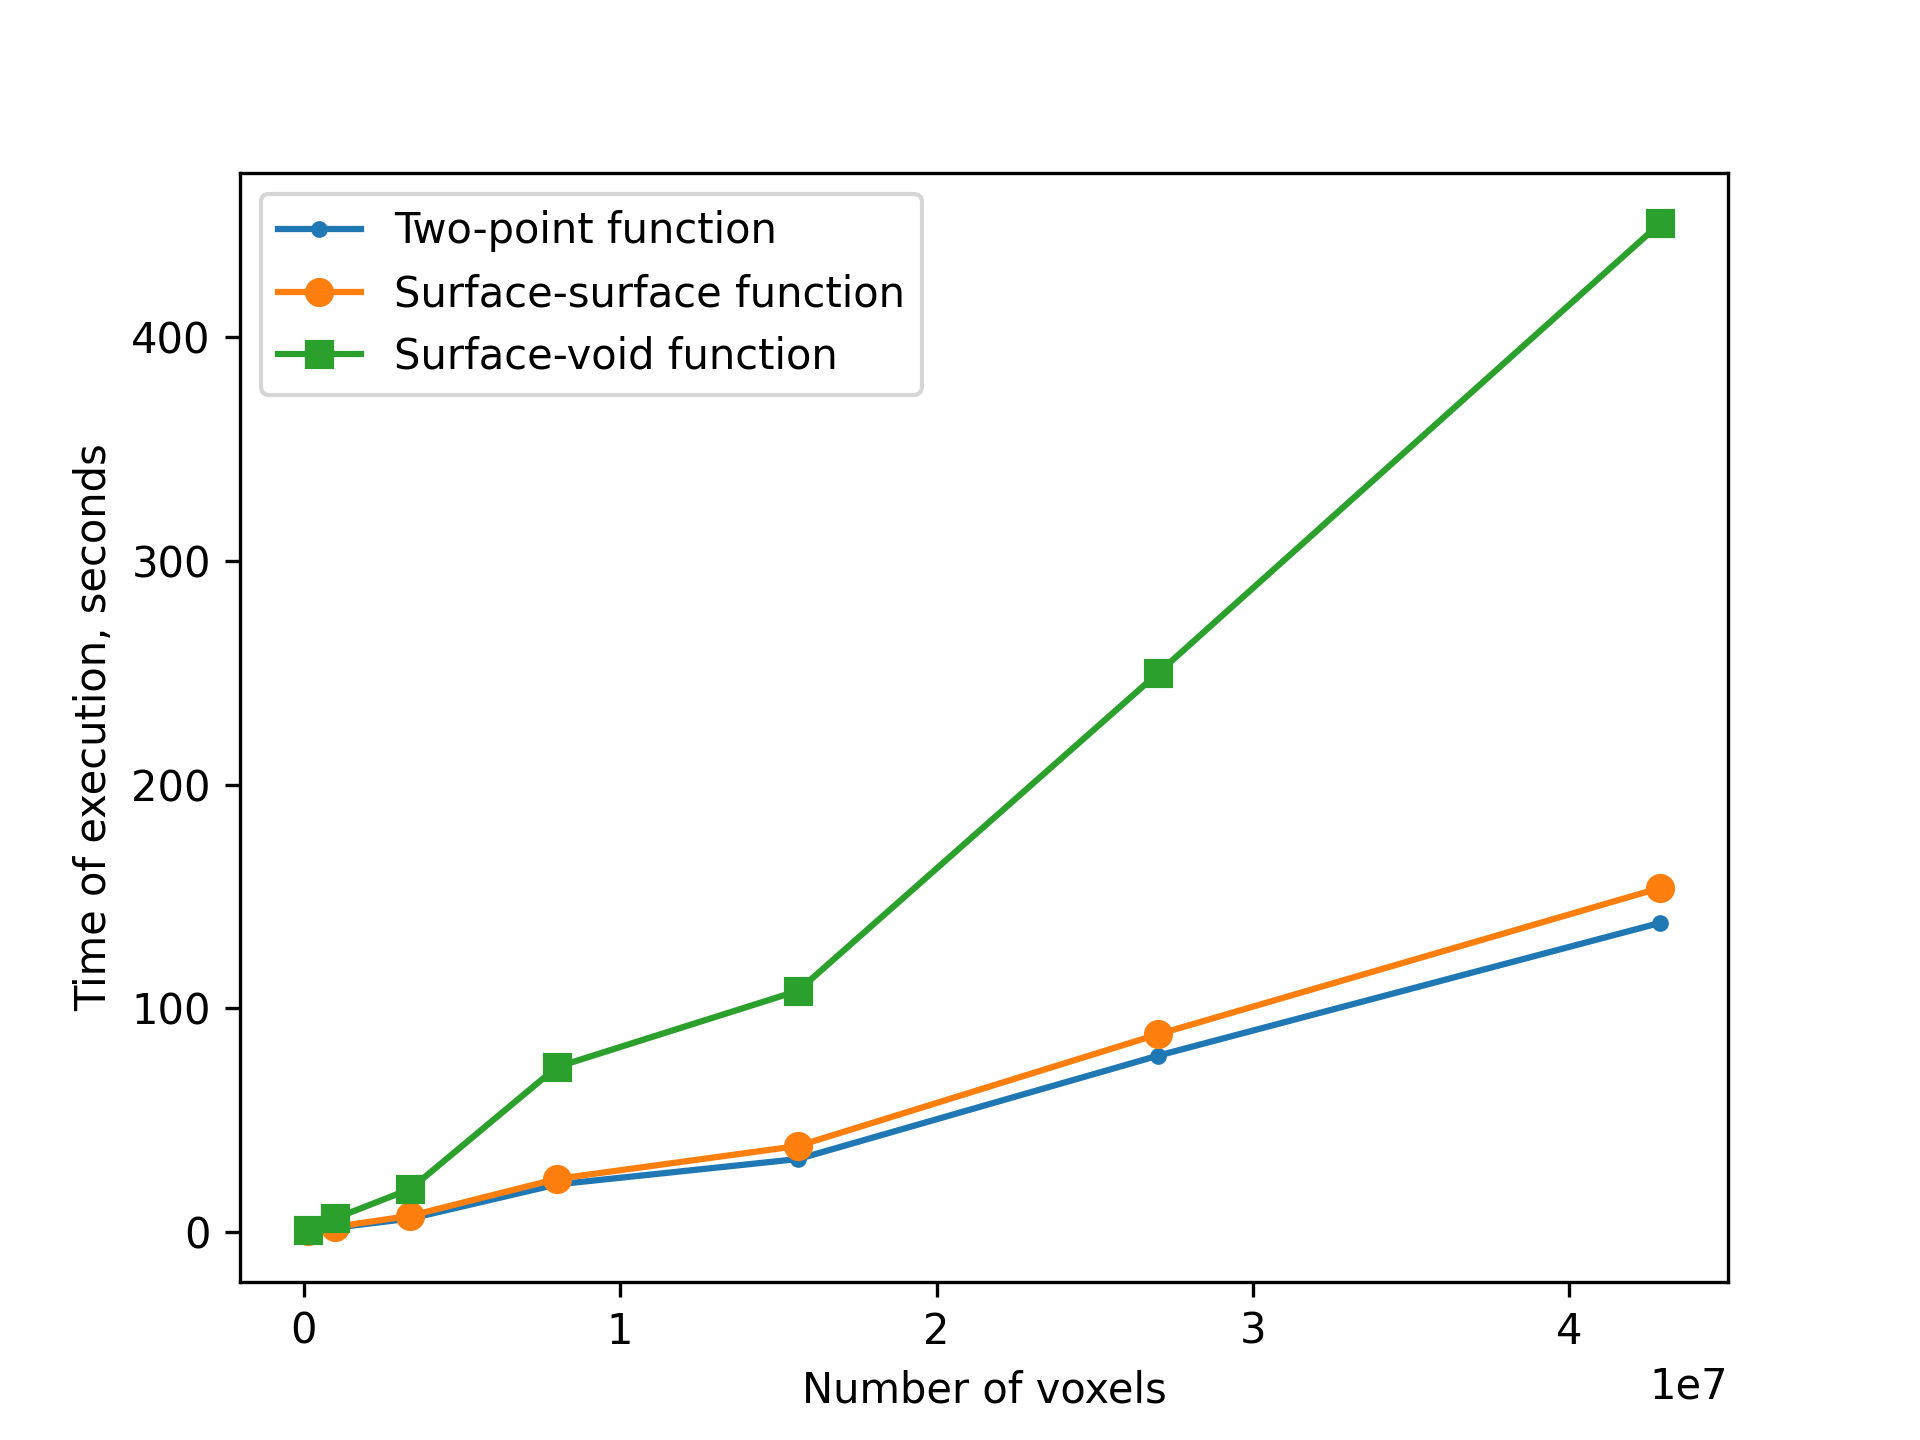
\includegraphics[width=0.475\linewidth]{images/time-3d-map.png}
    \label{fig:timings-3d-map}}
  \vskip\baselineskip
  \subfigure[Two-dimensional case, module \code{Map}, GPU]{
    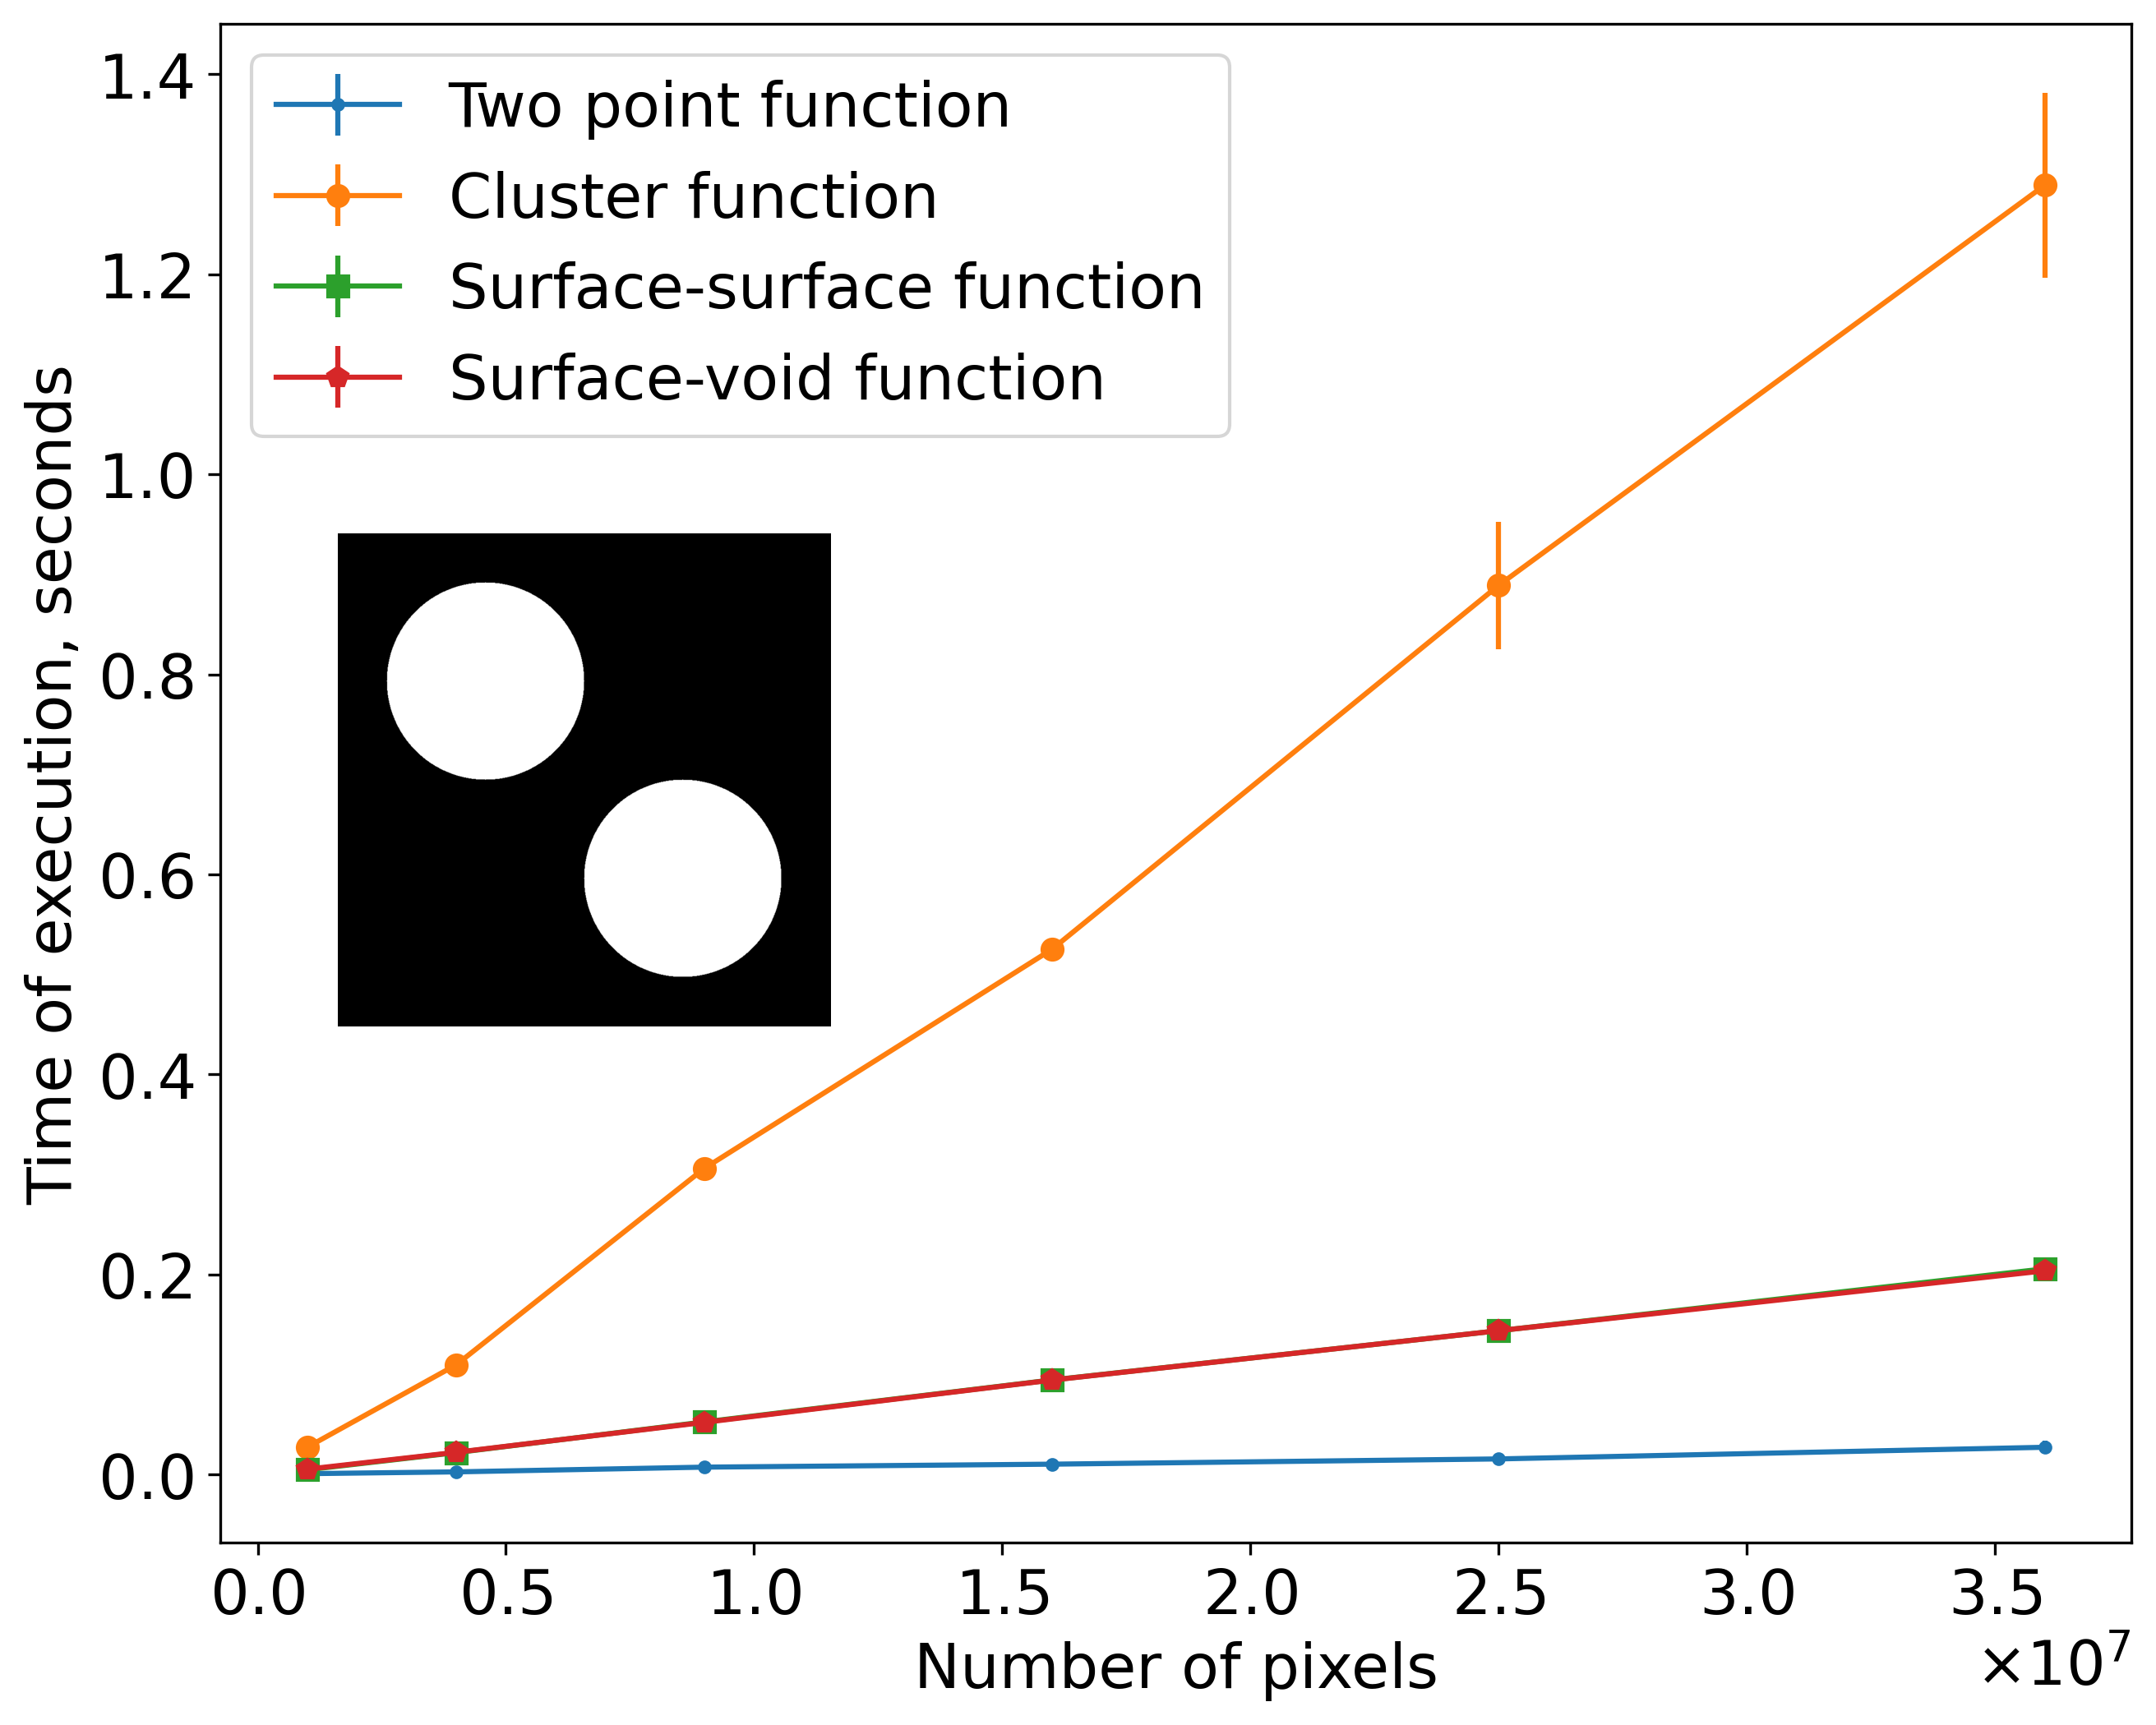
\includegraphics[width=0.475\linewidth]{images/time-2d-gpu.png}
    \label{fig:timings-2d-gpu}}
  \hfill
  \subfigure[Three-dimensional case, module \code{Map}, GPU]{
    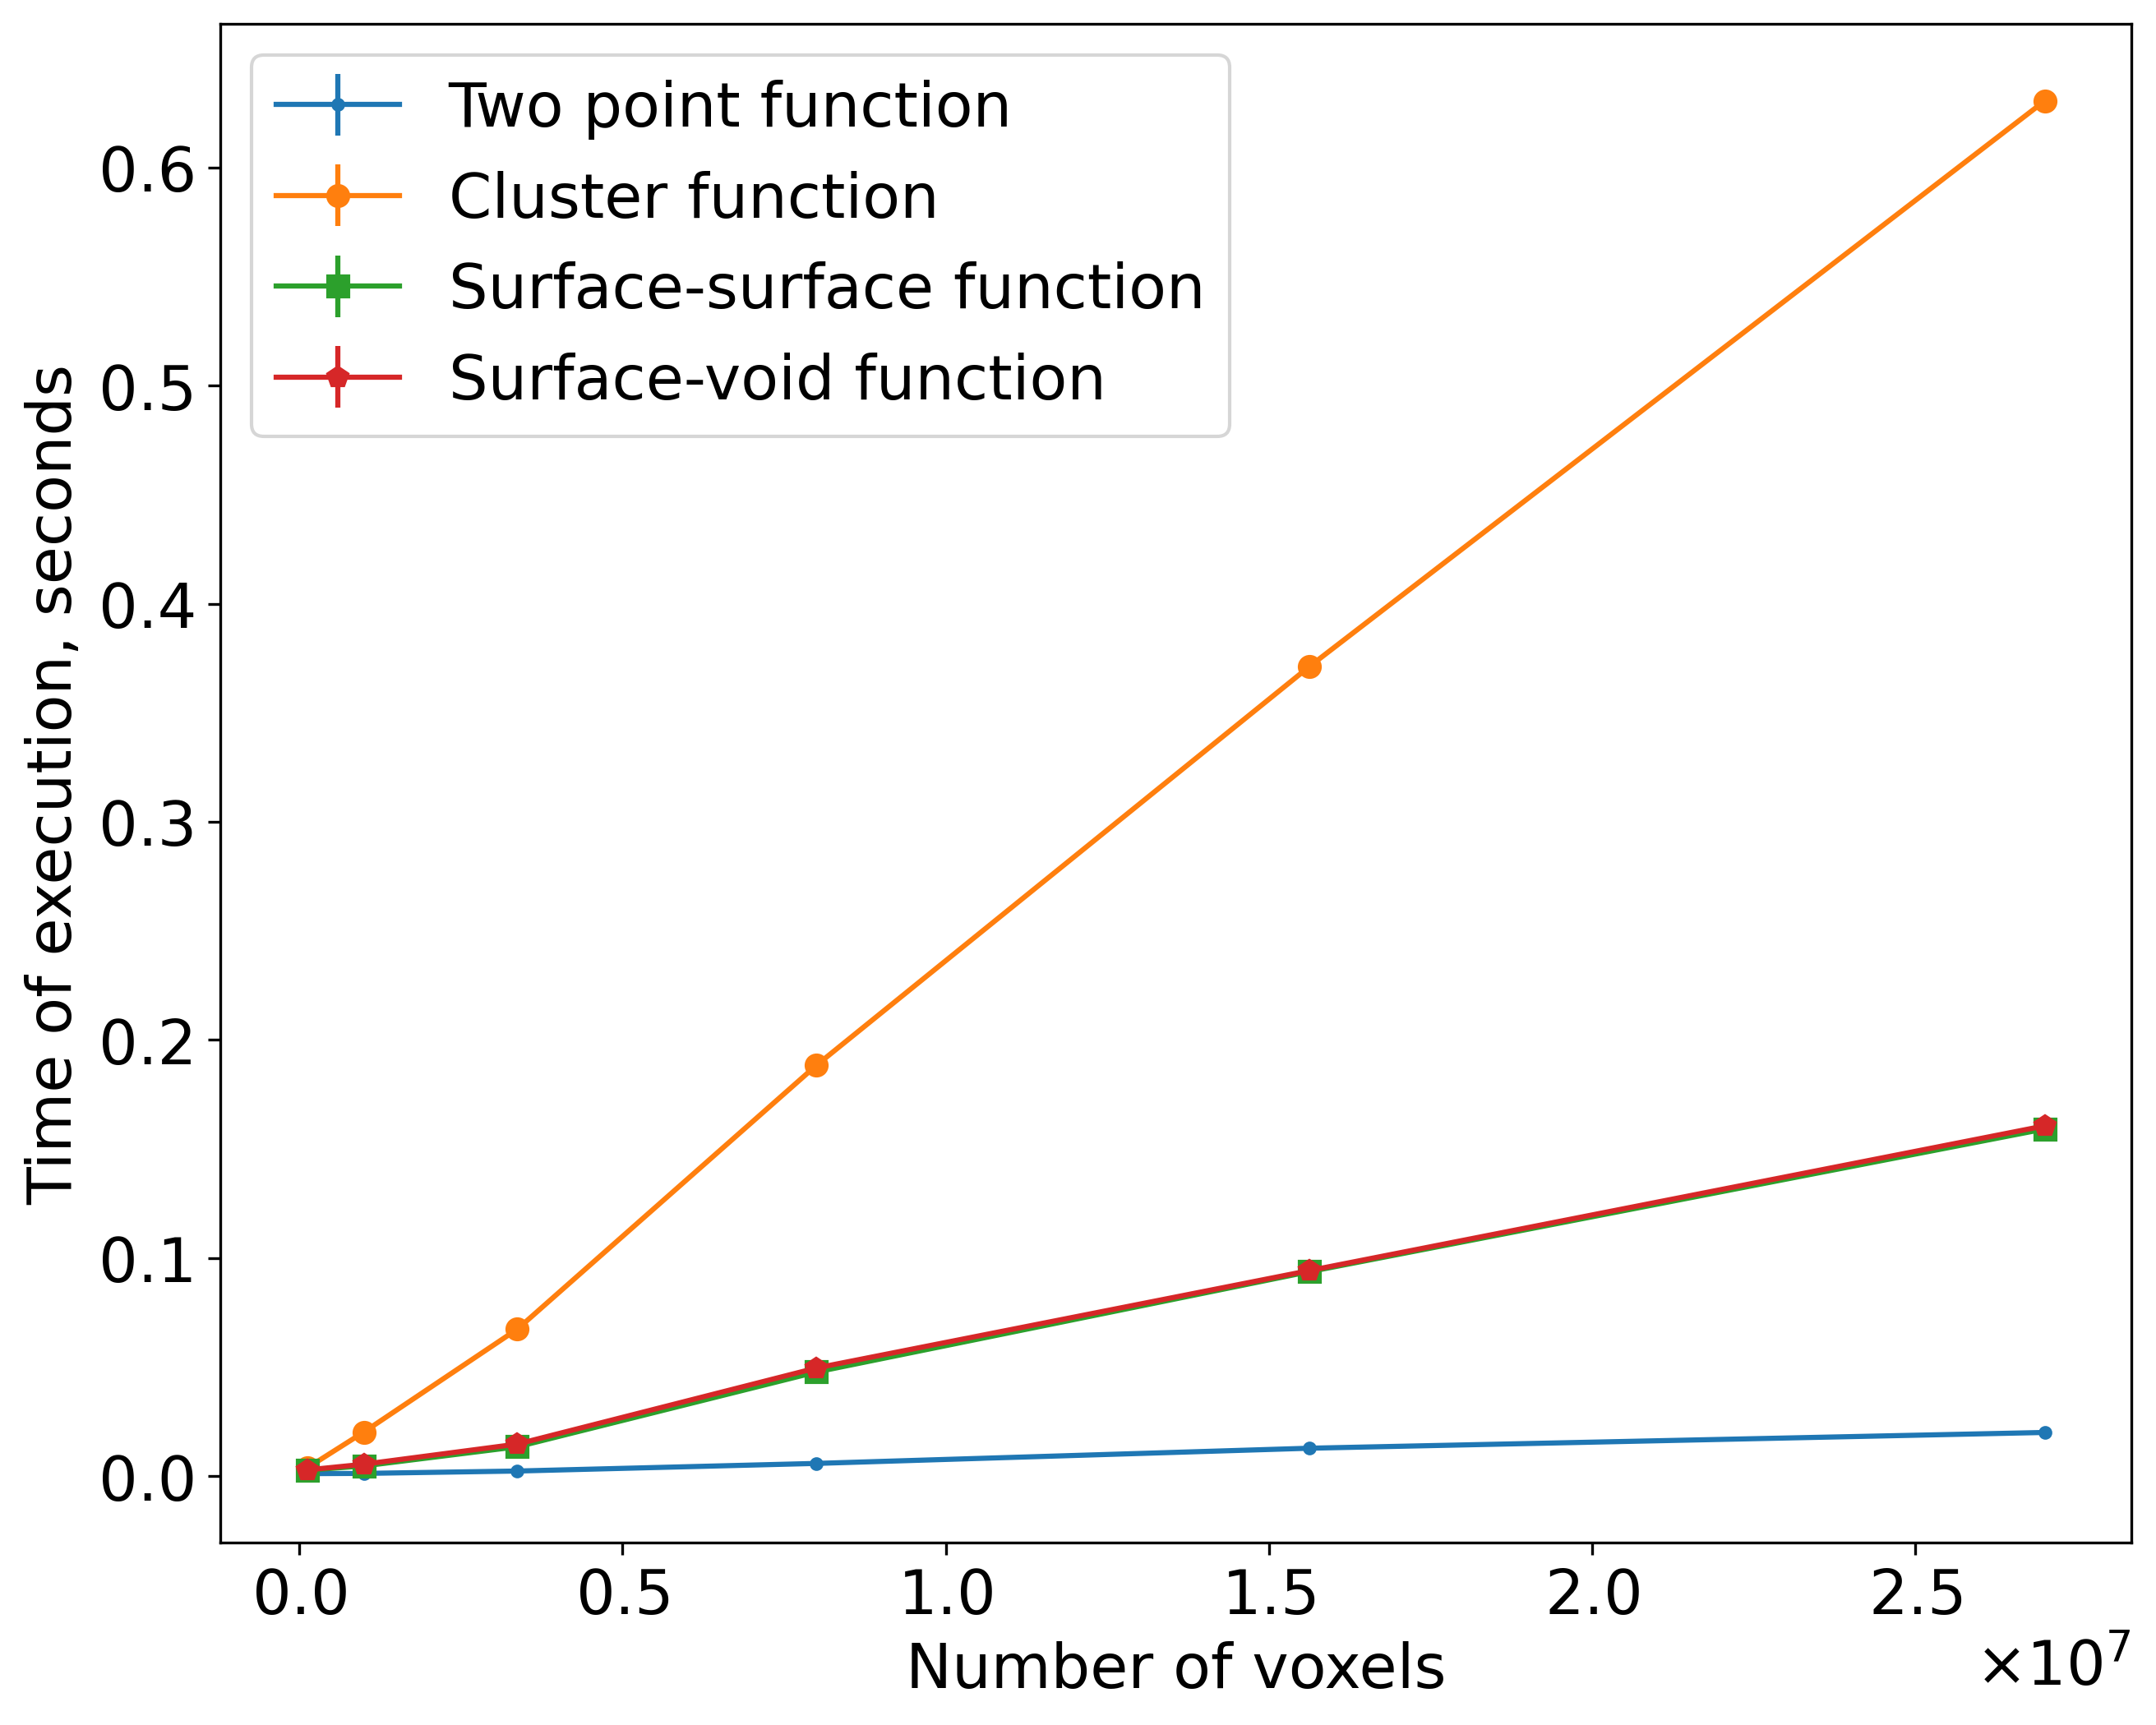
\includegraphics[width=0.475\linewidth]{images/time-3d-gpu.png}
    \label{fig:timings-3d-gpu}}
  \caption[]{Execution times for different correlation functions.}
  \label{fig:timings}
\end{figure*}

\section{Examples and applications}
\label{sec:examples}
After the verification of our computational approach based on analytical
solution we can apply our algorithms to evaluate correlation functions for
different porous media images, including real XCT and SEM images.

For demonstration purposes, we computed correlation functions for images of
sandstone found on Digital Rocks Portal \cite{DigitalRocks} all of which have
dimensions $1000 \times 1000 \times 1000$. The result can be seen on
\cref{fig:real-data}.

\begin{figure*}[t]
  \centering
  \subfigure[$S_2^{(void)}$ correlation function.]{
    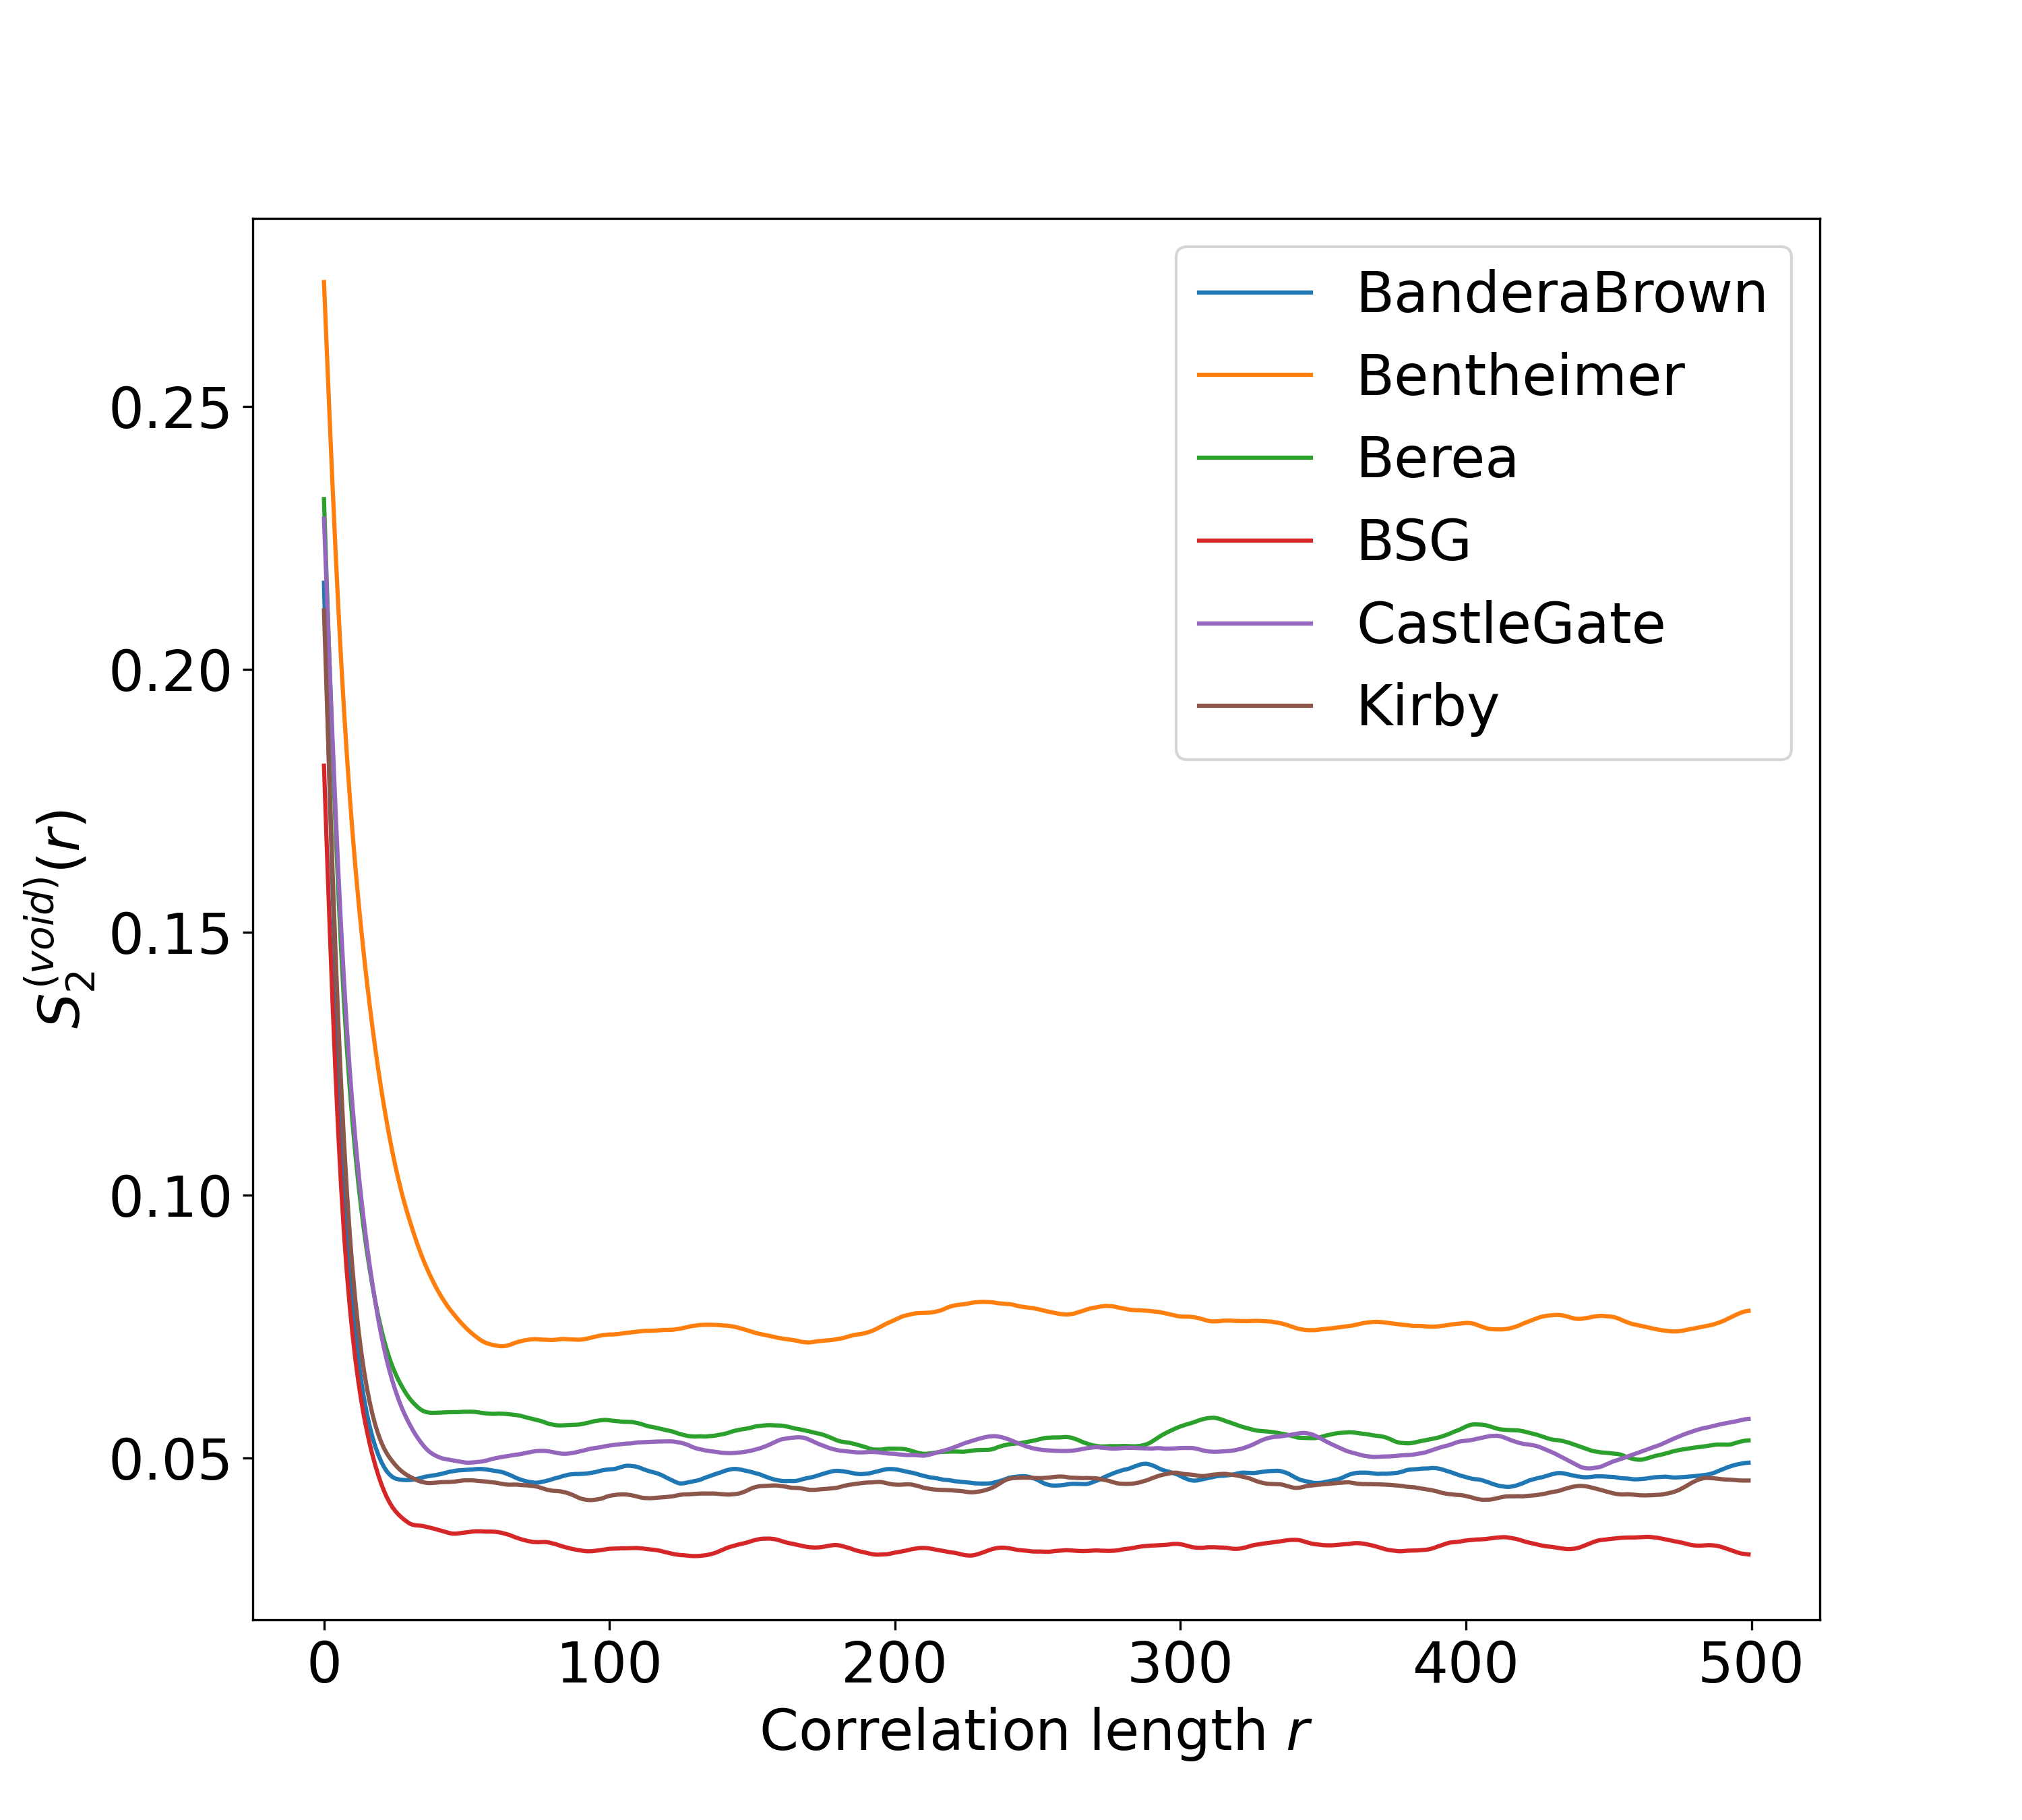
\includegraphics[width=0.3\linewidth]{real-data-plots/real-s2void.png}
    \label{fig:real-s2}}
  \hfill
  \subfigure[$L_2^{(void)}$ correlation function.]{
    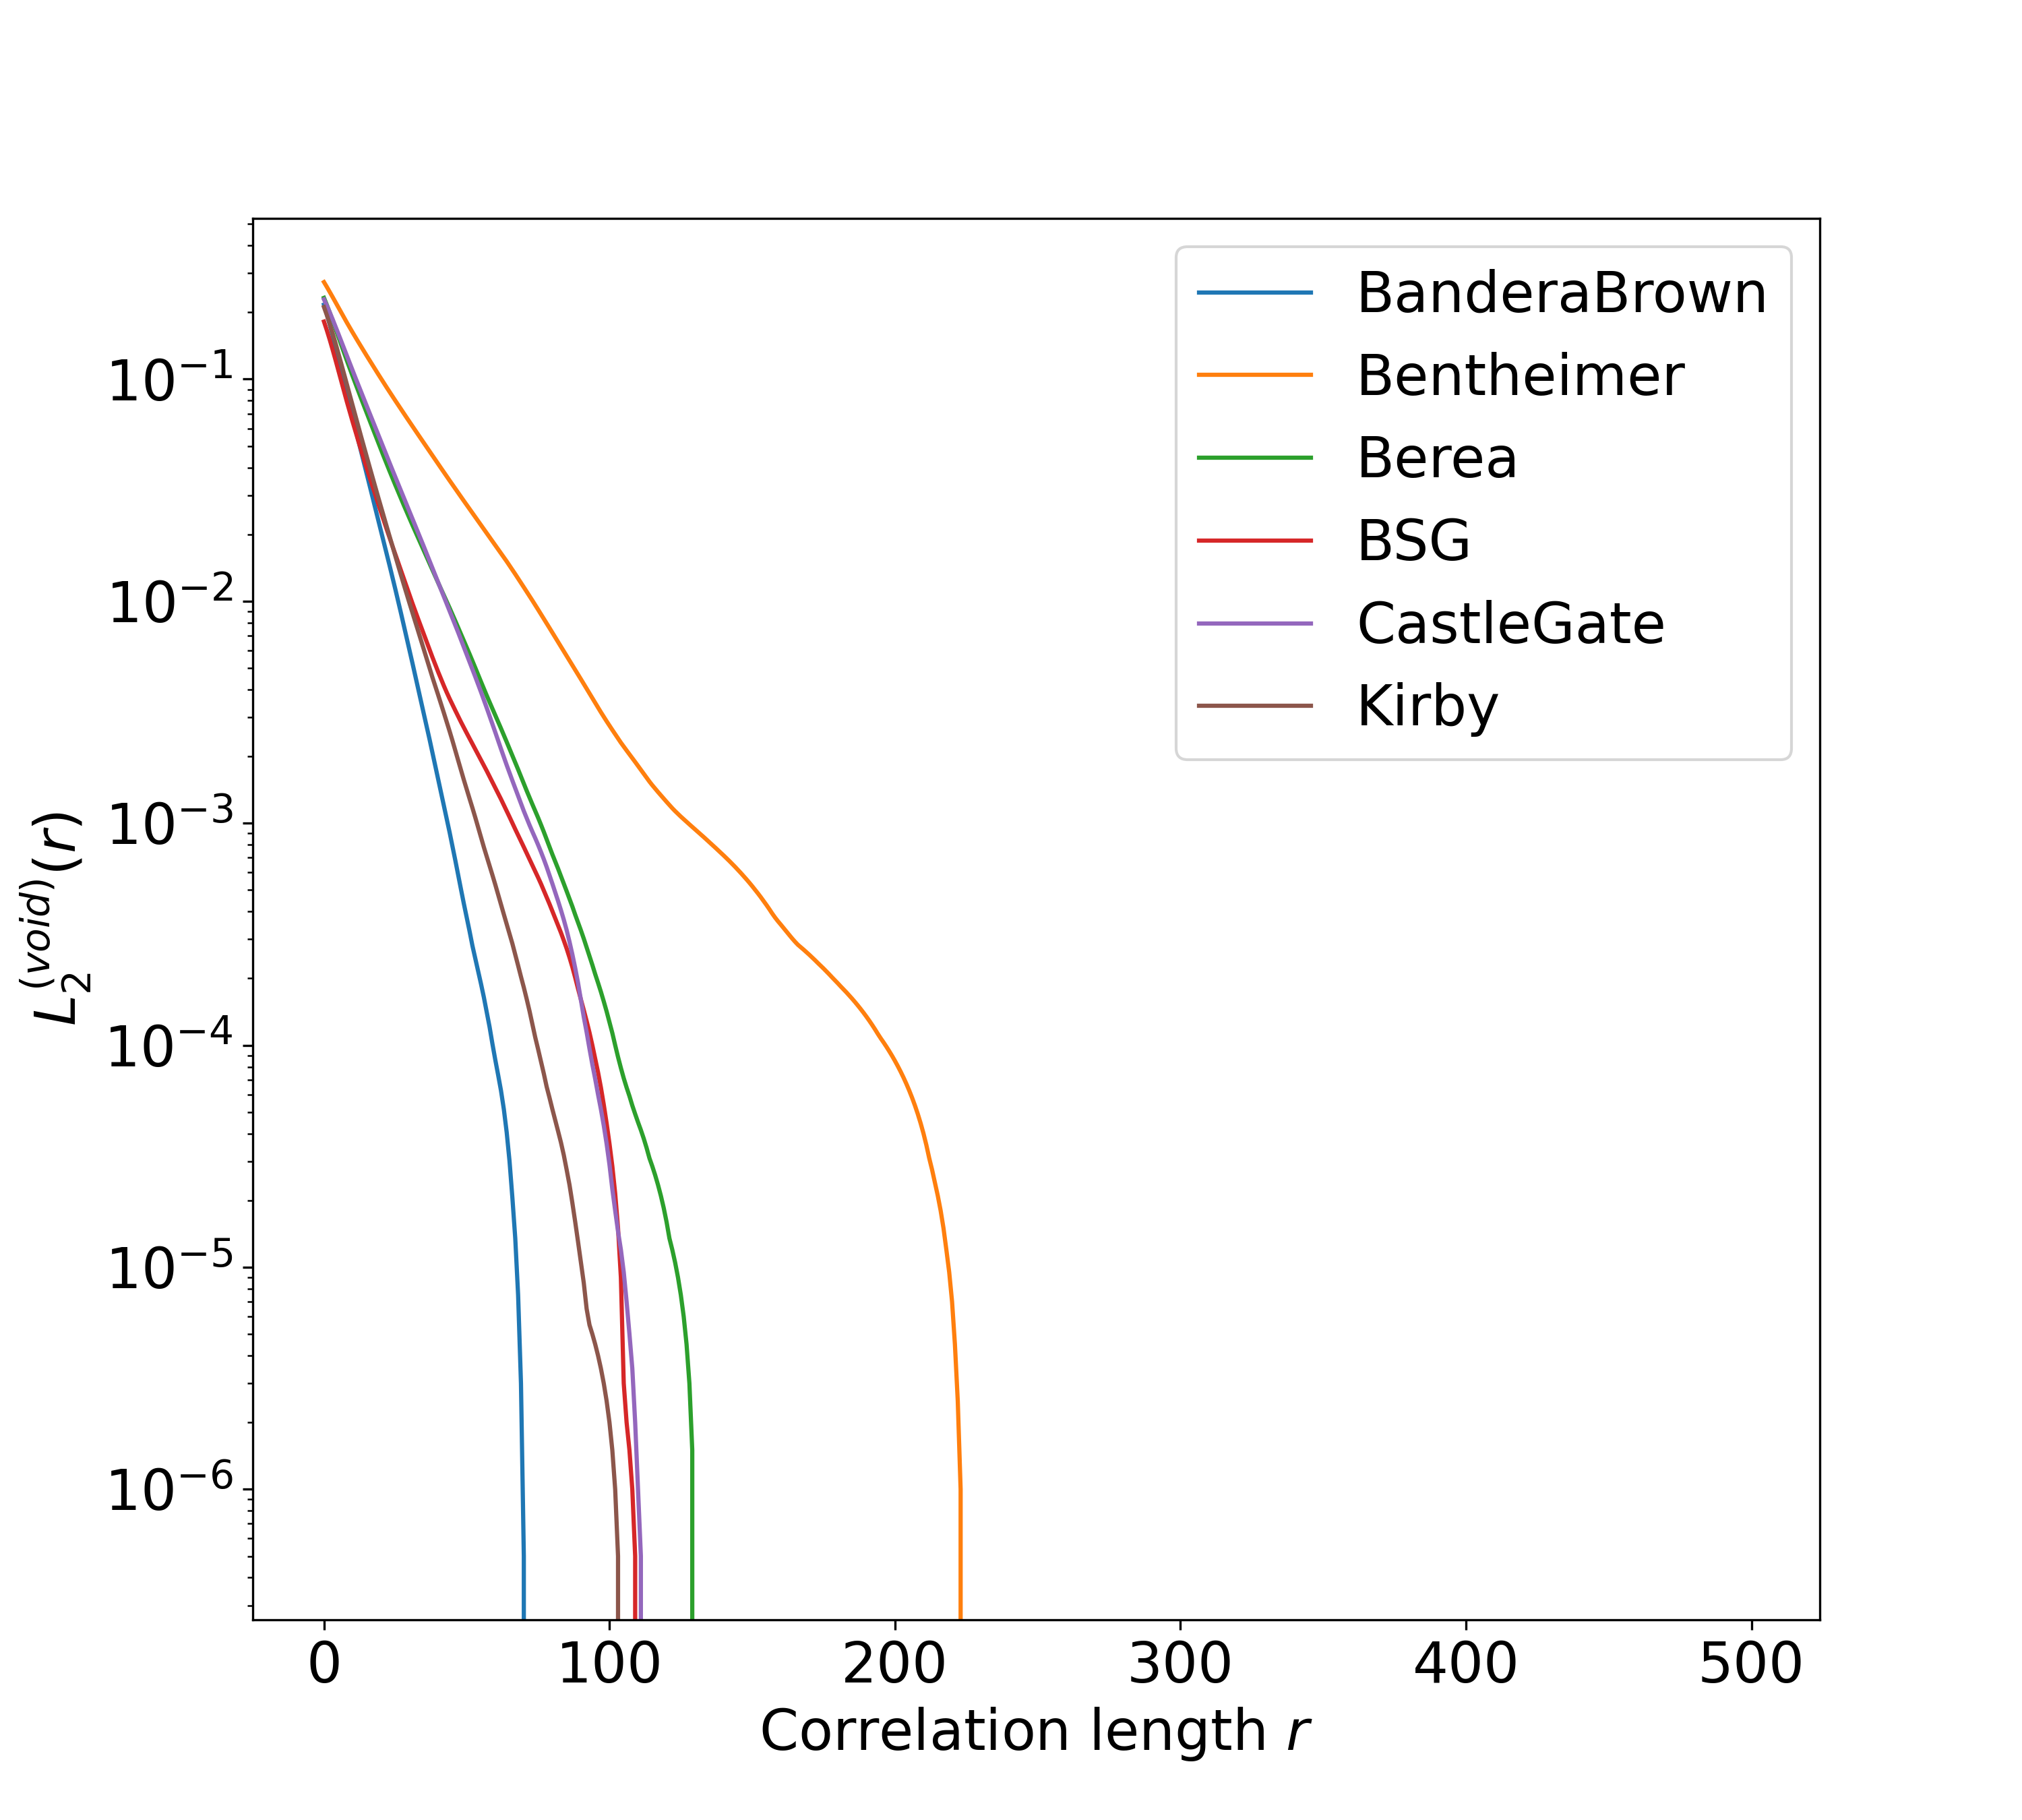
\includegraphics[width=0.3\linewidth]{real-data-plots/real-l2void.png}
    \label{fig:real-l2}}
  \subfigure[$C_2^{(void)}$ correlation function.]{
    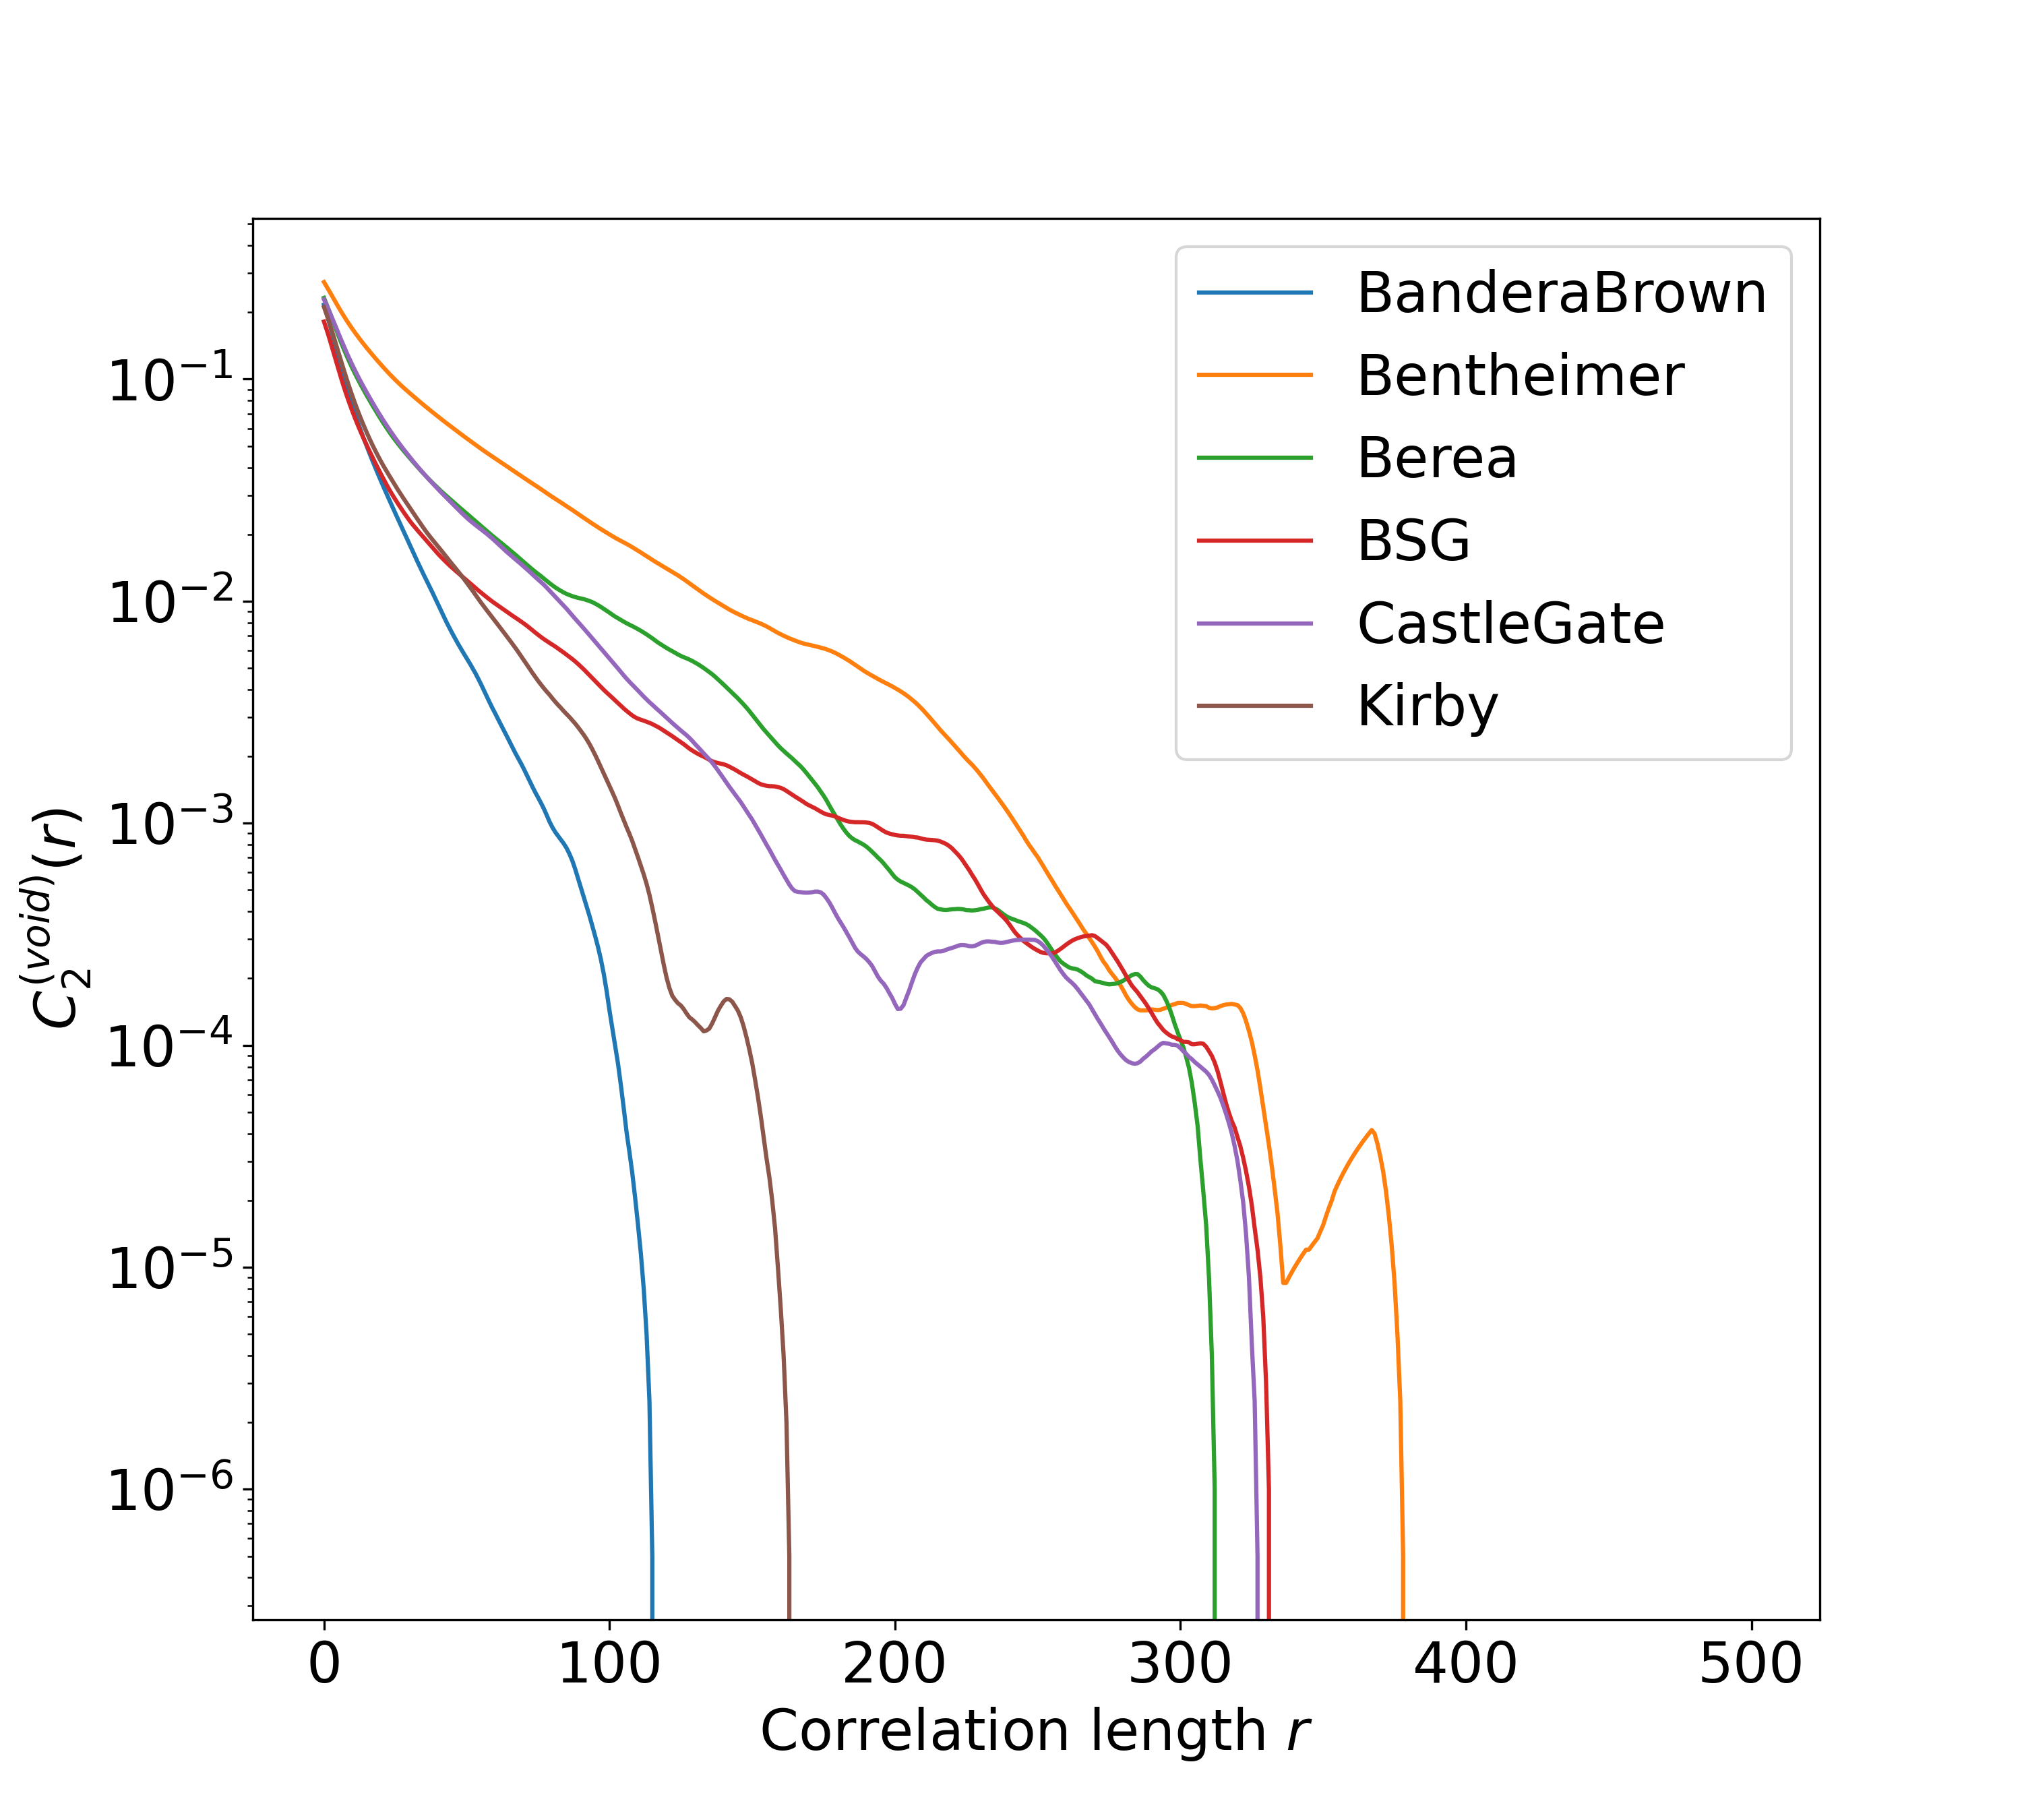
\includegraphics[width=0.3\linewidth]{real-data-plots/real-c2void.png}
    \label{fig:real-c2}}
  \vskip\baselineskip
  \subfigure[$F_{ss}$ correlation function.]{
    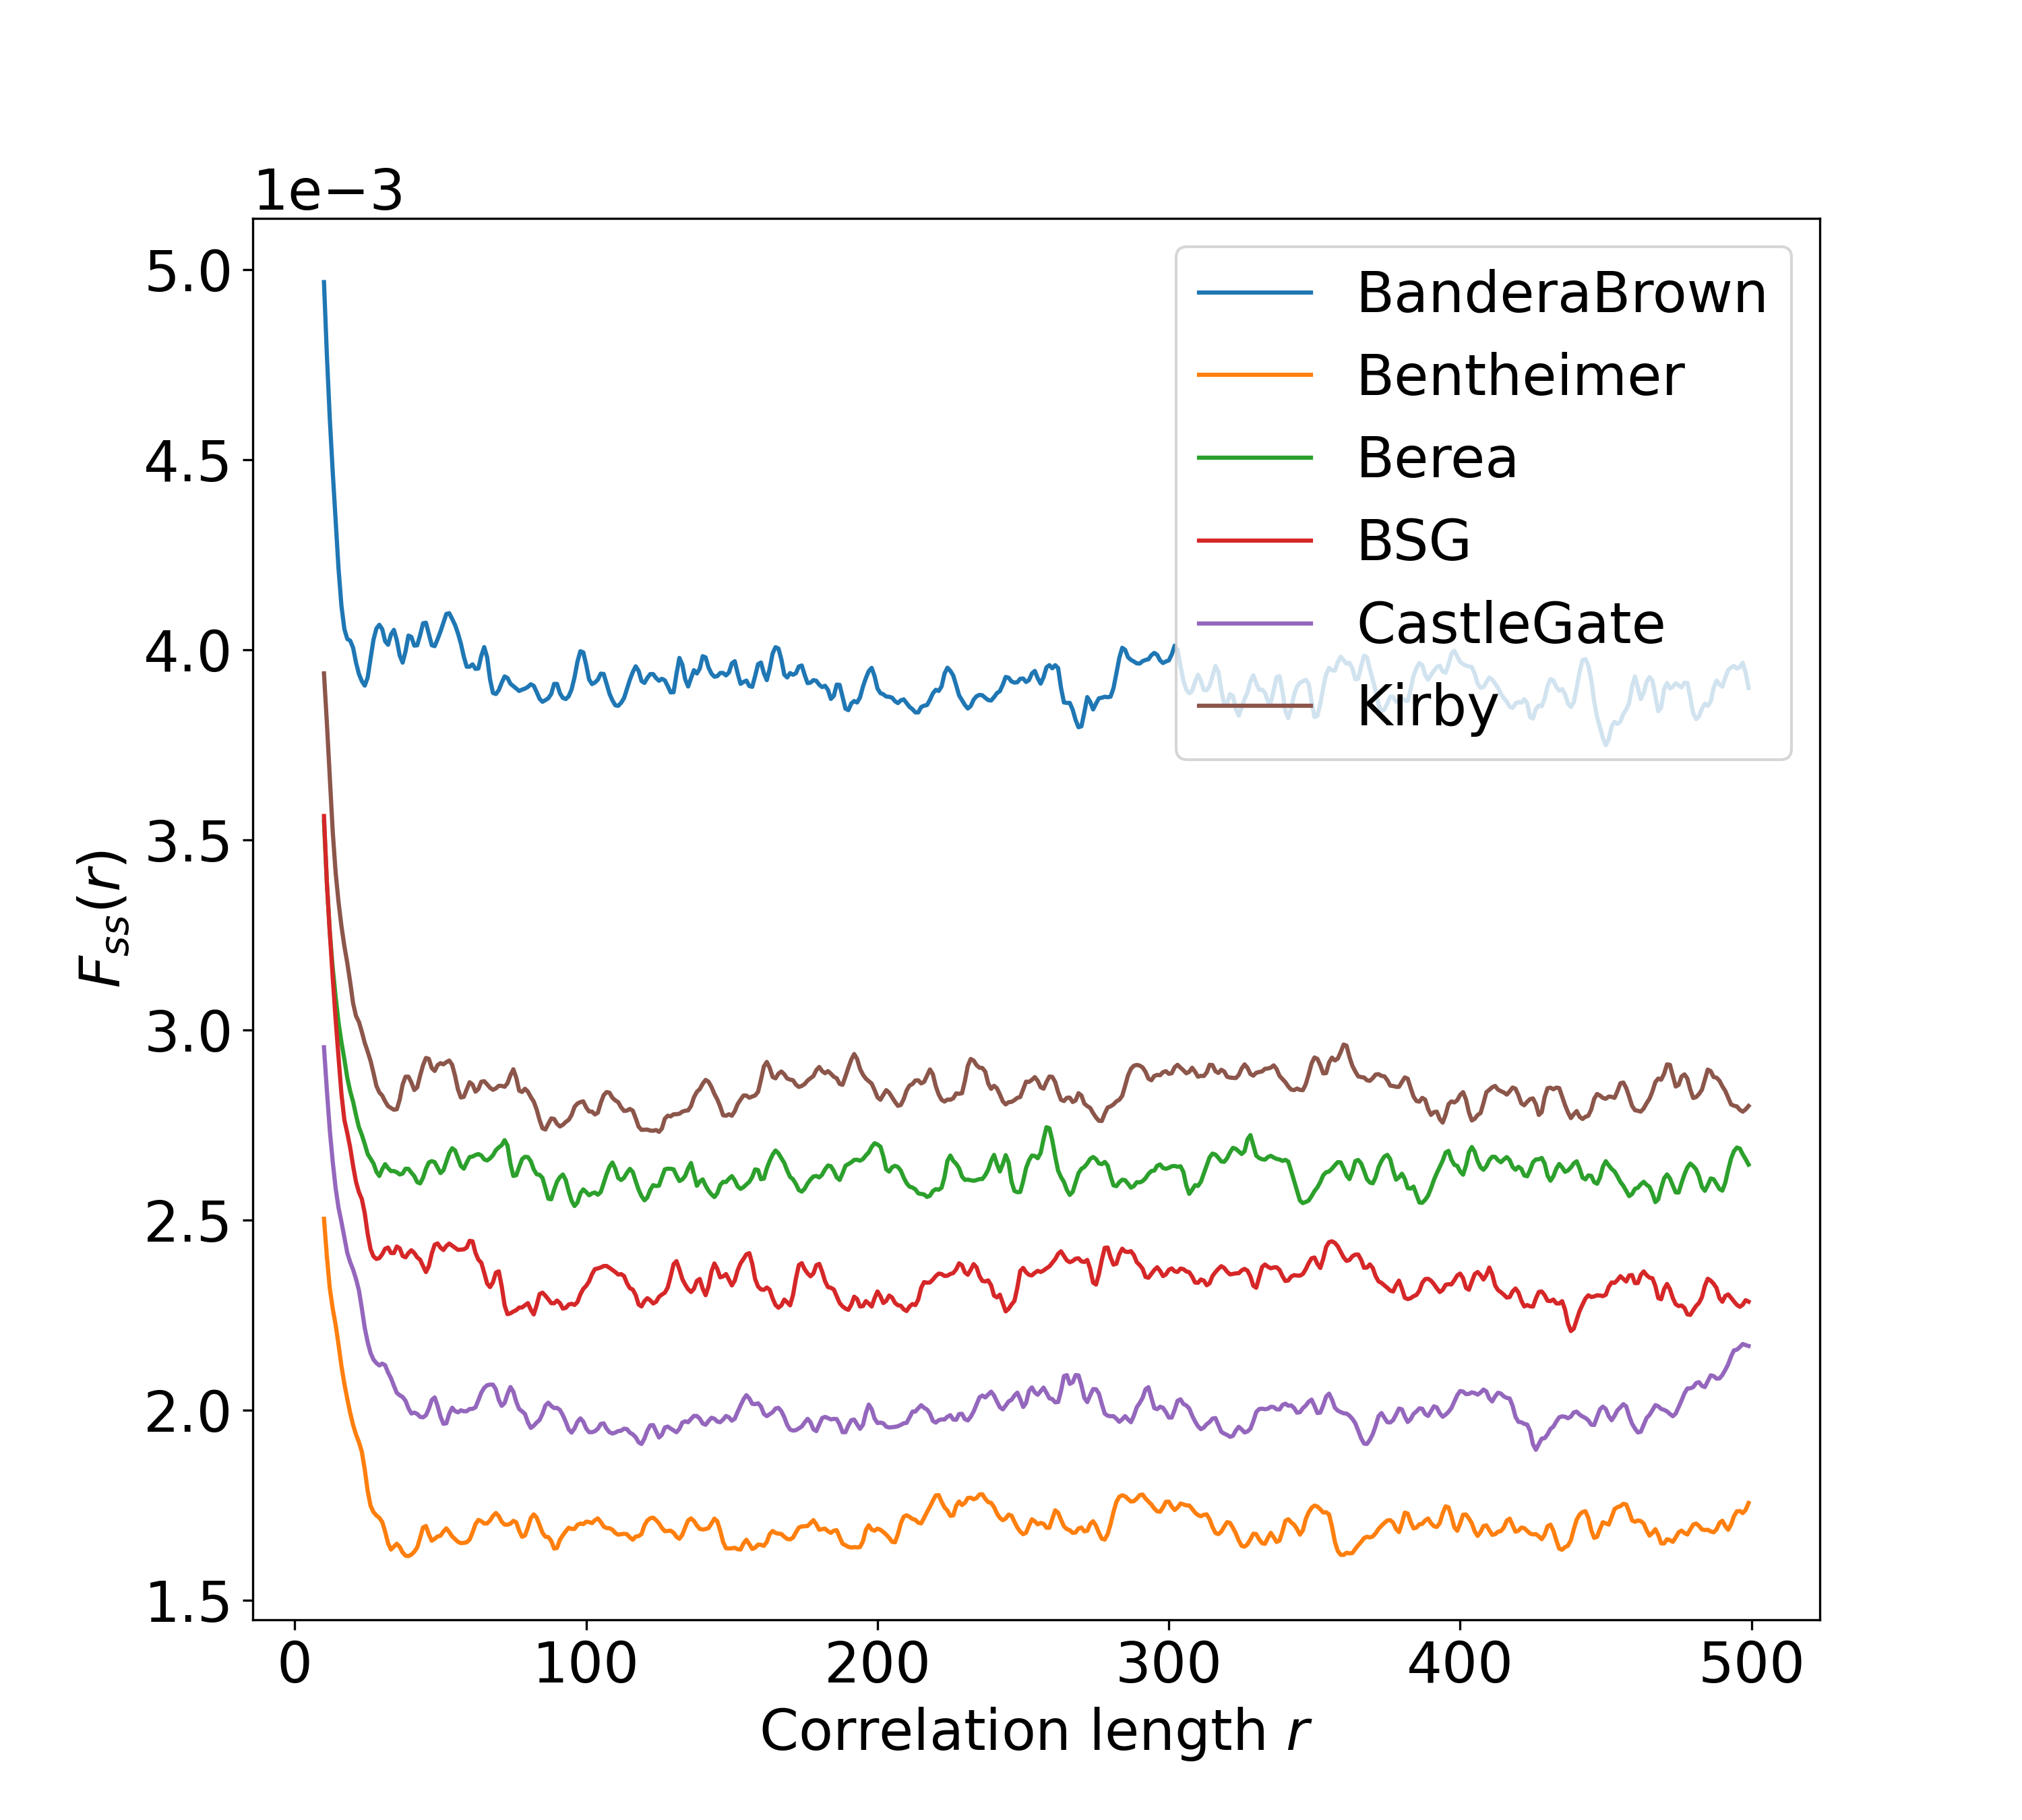
\includegraphics[width=0.3\linewidth]{real-data-plots/real-ss.png}
    \label{fig:real-ss}}
  \subfigure[$F_{sv}$ correlation function.]{
    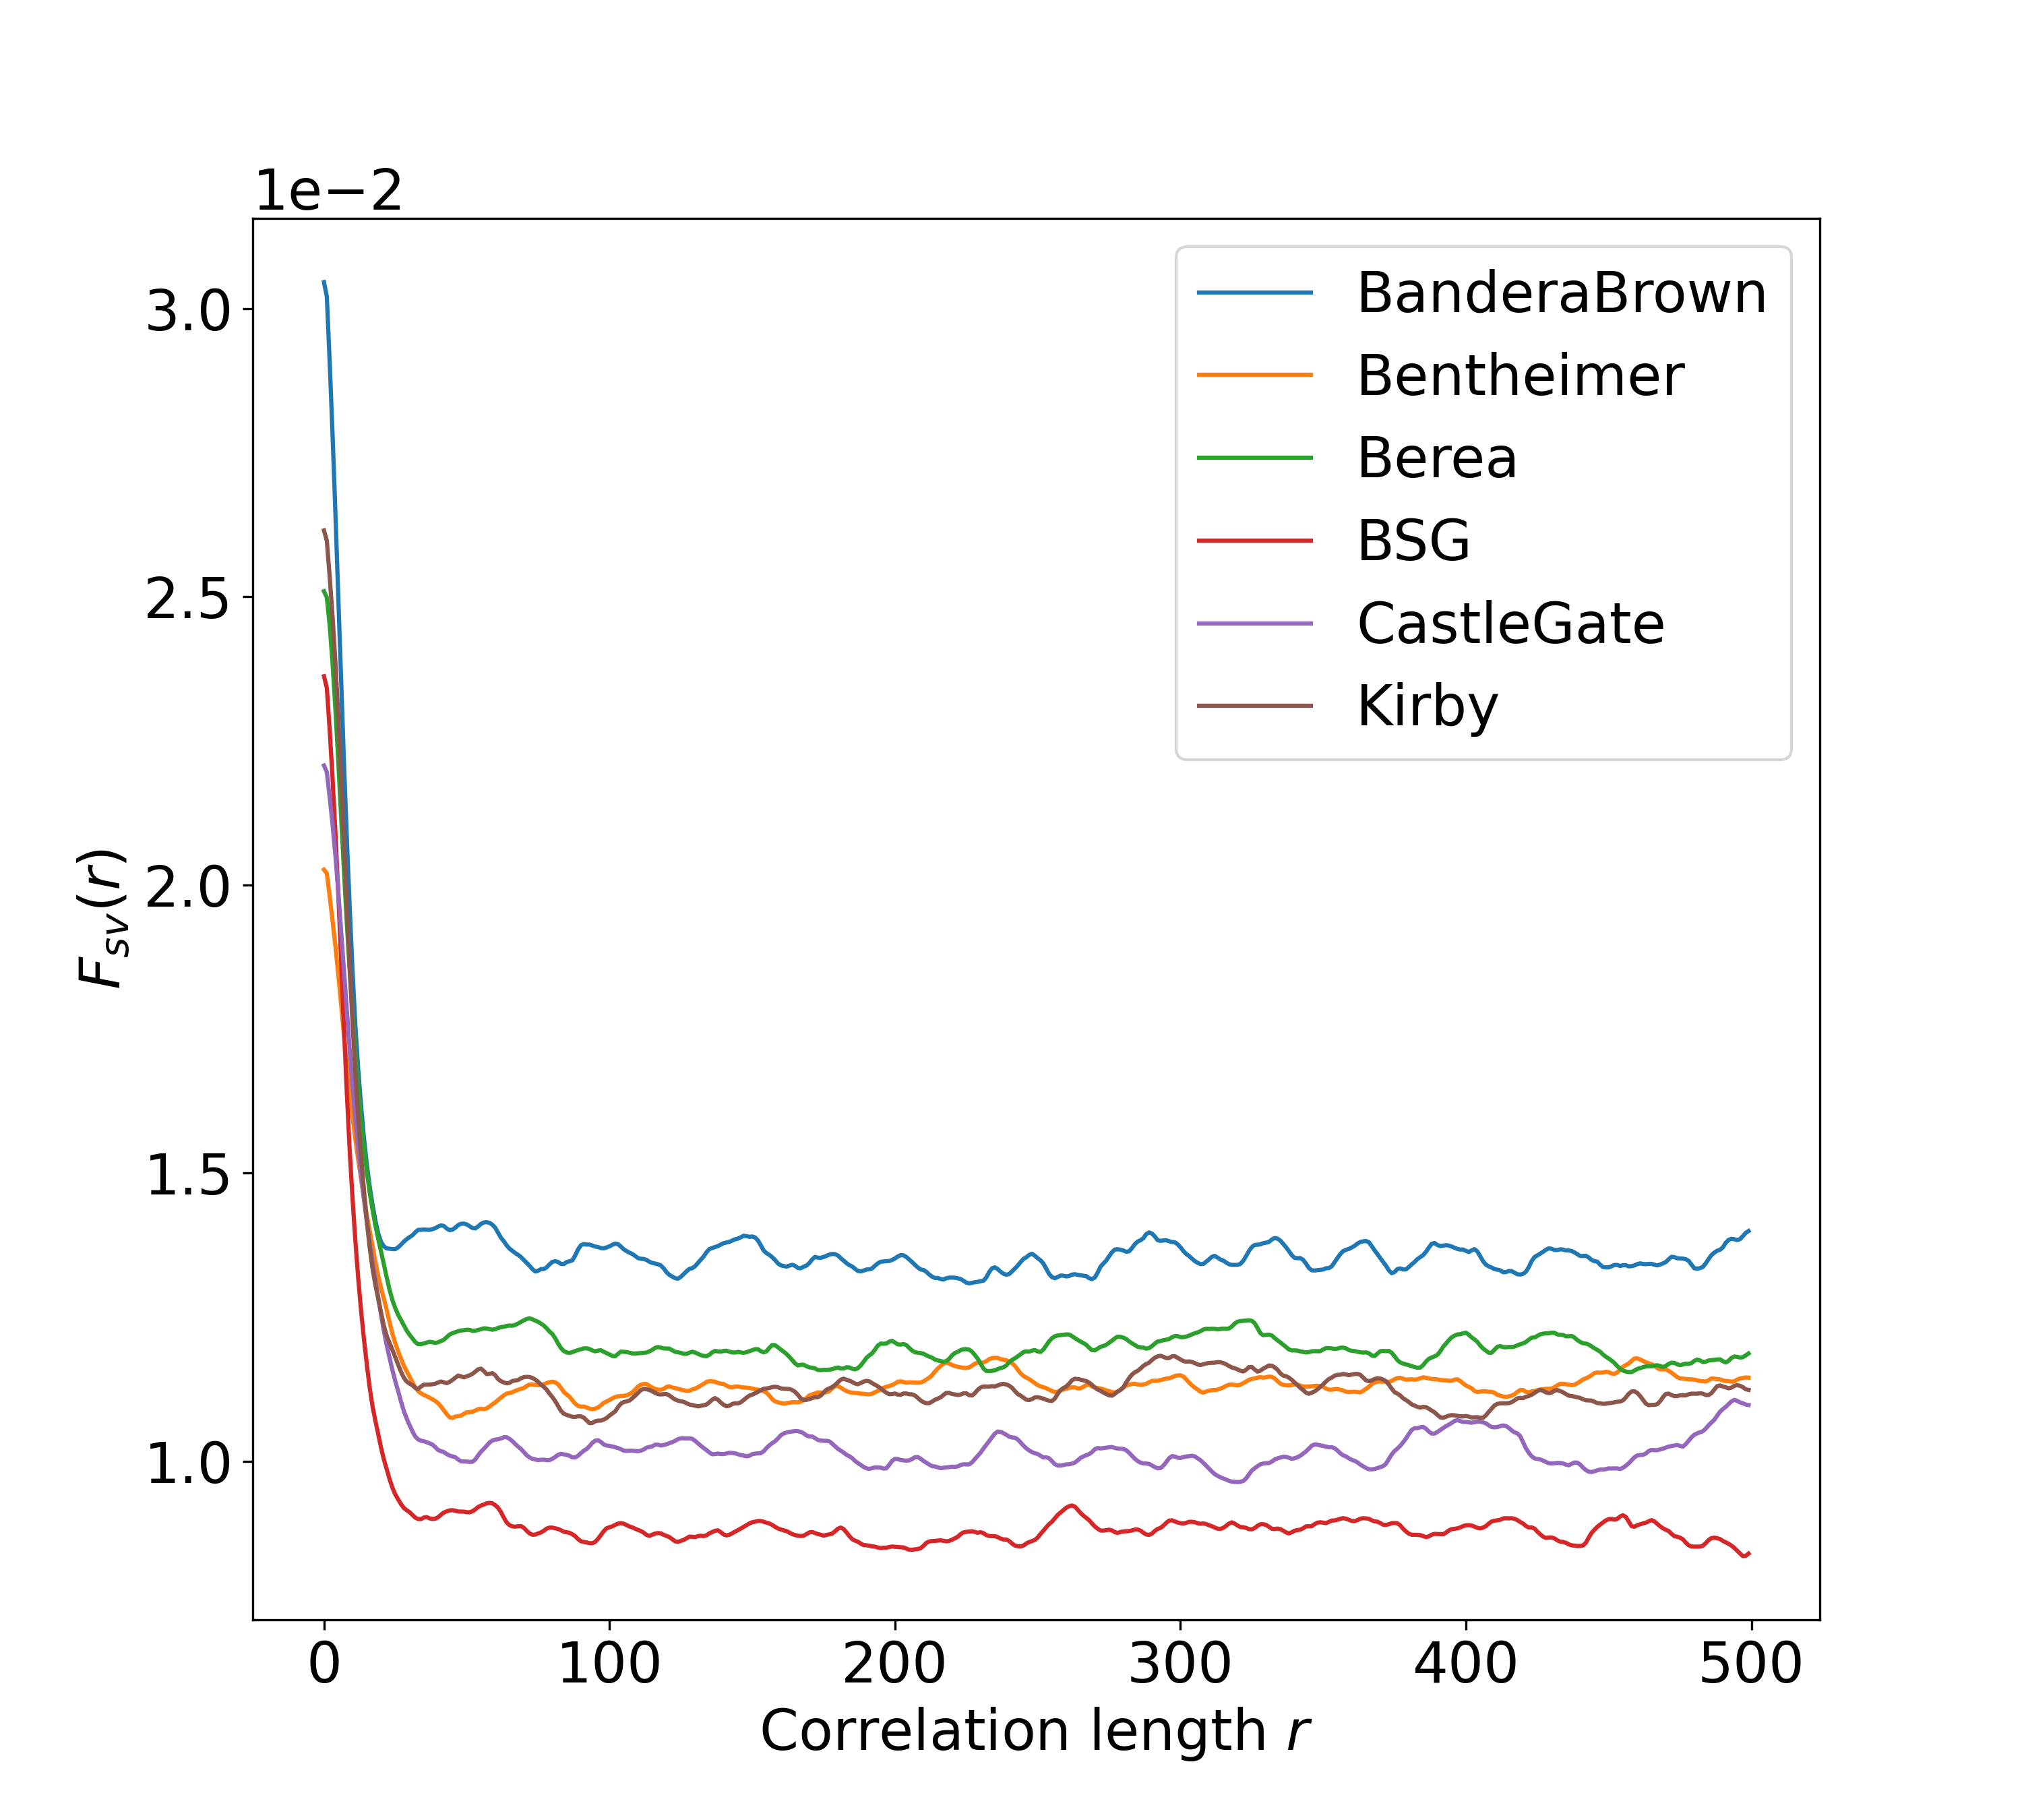
\includegraphics[width=0.3\linewidth]{real-data-plots/real-sv.png}
    \label{fig:real-sv}}
  \caption[]{Plots of correlation functions for images of sandstones.}
  \label{fig:real-data}
\end{figure*}

\section{Summary}
\label{sec:summary}
Text

\appendix
\section{Algorithm of computation of lineal-phase function}
\label{linpathalg}
The algorithm below calculates $L_2^{(phase)}$ correlation function for
one-dimensional array $a$. The result is an array of $L_2$ values for
correlation lengths from $0$ to $maxlen-1$. If $periodic$ is true (resp. false)
then periodic (resp. zero padding) boundary conditions are used. The entry point of the
algorithm is the function L2. The efficiency of the proposed algorithm is $O(n)$
where $n$ is the length of the array.

\begin{algorithmic}[1]
  \Procedure{countruns}{$a, len, phase$}
    \State $runslist \gets [\quad]$
    \State $runs \gets 0$
    \ForAll{$x \in a$}
      \If{$x = phase$}
        \State $runs \gets runs + 1$
      \ElsIf{$runs \ne 0$}
        \State $runslist \gets runs:runslist$
        \State $runs \gets 0$
      \EndIf
    \EndFor
    \If{$runs \ne 0$}
      \State $runslist \gets runs:runslist$
    \EndIf
    \State \textbf{return} $runslist$
  \EndProcedure
  \\
  \Procedure{updateruns}{$a, runs, n$}
    \For{$idx = 1,n$}
      \State $a[idx] \gets a[idx] + runs$
      \State $runs \gets runs - 1$
    \EndFor
  \EndProcedure
  \\
  \Procedure{updateperiodic}{$a, first, last, n$}
    \State $sum \gets first + last$
    \State $n \gets \min(n, sum)$
    \For{$idx = 1,n$}
      \State $a \gets \min(idx - 1, first, last, sum - (idx - 1))$
      \State $a[idx] \gets a[idx] + a$
    \EndFor
  \EndProcedure
  \\
  \Procedure{l2}{$a, phase, maxlen, periodic$}
    \State $success \gets zeros(maxlen)$
    \State $total \gets zeros(maxlen)$
    \State $len \gets length(a)$
    \State $nupdates \gets \min(len, maxlen)$
    \State $runs \gets countruns(a, maxlen, phase)$
    \ForAll{$run \in runs$}
      \State $updateruns(success, run, \min(run, maxlen))$
    \EndFor
    \If{$periodic$}
      \State $first \gets first(a)$
      \State $last \gets last(a)$
      \If{$first = last$}
        \State $updateperiodic(success, first, last, nupdates)$
      \EndIf
      \State Increment $total[\text{from} \, 1 \, \text{to} \, nupdates]$ by
      $len$
    \Else
      \State $updateruns(total, len, nupdates)$
    \EndIf
    \State \textbf{return} $success$ divided by $total$ element-wise.  
  \EndProcedure
\end{algorithmic}

\section{Algorithm for image rotation}
\label{rotating}

\begin{algorithmic}[1]
  \Procedure{rotate}{$a, direction, periodic$}
    \ForAll{$slice \in eachslice(a)$}
      \State $shift \gets get\_shift(slice, direction)$
      \State $rotated\_slice \gets circshift(slice, shift)$
      \If{$! periodic$}
        \State $rotated\_slice[end - shift:end] \gets -1$
      \EndIf
    \EndFor
  \State \textbf{return} $rotated$
  \EndProcedure
\end{algorithmic}

\bibliography{apssamp}
\end{document}
